\section{Results}
\label{sec:result}

A model of the observations in all data samples, described by a
likelihood function, is used to obtain a consistent prediction of the
SM backgrounds, and to test for the presence of new-physics signals if
the signal region is included in the maximum-likelihood fit. The
observation in each bin defined by the \njet, \nb, \scalht, and \HTmiss
variables is modelled as a Poisson-distributed variable around the SM
expectation and a potential signal contribution (assumed to be zero in
the following discussion), where the SM expectation is the sum over
the estimated contributions from all background processes according to
the methods described in Section~\ref{}. 

The non-multijet backgrounds, which comprise the \wlj and \ttj (``lost
lepton'') backgrounds, the residual contributions from other
processes, such as single top, diboson, and Drell-Yan production, and
the irreducible \znunuj background, are related to the expected yields
in the \mj, \mmj, and \gj control samples via the transfer factors
derived from simulation, as described in
Section~\ref{needreftocontrolregions}. For event categories that
satisfy $\nb < 2$, all three of the aforementioned control samples are
considered in the estimation of the \znunuj background. For events
with $\nb > 1$, only the \mj control sample is used to determine the
total contribution from all non-multijet backgrounds in the signal
region. 
Estimates of the contribution from multijet events in the control and
signal regions are determined, respectively, directly from simulation
or according to the method described in Section~\ref{sec:qcd}, and are
included in the likelihood function.

%The likelihood function is the product of Poisson probability density
%functions, one for each signal region, and constraint terms that
%account for uncertainties in the background predictions and signal
%yields. These uncertainties are treated as nuisance parameters with
%log-normal probability density functions. Correlations are taken into
%account where appropriate.

The systematic uncertainties summarised in Table~\ref{tab:bkgd_systs}
are accommodated in the likelihood function through the use of
nuisance parameters, the measurements of which are assumed to follow a
log-normal distribution, and alternative templates that describe the
uncertainties in the \HTmiss distributions. A vertical template morphing
scheme~\cite{Prosper:1306523} is used to interpolate between the
nominal and alternative \HTmiss templates. A nuisance parameter controls
the interpolation, which is gaussian distributed with a mean of zero
and a standard deviation of one, where $\pm$1 corresponds to the
alternative templates for a $\pm$1$\sigma$ variation in the
uncertainty. Each template is interpolated quadratically between
$\pm$1$\sigma$, and a linear extrapolation is employed beyond these
bounds.

%Figure 7 presents one-dimensional projections of the results in HTmiss
%or HT after criteria are  imposed, as indicated in the legends, 
%In each case, example distributions are shown for two signal scenarios
%not excluded by our Run 1 studies [22, 23], explained below.

The ``pre-fit'' result of this search, which considers the
observations in the control regions only, is summarised in
Tables~\ref{tab:mono}, \ref{tab:asym}, and \ref{tab:sym} for,
respectively, the monojet, asymmetric, and symmetric topologies. This
result is based on an estimate of the \znunuj background using
observations in multiple control regions as described by the
likelihood function, maximised over all fit
parameters. Tables~\ref{tab:mono}, \ref{tab:asym}, and \ref{tab:sym}
also summarise the ``post-fit'' result, which is based on a
maximum-likelihood fit to observations in the signal region as well as
the control regions. No significant tension is observed between the
data and SM expectations in the signal region (and control regions),
and the data are well described by the background-only hypothesis. A
saturated likelihood model~\cite{} is used as a goodness-of-fit test
to determine the compatibility of the observed yields with the
expectations from only SM processes (\ie the background-only
hypothesis). A $p$-value of 0.XX\% is observed for the fit over the
full signal region, and $p$-values in the range 0.04--1.00\% and
consistent with a uniform distribution when considering events
categorised according to \njet. 
% Njet-binned p-values taken from http://www.hep.ph.ic.ac.uk/~mc3909/Log/16-04/16-04-27/pValues/pValuesnB.pdf

%\begin{figure*}[tb]
%  \begin{center}
%    \subfigure[\texttt{T1qqqq}]{
%      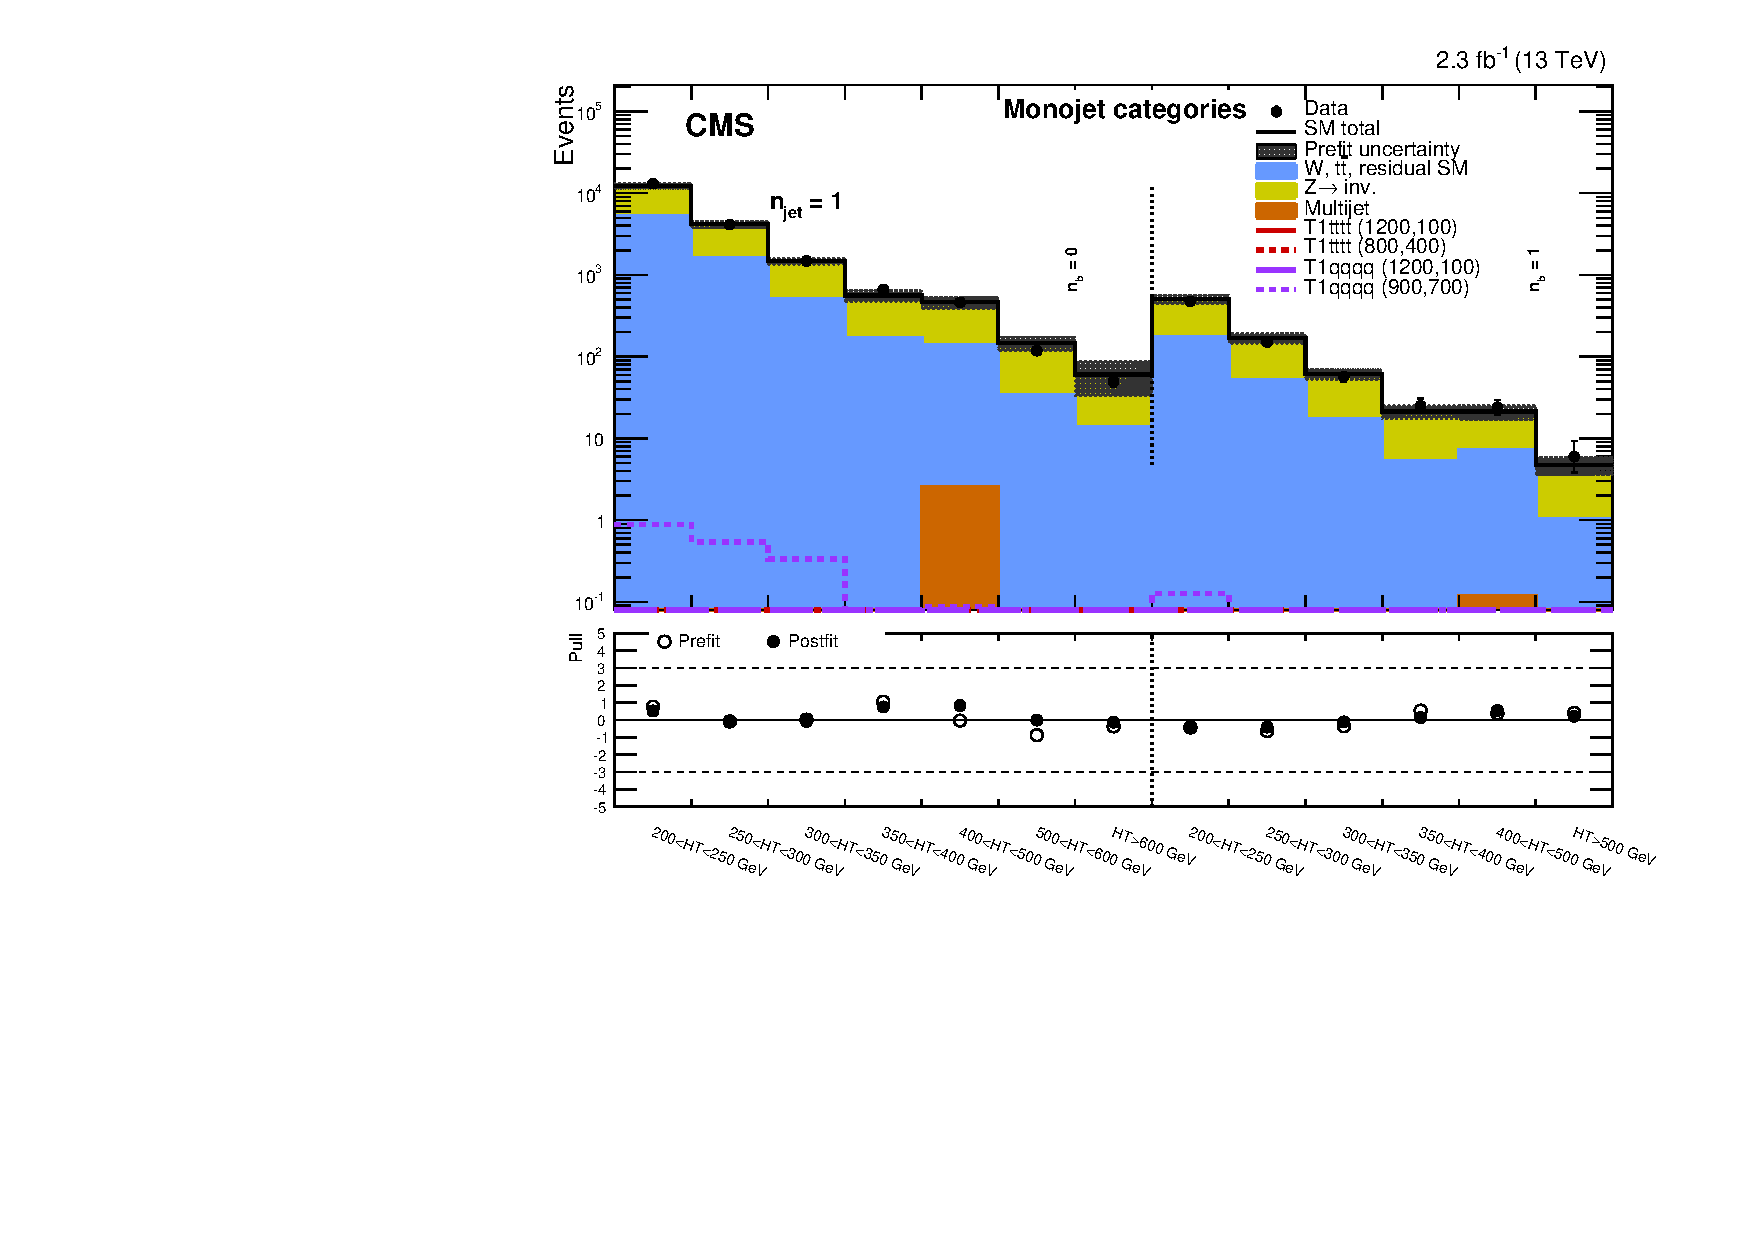
\includegraphics[width=0.50\textwidth]{figures/result/summaryPlot_Monojet_prefit_overlay_fit_b}
%      \label{fig:result_mono}
%    } \\
%    \subfigure[\texttt{T2qq}]{
%      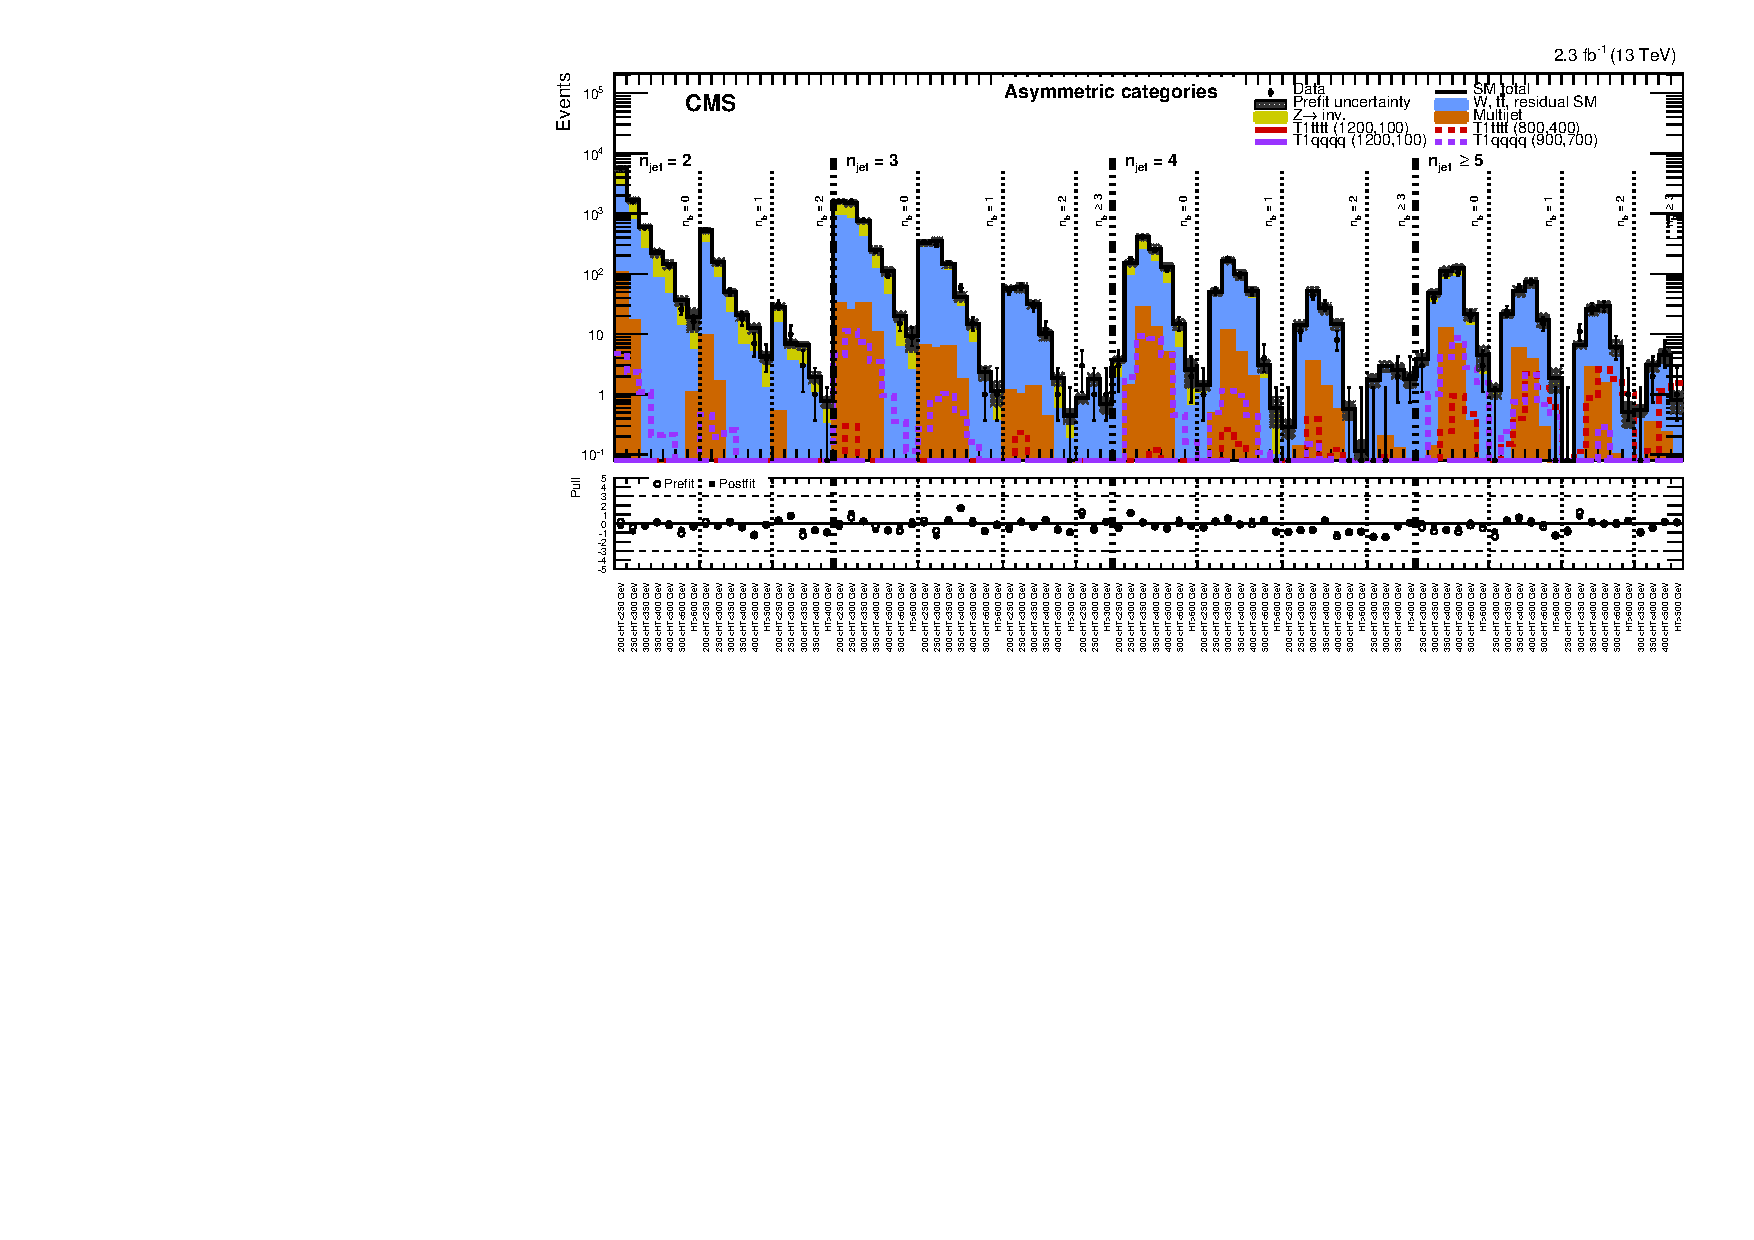
\includegraphics[width=0.90\textwidth]{figures/result/summaryPlot_Asymmetric_prefit_overlay_fit_b}
%      \label{fig:result_asym}
%    } \\
%    \subfigure[\texttt{T1bbbb}]{
%      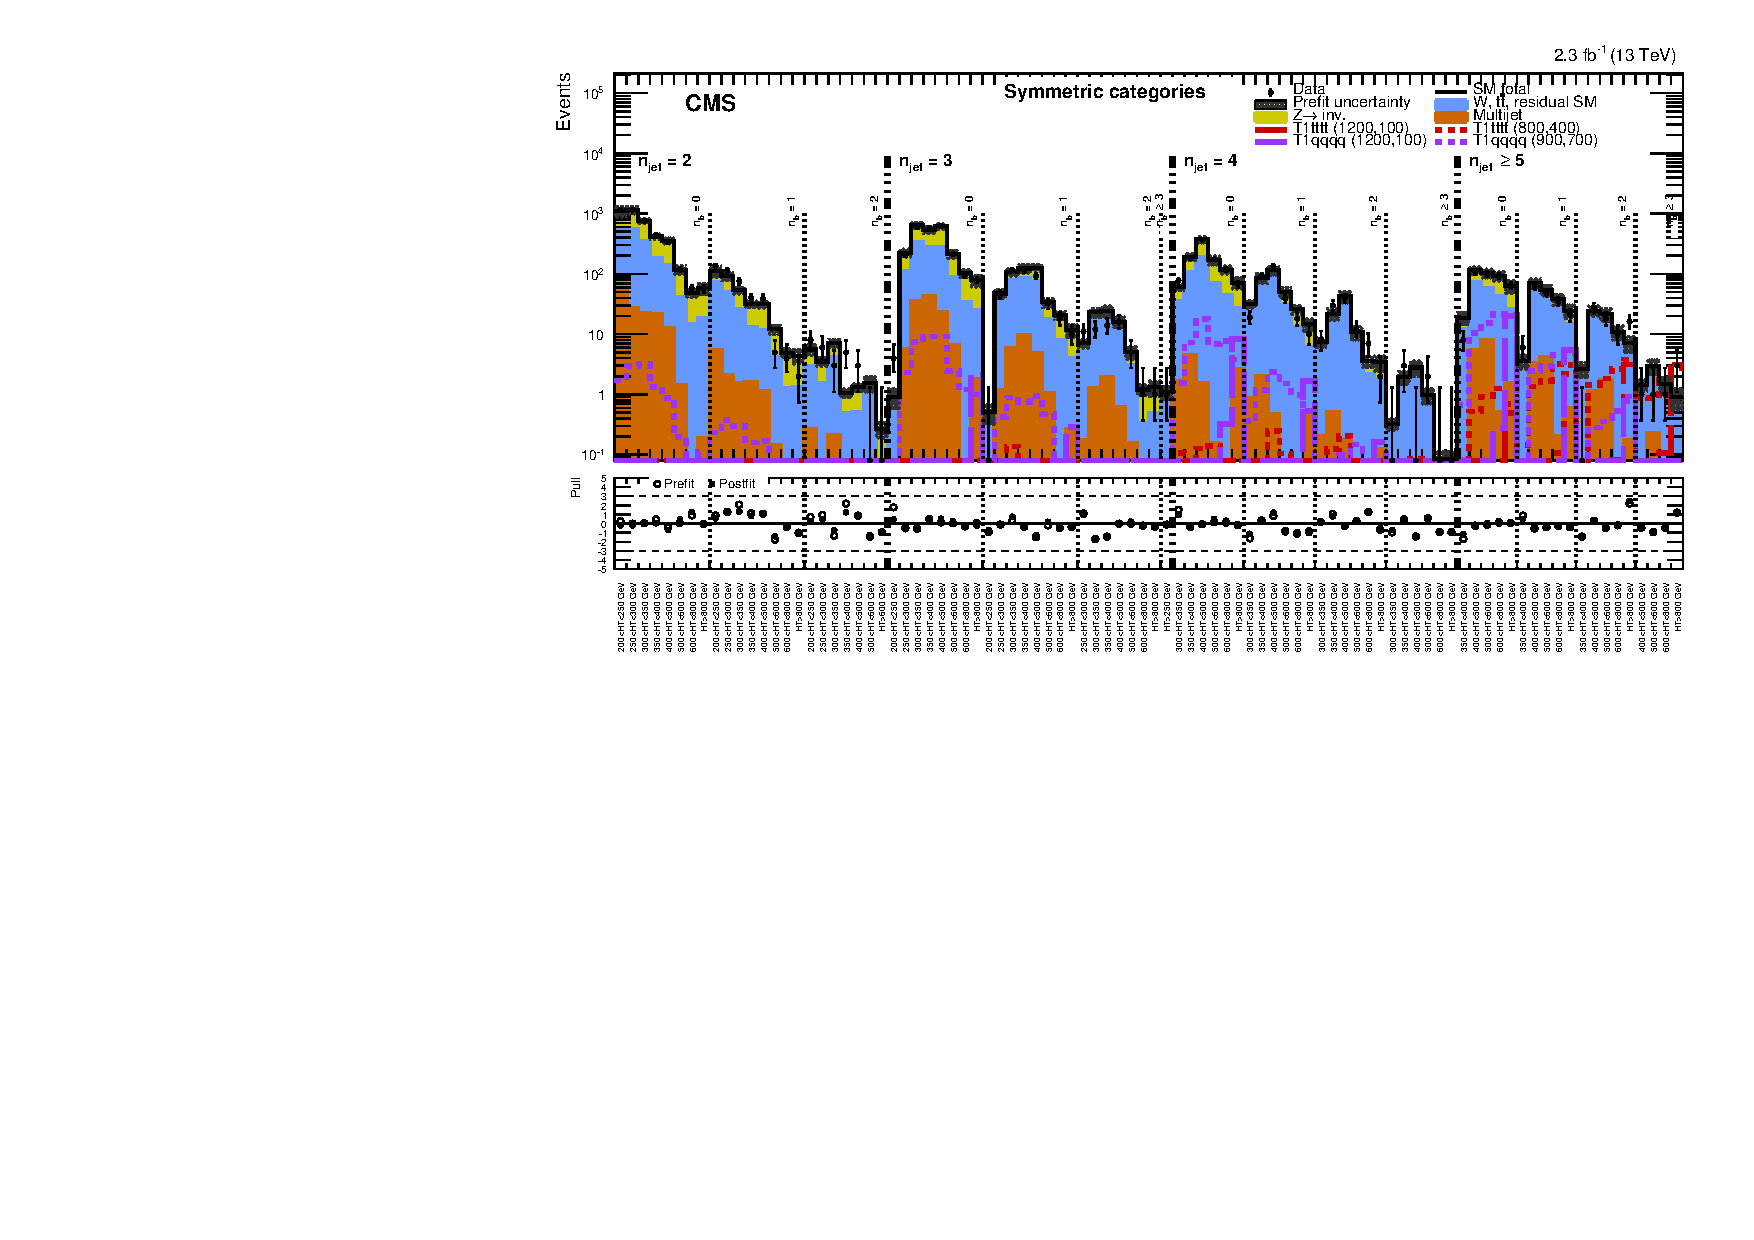
\includegraphics[width=0.90\textwidth]{figures/result/summaryPlot_Symmetric_prefit_overlay_fit_b}
%      \label{fig:result_symm}
%    } 
%    \caption{Caption here. 
%    }
%    \label{fig:result}
%  \end{center}
%\end{figure*}

\begin{figure}[!h]
  \begin{center}
    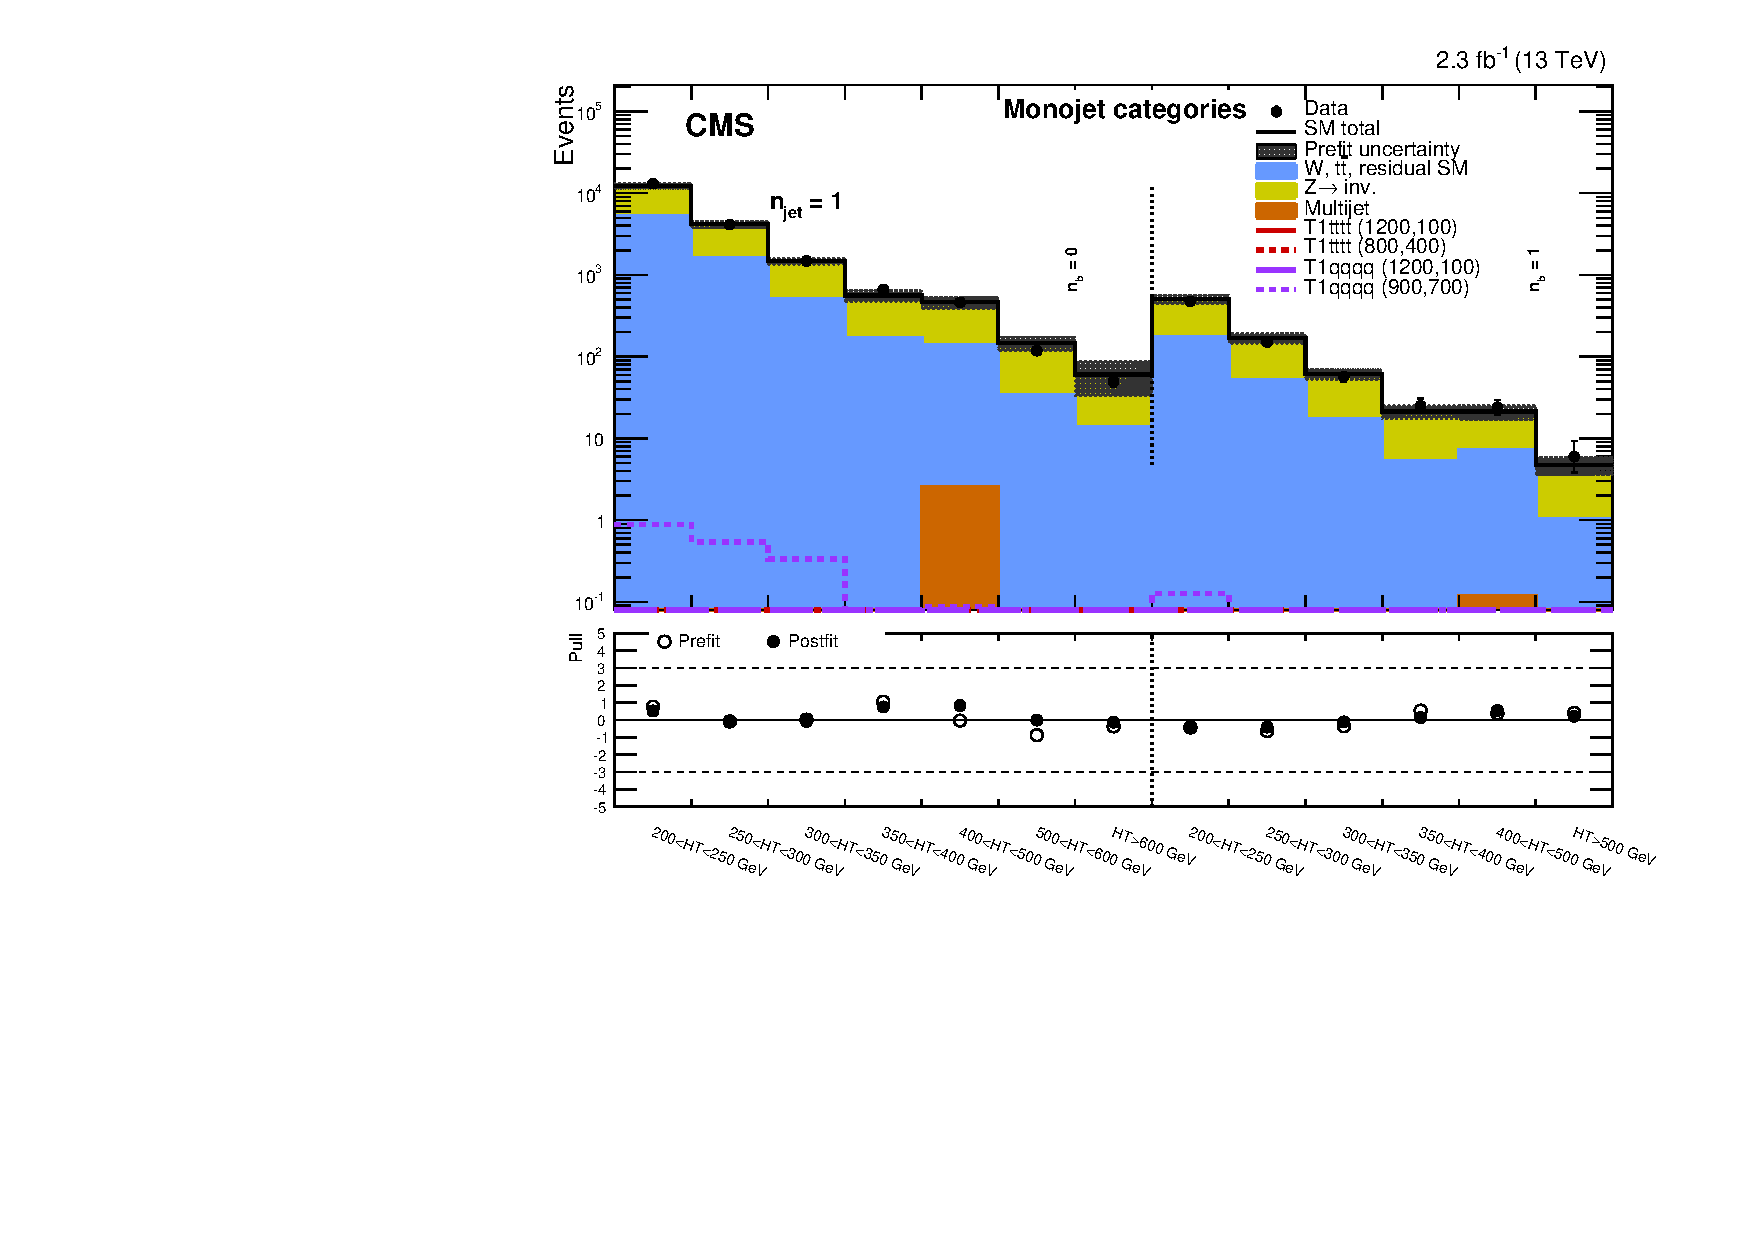
\includegraphics[width=0.49\textwidth]{figures/result/summaryPlot_Monojet_prefit_overlay_fit_b}
    \caption{Caption here.}
    \label{fig:result}
  \end{center}
\end{figure}

\begin{figure*}[!h]
  \begin{center}
    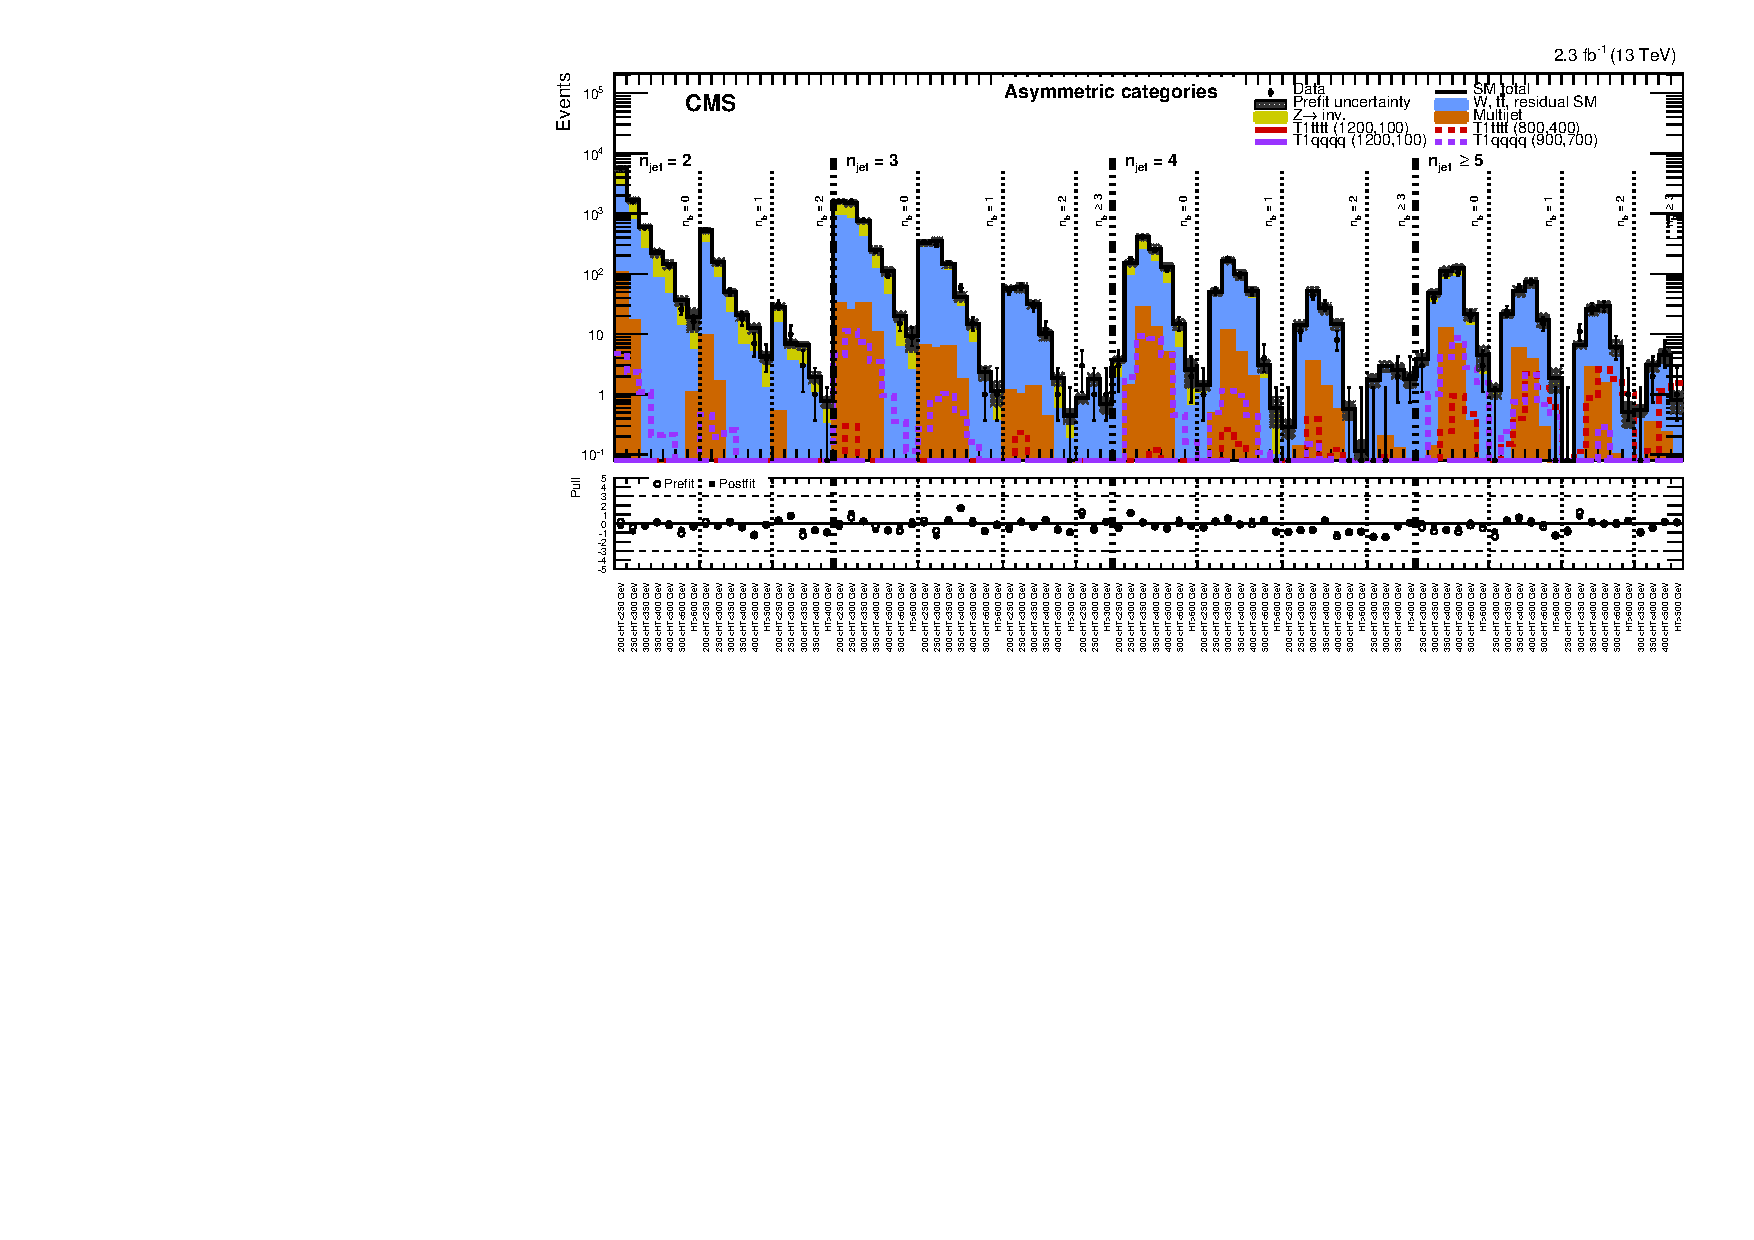
\includegraphics[angle=90,width=0.60\textwidth]{figures/result/summaryPlot_Asymmetric_prefit_overlay_fit_b}
    \caption{Caption here.}
    \label{fig:result}
  \end{center}
\end{figure*}

\begin{figure*}[!h]
  \begin{center}
    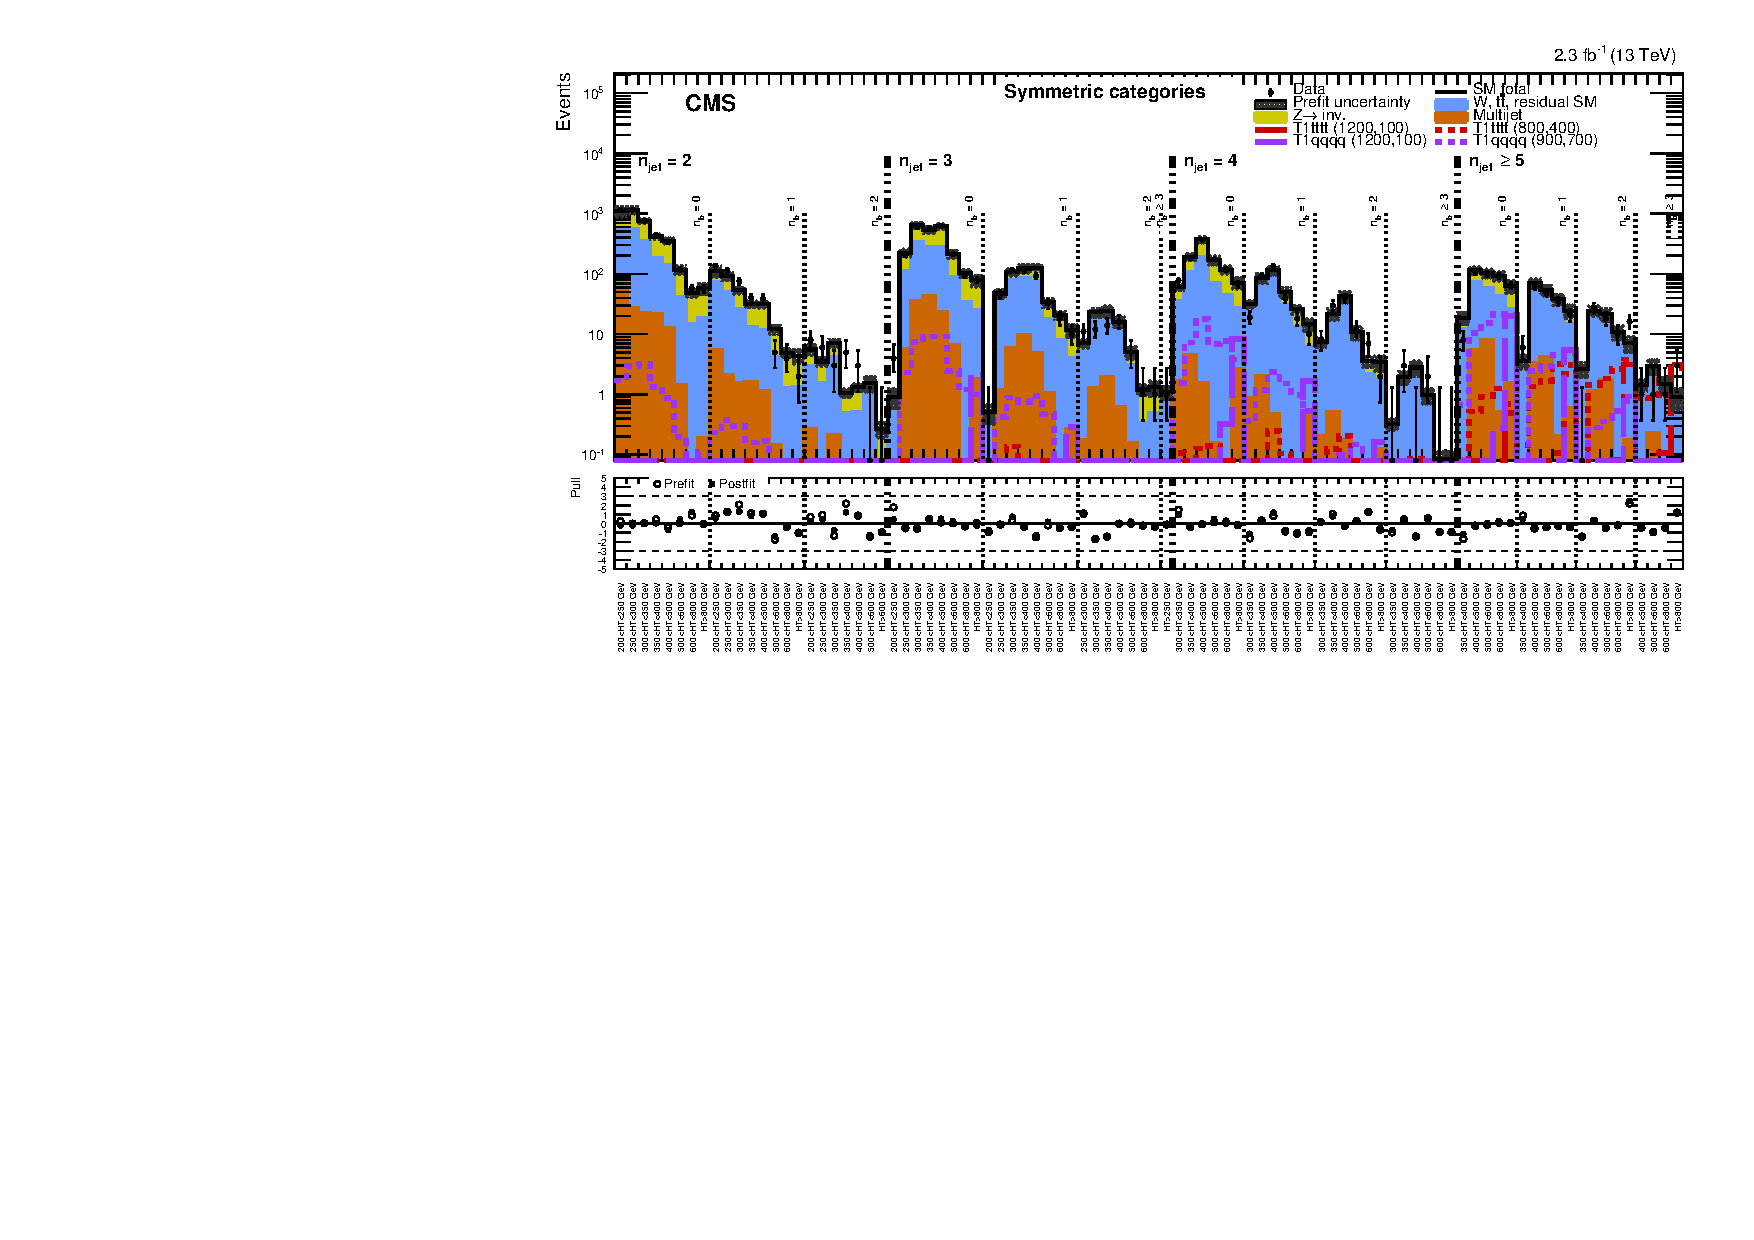
\includegraphics[angle=90,width=0.60\textwidth]{figures/result/summaryPlot_Symmetric_prefit_overlay_fit_b}
    \caption{Caption here.}
    \label{fig:result}
  \end{center}
\end{figure*}

%\begin{table}[h!]
\scriptsize
\centering
\caption{
  Observed data counts, ``pre-fit'' and ``post-fit'' background expectations  
  for all the \scalht bins and \njet, \nb multiplicity in the monojet event category. 
  The uncertainties include statistical as well as systematic contributions. 
  \label{tab:predewkdata_sig_comb_mono}}  
\scalebox{0.85}{\begin{tabular}{lccccccccc}
	\hline\hline
                    &              & \multicolumn{8}{c}{\scalht (\gev)}                                                                                                                                    \\ 
                    & (\njet, \nb) & 200-250               & 250-300              & 300-350              & 350-400            & 400-500            & 500-600            & 600-800           & 800-$\infty$ \\ [0.8ex] 
\hline
 Data & $(1j,0)$ & $13094$ & $4130$ & $1477$ & $663$ & $461$ & $118$ & $50$ & -- \\[0.5ex]
 SM pre-fit & $(1j,0)$ & $12319.3\pm985.8$ & $4167.9\pm384.1$ & $1474.1\pm155.2$ & $559.8\pm95.2$ & $463.1\pm74.5$ & $145.6\pm29.1$ & $60.4\pm25.1$ & -- \\[0.5ex]
 SM post-fit & $(1j,0)$ & $13012.3\pm112.8$ & $4133.5\pm57.7$ & $1480.8\pm33.9$ & $638.0\pm21.4$ & $439.5\pm16.0$ & $118.1\pm7.0$ & $51.3\pm6.4$ & -- \\[0.5ex]
 Data & $(1j,1)$ & $475$ & $151$ & $57$ & $25$ & $24$ & $6$ & -- & -- \\[0.5ex]
 SM pre-fit & $(1j,1)$ & $505.3\pm64.3$ & $169.6\pm24.6$ & $61.3\pm10.3$ & $21.3\pm4.5$ & $21.0\pm4.4$ & $4.7\pm1.3$ & -- & -- \\[0.5ex]
 SM post-fit & $(1j,1)$ & $488.4\pm18.1$ & $157.9\pm11.0$ & $58.1\pm6.2$ & $24.1\pm3.8$ & $20.8\pm2.6$ & $5.3\pm1.4$ & -- & -- \\[0.5ex]

	\hline
	\hline
\end{tabular}}
\end{table}

%\begin{table}[h!]
\scriptsize
\centering
\caption{
  Observed data counts, ``pre-fit'' and ``post-fit'' background expectations  
  for all the \scalht bins and \njet, \nb multiplicity in the asymmetric event category. 
  The uncertainties include statistical as well as systematic contributions. 
  \label{tab:predewkdata_sig_comb_asym}}  
\scalebox{0.85}{\begin{tabular}{lccccccccc}
	\hline\hline
                    &                   & \multicolumn{8}{c}{\scalht (\gev)}                                                                                                                              \\ 
                    & (\njet, \nb)      & 200-250              & 250-300              & 300-350            & 350-400            & 400-500            & 500-600          & 600-800          & 800-$\infty$ \\ [0.8ex] 
\hline

 Data & $(2a,0)$ & $5788$ & $1585$ & $584$ & $232$ & $139$ & $26$ & $16$ & -- \\[0.5ex]
 SM pre-fit & $(2a,0)$ & $5890.6\pm544.0$ & $1695.0\pm180.5$ & $601.3\pm65.1$ & $224.3\pm38.4$ & $144.4\pm25.0$ & $36.4\pm7.1$ & $21.0\pm8.1$ & -- \\[0.5ex]
 SM post-fit & $(2a,0)$ & $5831.5\pm81.6$ & $1621.6\pm35.0$ & $581.0\pm17.9$ & $227.5\pm9.5$ & $136.5\pm6.4$ & $30.0\pm2.6$ & $18.3\pm3.2$ & -- \\[0.5ex]
 Data & $(2a,1)$ & $536$ & $152$ & $51$ & $18$ & $7$ & $4$ & -- & -- \\[0.5ex]
 SM pre-fit & $(2a,1)$ & $543.8\pm62.0$ & $161.7\pm22.6$ & $49.3\pm7.7$ & $20.5\pm3.9$ & $12.9\pm2.6$ & $4.3\pm1.0$ & -- & -- \\[0.5ex]
 SM post-fit & $(2a,1)$ & $541.0\pm16.4$ & $153.8\pm7.1$ & $49.7\pm3.7$ & $19.7\pm2.2$ & $10.7\pm1.4$ & $4.0\pm1.0$ & -- & -- \\[0.5ex]
 Data & $(2a,2)$ & $31$ & $10$ & $3$ & $1$ & $0$ & -- & -- & -- \\[0.5ex]
 SM pre-fit & $(2a,2)$ & $29.7\pm4.0$ & $7.2\pm1.2$ & $6.5\pm1.2$ & $2.0\pm0.5$ & $0.8\pm0.2$ & -- & -- & -- \\[0.5ex]
 SM post-fit & $(2a,2)$ & $29.5\pm3.5$ & $7.4\pm1.2$ & $5.0\pm1.1$ & $1.8\pm0.6$ & $0.6\pm0.3$ & -- & -- & -- \\[0.5ex]
 Data & $(3a,0)$ & $1599$ & $1609$ & $777$ & $239$ & $95$ & $15$ & $9$ & -- \\[0.5ex]
 SM pre-fit & $(3a,0)$ & $1669.4\pm163.3$ & $1529.4\pm171.2$ & $822.9\pm127.9$ & $272.3\pm60.5$ & $111.3\pm18.2$ & $19.7\pm4.0$ & $9.3\pm4.1$ & -- \\[0.5ex]
 SM post-fit & $(3a,0)$ & $1624.8\pm39.6$ & $1561.5\pm44.5$ & $781.7\pm28.8$ & $258.7\pm13.4$ & $100.9\pm5.4$ & $16.5\pm1.7$ & $8.0\pm1.5$ & -- \\[0.5ex]
 Data & $(3a,1)$ & $340$ & $299$ & $152$ & $59$ & $15$ & $1$ & $1$ & -- \\[0.5ex]
 SM pre-fit & $(3a,1)$ & $340.3\pm38.6$ & $357.2\pm51.6$ & $156.6\pm28.2$ & $46.1\pm12.0$ & $14.6\pm2.7$ & $2.3\pm0.7$ & $1.1\pm0.5$ & -- \\[0.5ex]
 SM post-fit & $(3a,1)$ & $340.7\pm12.6$ & $335.8\pm13.1$ & $148.6\pm7.9$ & $47.1\pm3.6$ & $13.0\pm1.4$ & $2.0\pm0.5$ & $1.0\pm0.4$ & -- \\[0.5ex]
 Data & $(3a,2)$ & $52$ & $62$ & $29$ & $12$ & $1$ & $0$ & -- & -- \\[0.5ex]
 SM pre-fit & $(3a,2)$ & $59.3\pm7.6$ & $61.9\pm10.1$ & $34.2\pm7.0$ & $11.2\pm3.2$ & $1.9\pm0.4$ & $0.4\pm0.1$ & -- & -- \\[0.5ex]
 SM post-fit & $(3a,2)$ & $58.3\pm4.6$ & $60.1\pm3.8$ & $31.3\pm2.7$ & $11.1\pm1.5$ & $1.5\pm0.4$ & $0.4\pm0.2$ & -- & -- \\[0.5ex]
 Data & $(3a,\geq 3)$ & $3$ & $1$ & $1$ & -- & -- & -- & -- & -- \\[0.5ex]
 SM pre-fit & $(3a,\geq 3)$ & $0.9\pm0.2$ & $1.9\pm0.4$ & $0.8\pm0.2$ & -- & -- & -- & -- & -- \\[0.5ex]
 SM post-fit & $(3a,\geq 3)$ & $1.3\pm0.5$ & $1.5\pm0.6$ & $0.8\pm0.4$ & -- & -- & -- & -- & -- \\[0.5ex]
 Data & $(4a,0)$ & $3$ & $178$ & $412$ & $246$ & $119$ & $15$ & $2$ & -- \\[0.5ex]
 SM pre-fit & $(4a,0)$ & $3.8\pm0.5$ & $153.4\pm18.5$ & $462.8\pm89.5$ & $285.1\pm64.1$ & $142.4\pm22.6$ & $14.7\pm3.2$ & $2.6\pm1.2$ & -- \\[0.5ex]
 SM post-fit & $(4a,0)$ & $4.1\pm1.0$ & $159.3\pm10.8$ & $418.0\pm19.5$ & $256.7\pm14.2$ & $128.0\pm7.6$ & $12.9\pm1.7$ & $2.2\pm0.6$ & -- \\[0.5ex]
 Data & $(4a,1)$ & $1$ & $53$ & $180$ & $96$ & $51$ & $4$ & $0$ & -- \\[0.5ex]
 SM pre-fit & $(4a,1)$ & $1.4\pm0.3$ & $51.5\pm7.5$ & $189.7\pm39.6$ & $108.1\pm25.9$ & $55.6\pm10.1$ & $3.1\pm0.8$ & $0.6\pm0.3$ & -- \\[0.5ex]
 SM post-fit & $(4a,1)$ & $1.6\pm0.5$ & $50.7\pm4.6$ & $172.6\pm9.2$ & $98.9\pm6.8$ & $49.0\pm3.9$ & $2.9\pm0.6$ & $0.5\pm0.1$ & -- \\[0.5ex]
 Data & $(4a,2)$ & $0$ & $11$ & $44$ & $30$ & $8$ & $0$ & $0$ & -- \\[0.5ex]
 SM pre-fit & $(4a,2)$ & $0.3\pm0.1$ & $14.6\pm2.4$ & $58.5\pm12.8$ & $30.0\pm7.8$ & $15.6\pm3.3$ & $0.6\pm0.2$ & $0.1\pm0.1$ & -- \\[0.5ex]
 SM post-fit & $(4a,2)$ & $0.3\pm0.2$ & $13.9\pm1.5$ & $51.6\pm4.3$ & $28.7\pm2.9$ & $12.7\pm1.6$ & $0.6\pm0.2$ & $0.1\pm0.0$ & -- \\[0.5ex]
 Data & $(4a,\geq 3)$ & -- & $0$ & $0$ & $2$ & $2$ & -- & -- & -- \\[0.5ex]
 SM pre-fit & $(4a,\geq 3)$ & -- & $1.8\pm0.4$ & $3.2\pm0.8$ & $2.8\pm0.8$ & $1.9\pm0.5$ & -- & -- & -- \\[0.5ex]
 SM post-fit & $(4a,\geq 3)$ & -- & $1.3\pm0.5$ & $2.4\pm0.8$ & $2.3\pm0.7$ & $2.1\pm0.6$ & -- & -- & -- \\[0.5ex]
 Data & $(\geq 5a,0)$ & -- & $3$ & $40$ & $96$ & $105$ & $20$ & $3$ & -- \\[0.5ex]
 SM pre-fit & $(\geq 5a,0)$ & -- & $3.9\pm1.1$ & $49.2\pm8.4$ & $137.6\pm40.4$ & $138.2\pm25.5$ & $22.0\pm5.1$ & $4.5\pm2.0$ & -- \\[0.5ex]
 SM post-fit & $(\geq 5a,0)$ & -- & $2.9\pm1.3$ & $43.5\pm4.7$ & $107.8\pm8.9$ & $114.4\pm8.6$ & $19.6\pm2.6$ & $3.3\pm0.9$ & -- \\[0.5ex]
 Data & $(\geq 5a,1)$ & -- & $0$ & $24$ & $60$ & $74$ & $15$ & $0$ & -- \\[0.5ex]
 SM pre-fit & $(\geq 5a,1)$ & -- & $1.2\pm0.4$ & $22.0\pm3.9$ & $64.5\pm20.4$ & $80.0\pm16.7$ & $17.9\pm4.8$ & $1.9\pm0.9$ & -- \\[0.5ex]
 SM post-fit & $(\geq 5a,1)$ & -- & $0.8\pm0.5$ & $22.2\pm3.0$ & $57.4\pm5.9$ & $71.9\pm5.7$ & $15.4\pm2.3$ & $1.4\pm0.5$ & -- \\[0.5ex]
 Data & $(\geq 5a,2)$ & -- & $0$ & $11$ & $27$ & $29$ & $6$ & $1$ & -- \\[0.5ex]
 SM pre-fit & $(\geq 5a,2)$ & -- & $0.0\pm0.0$ & $6.8\pm1.3$ & $31.7\pm9.8$ & $32.1\pm7.1$ & $6.3\pm1.9$ & $0.5\pm0.3$ & -- \\[0.5ex]
 SM post-fit & $(\geq 5a,2)$ & -- & $0.0\pm0.0$ & $7.9\pm1.7$ & $27.3\pm3.3$ & $28.9\pm3.3$ & $5.5\pm1.2$ & $0.4\pm0.2$ & -- \\[0.5ex]
 Data & $(\geq 5a,\geq 3)$ & -- & -- & $0$ & $2$ & $5$ & $1$ & -- & -- \\[0.5ex]
 SM pre-fit & $(\geq 5a,\geq 3)$ & -- & -- & $0.5\pm0.1$ & $3.6\pm1.1$ & $5.0\pm1.3$ & $0.8\pm0.3$ & -- & -- \\[0.5ex]
 SM post-fit & $(\geq 5a,\geq 3)$ & -- & -- & $0.5\pm0.3$ & $3.0\pm0.9$ & $4.5\pm1.1$ & $0.9\pm0.4$ & -- & -- \\[0.5ex]



	\hline
	\hline
\end{tabular}}
\end{table}

%{\begin{table}[h!]
\scriptsize
\centering
\caption{%CMS {\it Preliminary}, $\mathcal{L}_{\mathrm{int}} =
  %2.2\fbinv$, $\sqrt{s} = 13\TeV$. 
  %\newline
  Observed data counts and ``post-fit'' background expectations  
  based on the result of a combined fit to the signal region and multiple
  control regions under the SM-only hypothesis for the ``symmetric''
  event categories. The rows labelled SM ``pre-fit'' show the
  background expectations when excluding the signal region from the
  fit. The uncertainties include statistical as well as systematic
  contributions. 
  \label{tab:predewkdata_sig_comb_sym}}  
\scalebox{0.85}{\begin{tabular}{lccccccccc}
    \hline\hline
                &                  & \multicolumn{8}{c}{\scalht (\gev)}                                                                                                                                    \\ 
                & (\njet, \nb)     & 200-250             & 250-300             & 300-350            & 350-400            & 400-500            & 500-600            & 600-800           & 800-$\infty$      \\ [0.8ex] 
    \hline
    Data        & (2, 0)           & 968                 & 997                 & 657                & 398                & 301                & 110                & 56                & 49                \\[0.5ex] 
    SM post-fit & (2, 0)           & $969.9\pm{ 51.2 }$  & $996.4\pm{ 36.2 }$  & $656.8\pm{ 25.1 }$ & $395.5\pm{ 18.7 }$ & $312.3\pm{ 16.4 }$ & $107.3\pm{ 10.6 }$ & $53.1\pm{ 6.2 }$  & $47.2\pm{ 6.4 }$  \\[0.5ex] 
    SM pre-fit  & (2, 0)           & $943.9\pm{ 134.2 }$ & $938.4\pm{ 148.4 }$ & $627.9\pm{ 86.0 }$ & $341.4\pm{ 61.3 }$ & $329.1\pm{ 38.4 }$ & $105.2\pm{ 24.3 }$ & $43.8\pm{ 12.2 }$ & $44.4\pm{ 11.4 }$ \\[0.5ex] 
    Data        & (2, 1)           & 111                 & 100                 & 65                 & 37                 & 35                 & 5                  & 4                 & 2                 \\[0.5ex] 
    SM post-fit & (2, 1)           & $104.2\pm{ 9.5 }$   & $87.1\pm{ 8.1 }$    & $54.9\pm{ 6.0 }$   & $33.4\pm{ 4.4 }$   & $26.4\pm{ 2.8 }$   & $8.1\pm{ 1.6 }$    & $4.2\pm{ 1.2 }$   & $3.4\pm{ 0.9 }$   \\[0.5ex] 
    SM pre-fit  & (2, 1)           & $80.9\pm{ 16.0 }$   & $57.9\pm{ 11.1 }$   & $40.8\pm{ 7.3 }$   & $26.8\pm{ 5.7 }$   & $24.1\pm{ 3.7 }$   & $9.5\pm{ 2.7 }$    & $4.0\pm{ 1.4 }$   & $3.7\pm{ 1.3 }$   \\[0.5ex] 
    Data        & (2, 2)           & 7                   & 4                   & 2                  & 3                  & 3                  & 0                  & 0                 & --                \\[0.5ex] 
    SM post-fit & (2, 2)           & $4.6\pm{ 1.8 }$     & $2.7\pm{ 1.2 }$     & $3.0\pm{ 1.3 }$    & $1.5\pm{ 0.7 }$    & $1.4\pm{ 0.4 }$    & $1.0\pm{ 0.5 }$    & $0.2\pm{ 0.2 }$   & --                \\[0.5ex] 
    SM pre-fit  & (2, 2)           & $1.1\pm{ 2.3 }$     & $0.8\pm{ 1.9 }$     & $3.4\pm{ 2.0 }$    & $0.7\pm{ 0.8 }$    & $1.1\pm{ 0.5 }$    & $1.3\pm{ 0.8 }$    & $0.2\pm{ 0.2 }$   & --                \\[0.5ex] 
    Data        & (3, 0)           & 2                   & 176                 & 505                & 491                & 547                & 185                & 90                & 72                \\[0.5ex] 
    SM post-fit & (3, 0)           & $1.4\pm{ 1.4 }$     & $175.8\pm{ 13.3 }$  & $504.3\pm{ 26.5 }$ & $484.8\pm{ 20.5 }$ & $541.3\pm{ 24.0 }$ & $189.0\pm{ 15.3 }$ & $89.9\pm{ 8.2 }$  & $71.0\pm{ 7.2 }$  \\[0.5ex] 
    SM pre-fit  & (3, 0)           & $0.0\pm{ 2.4 }$     & $173.6\pm{ 26.2 }$  & $491.8\pm{ 63.6 }$ & $421.9\pm{ 58.6 }$ & $499.2\pm{ 65.1 }$ & $195.4\pm{ 36.8 }$ & $89.5\pm{ 23.7 }$ & $68.0\pm{ 11.6 }$ \\[0.5ex] 
    Data        & (3, 1)           & --                  & 38                  & 90                 & 100                & 76                 & 30                 & 15                & 10                \\[0.5ex] 
    SM post-fit & (3, 1)           & --                  & $38.1\pm{ 4.1 }$    & $82.0\pm{ 7.4 }$   & $93.7\pm{ 7.0 }$   & $79.3\pm{ 6.8 }$   & $27.3\pm{ 3.6 }$   & $15.2\pm{ 2.8 }$  & $9.6\pm{ 1.6 }$   \\[0.5ex] 
    SM pre-fit  & (3, 1)           & --                  & $37.9\pm{ 6.3 }$    & $70.5\pm{ 11.1 }$  & $81.2\pm{ 11.9 }$  & $79.2\pm{ 11.6 }$  & $26.4\pm{ 5.9 }$   & $15.3\pm{ 4.1 }$  & $9.2\pm{ 2.0 }$   \\[0.5ex] 
    Data        & (3, 2)           & --                  & 10                  & 10                 & 10                 & 13                 & 5                  & 1                 & 1                 \\[0.5ex] 
    SM post-fit & (3, 2)           & --                  & $6.9\pm{ 1.5 }$     & $15.3\pm{ 2.3 }$   & $15.8\pm{ 2.1 }$   & $12.0\pm{ 1.8 }$   & $3.6\pm{ 0.7 }$    & $0.8\pm{ 0.3 }$   & $1.0\pm{ 0.3 }$   \\[0.5ex] 
    SM pre-fit  & (3, 2)           & --                  & $5.9\pm{ 1.7 }$     & $17.5\pm{ 3.2 }$   & $16.4\pm{ 3.0 }$   & $11.3\pm{ 2.2 }$   & $3.4\pm{ 1.0 }$    & $0.8\pm{ 0.3 }$   & $0.9\pm{ 0.3 }$   \\[0.5ex] 
    Data        & (3, $\ge3$)      & --                  & 0                   & --                 & --                 & 1                  & --                 & --                & --                \\[0.5ex] 
    SM post-fit & (3, $\ge3$)      & --                  & $0.1\pm{ 0.2 }$     & --                 & --                 & $0.5\pm{ 0.2 }$    & --                 & --                & --                \\[0.5ex] 
    SM pre-fit  & (3, $\ge3$)      & --                  & $0.0\pm{ 0.3 }$     & --                 & --                 & $0.4\pm{ 0.2 }$    & --                 & --                & --                \\[0.5ex] 
    Data        & (4, 0)           & --                  & --                  & 60                 & 148                & 308                & 157                & 104               & 60                \\[0.5ex] 
    SM post-fit & (4, 0)           & --                  & --                  & $57.4\pm{ 7.5 }$   & $149.5\pm{ 14.3 }$ & $309.1\pm{ 16.5 }$ & $156.9\pm{ 12.4 }$ & $102.2\pm{ 9.6 }$ & $56.6\pm{ 6.2 }$  \\[0.5ex] 
    SM pre-fit  & (4, 0)           & --                  & --                  & $48.8\pm{ 14.1 }$  & $163.1\pm{ 65.7 }$ & $301.0\pm{ 46.9 }$ & $155.8\pm{ 36.3 }$ & $96.5\pm{ 19.1 }$ & $52.8\pm{ 11.3 }$ \\[0.5ex] 
    Data        & (4, 1)           & --                  & --                  & 12                 & 72                 & 101                & 31                 & 15                & 9                 \\[0.5ex] 
    SM post-fit & (4, 1)           & --                  & --                  & $15.3\pm{ 2.7 }$   & $71.5\pm{ 8.5 }$   & $94.5\pm{ 7.6 }$   & $34.2\pm{ 4.3 }$   & $18.1\pm{ 2.6 }$  & $11.3\pm{ 1.8 }$  \\[0.5ex] 
    SM pre-fit  & (4, 1)           & --                  & --                  & $19.9\pm{ 6.3 }$   & $67.1\pm{ 19.0 }$  & $84.6\pm{ 11.7 }$  & $36.9\pm{ 8.3 }$   & $18.4\pm{ 4.3 }$  & $11.6\pm{ 2.5 }$  \\[0.5ex] 
    Data        & (4, 2)           & --                  & --                  & 6                  & 24                 & 34                 & 11                 & 6                 & 2                 \\[0.5ex] 
    SM post-fit & (4, 2)           & --                  & --                  & $4.6\pm{ 1.5 }$    & $21.6\pm{ 3.8 }$   & $33.5\pm{ 3.8 }$   & $8.1\pm{ 1.6 }$    & $3.1\pm{ 0.6 }$   & $2.1\pm{ 0.5 }$   \\[0.5ex] 
    SM pre-fit  & (4, 2)           & --                  & --                  & $3.6\pm{ 2.0 }$    & $17.2\pm{ 5.8 }$   & $31.9\pm{ 5.0 }$   & $7.3\pm{ 2.1 }$    & $2.8\pm{ 0.7 }$   & $2.1\pm{ 0.6 }$   \\[0.5ex] 
    Data        & (4, $\ge3$)      & --                  & --                  & 0                  & 3                  & 0                  & 1                  & 0                 & 0                 \\[0.5ex] 
    SM post-fit & (4, $\ge3$)      & --                  & --                  & $0.2\pm{ 0.3 }$    & $2.1\pm{ 0.9 }$    & $1.2\pm{ 0.6 }$    & $0.7\pm{ 0.3 }$    & $0.1\pm{ 0.1 }$   & $0.1\pm{ 0.0 }$   \\[0.5ex] 
    SM pre-fit  & (4, $\ge3$)      & --                  & --                  & $0.0\pm{ 0.4 }$    & $1.5\pm{ 1.1 }$    & $1.5\pm{ 0.8 }$    & $0.6\pm{ 0.4 }$    & $0.0\pm{ 0.1 }$   & $0.0\pm{ 0.0 }$   \\[0.5ex] 
    Data        & ($\ge5$, 0)      & --                  & --                  & --                 & 7                  & 89                 & 84                 & 75                & 59                \\[0.5ex] 
    SM post-fit & ($\ge5$, 0)      & --                  & --                  & --                 & $10.3\pm{ 2.6 }$   & $88.1\pm{ 9.1 }$   & $81.3\pm{ 8.2 }$   & $74.4\pm{ 7.0 }$  & $58.3\pm{ 6.6 }$  \\[0.5ex] 
    SM pre-fit  & ($\ge5$, 0)      & --                  & --                  & --                 & $15.3\pm{ 5.9 }$   & $86.1\pm{ 13.1 }$  & $78.1\pm{ 20.0 }$  & $71.0\pm{ 14.4 }$ & $46.2\pm{ 12.8 }$ \\[0.5ex] 
    Data        & ($\ge5$, 1)      & --                  & --                  & --                 & 4                  & 42                 & 39                 & 31                & 21                \\[0.5ex] 
    SM post-fit & ($\ge5$, 1)      & --                  & --                  & --                 & $3.0\pm{ 1.0 }$    & $43.3\pm{ 5.0 }$   & $38.9\pm{ 4.6 }$   & $27.8\pm{ 3.2 }$  & $20.0\pm{ 3.3 }$  \\[0.5ex] 
    SM pre-fit  & ($\ge5$, 1)      & --                  & --                  & --                 & $2.5\pm{ 1.5 }$    & $44.1\pm{ 8.0 }$   & $38.9\pm{ 8.7 }$   & $25.3\pm{ 5.6 }$  & $15.8\pm{ 3.5 }$  \\[0.5ex] 
    Data        & ($\ge5$, 2)      & --                  & --                  & --                 & 0                  & 22                 & 12                 & 7                 & 12                \\[0.5ex] 
    SM post-fit & ($\ge5$, 2)      & --                  & --                  & --                 & $1.4\pm{ 0.8 }$    & $20.1\pm{ 3.2 }$   & $14.6\pm{ 2.3 }$   & $7.7\pm{ 1.2 }$   & $6.6\pm{ 1.3 }$   \\[0.5ex] 
    SM pre-fit  & ($\ge5$, 2)      & --                  & --                  & --                 & $2.1\pm{ 1.3 }$    & $18.8\pm{ 4.1 }$   & $15.4\pm{ 3.8 }$   & $7.6\pm{ 1.9 }$   & $4.6\pm{ 1.2 }$   \\[0.5ex] 
    Data        & ($\ge5$, $\ge3$) & --                  & --                  & --                 & --                 & 0                  & 1                  & 0                 & 3                 \\[0.5ex] 
    SM post-fit & ($\ge5$, $\ge3$) & --                  & --                  & --                 & --                 & $0.7\pm{ 0.5 }$    & $1.2\pm{ 0.5 }$    & $1.3\pm{ 0.4 }$   & $1.1\pm{ 0.4 }$   \\[0.5ex] 
    SM pre-fit  & ($\ge5$, $\ge3$) & --                  & --                  & --                 & --                 & $0.7\pm{ 0.7 }$    & $1.2\pm{ 0.7 }$    & $1.4\pm{ 0.5 }$   & $0.8\pm{ 0.3 }$   \\[0.5ex] 
    \hline
    \hline
\end{tabular}}
\end{table}


\begin{figure*}[tbhp]
  \begin{center}
%    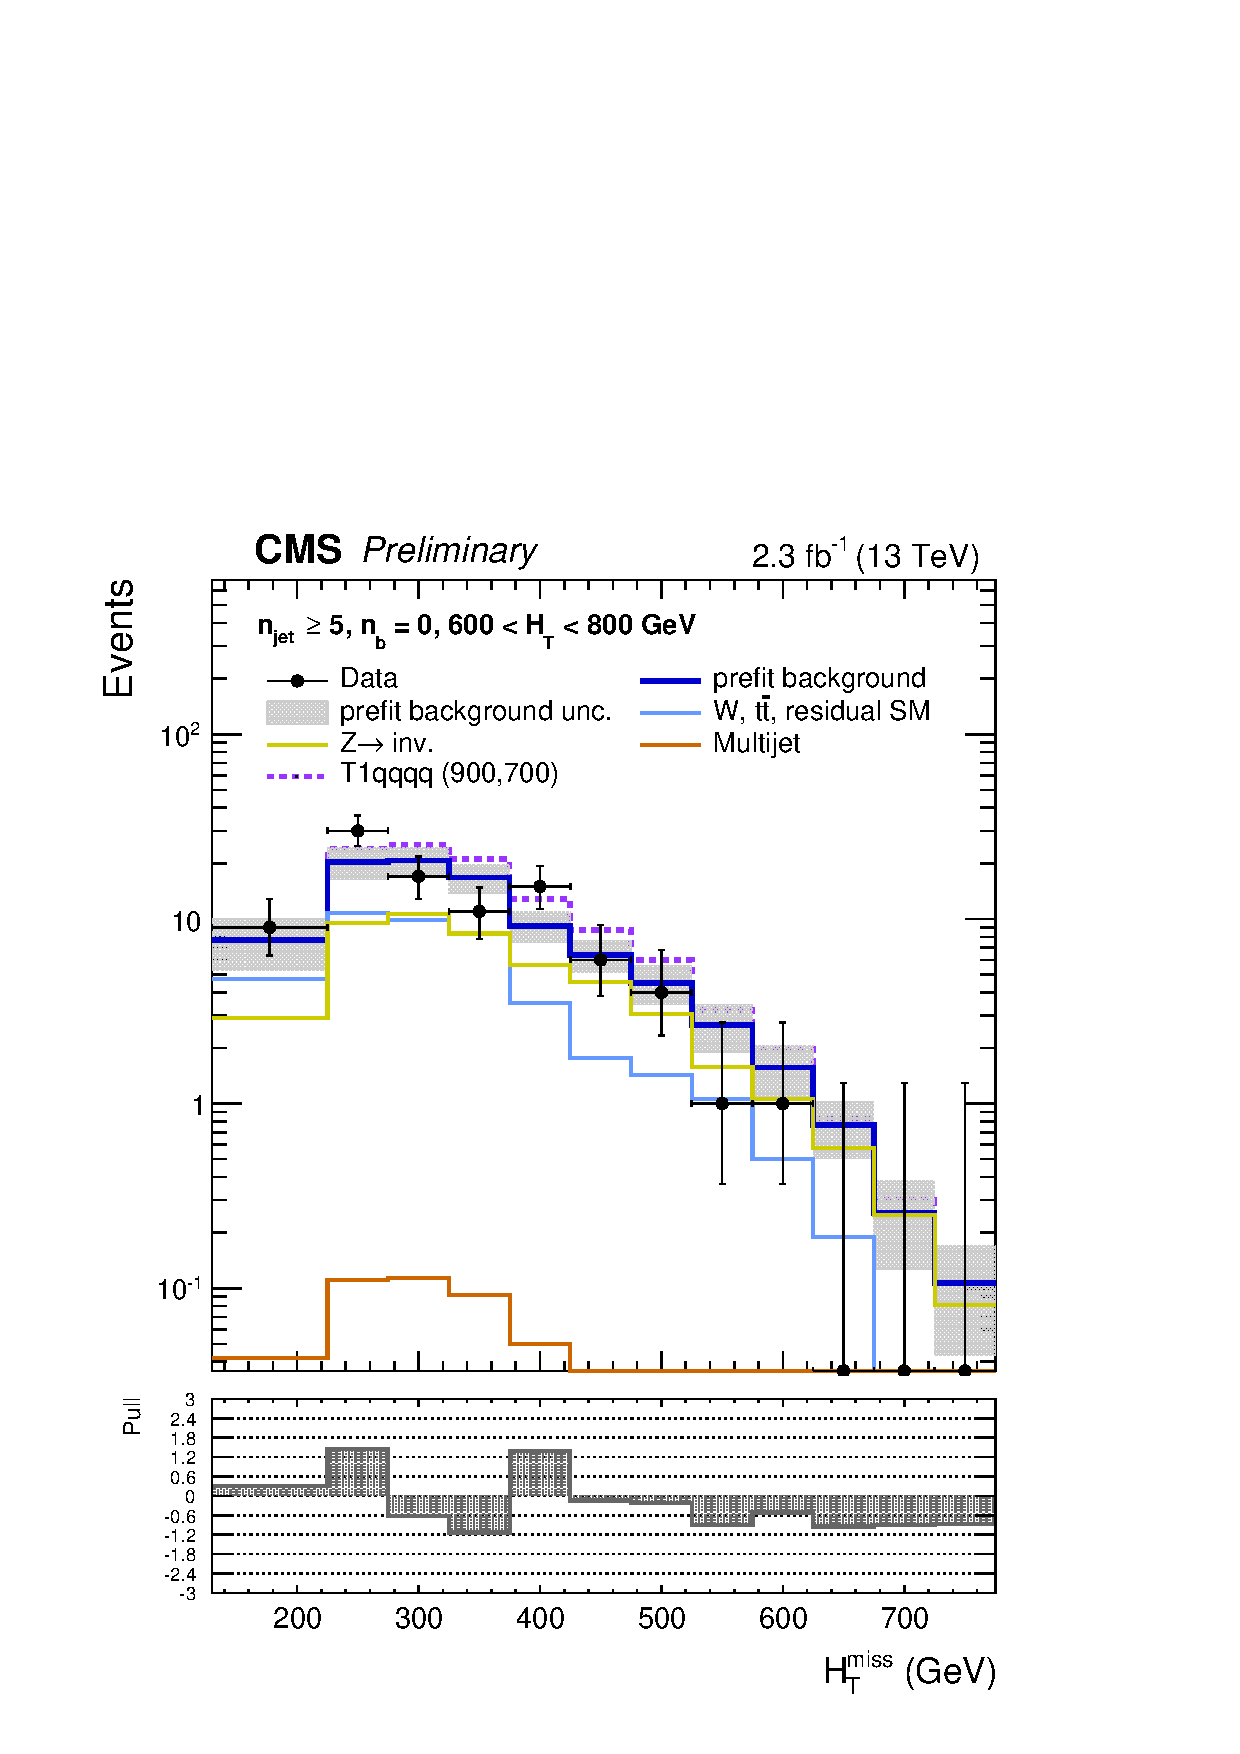
\includegraphics[width=0.45\textwidth]{figures/mht_shapes/v0/postFitShape_eq0b_ge5j_600_800_prefit_T1qqqq_900_700}
    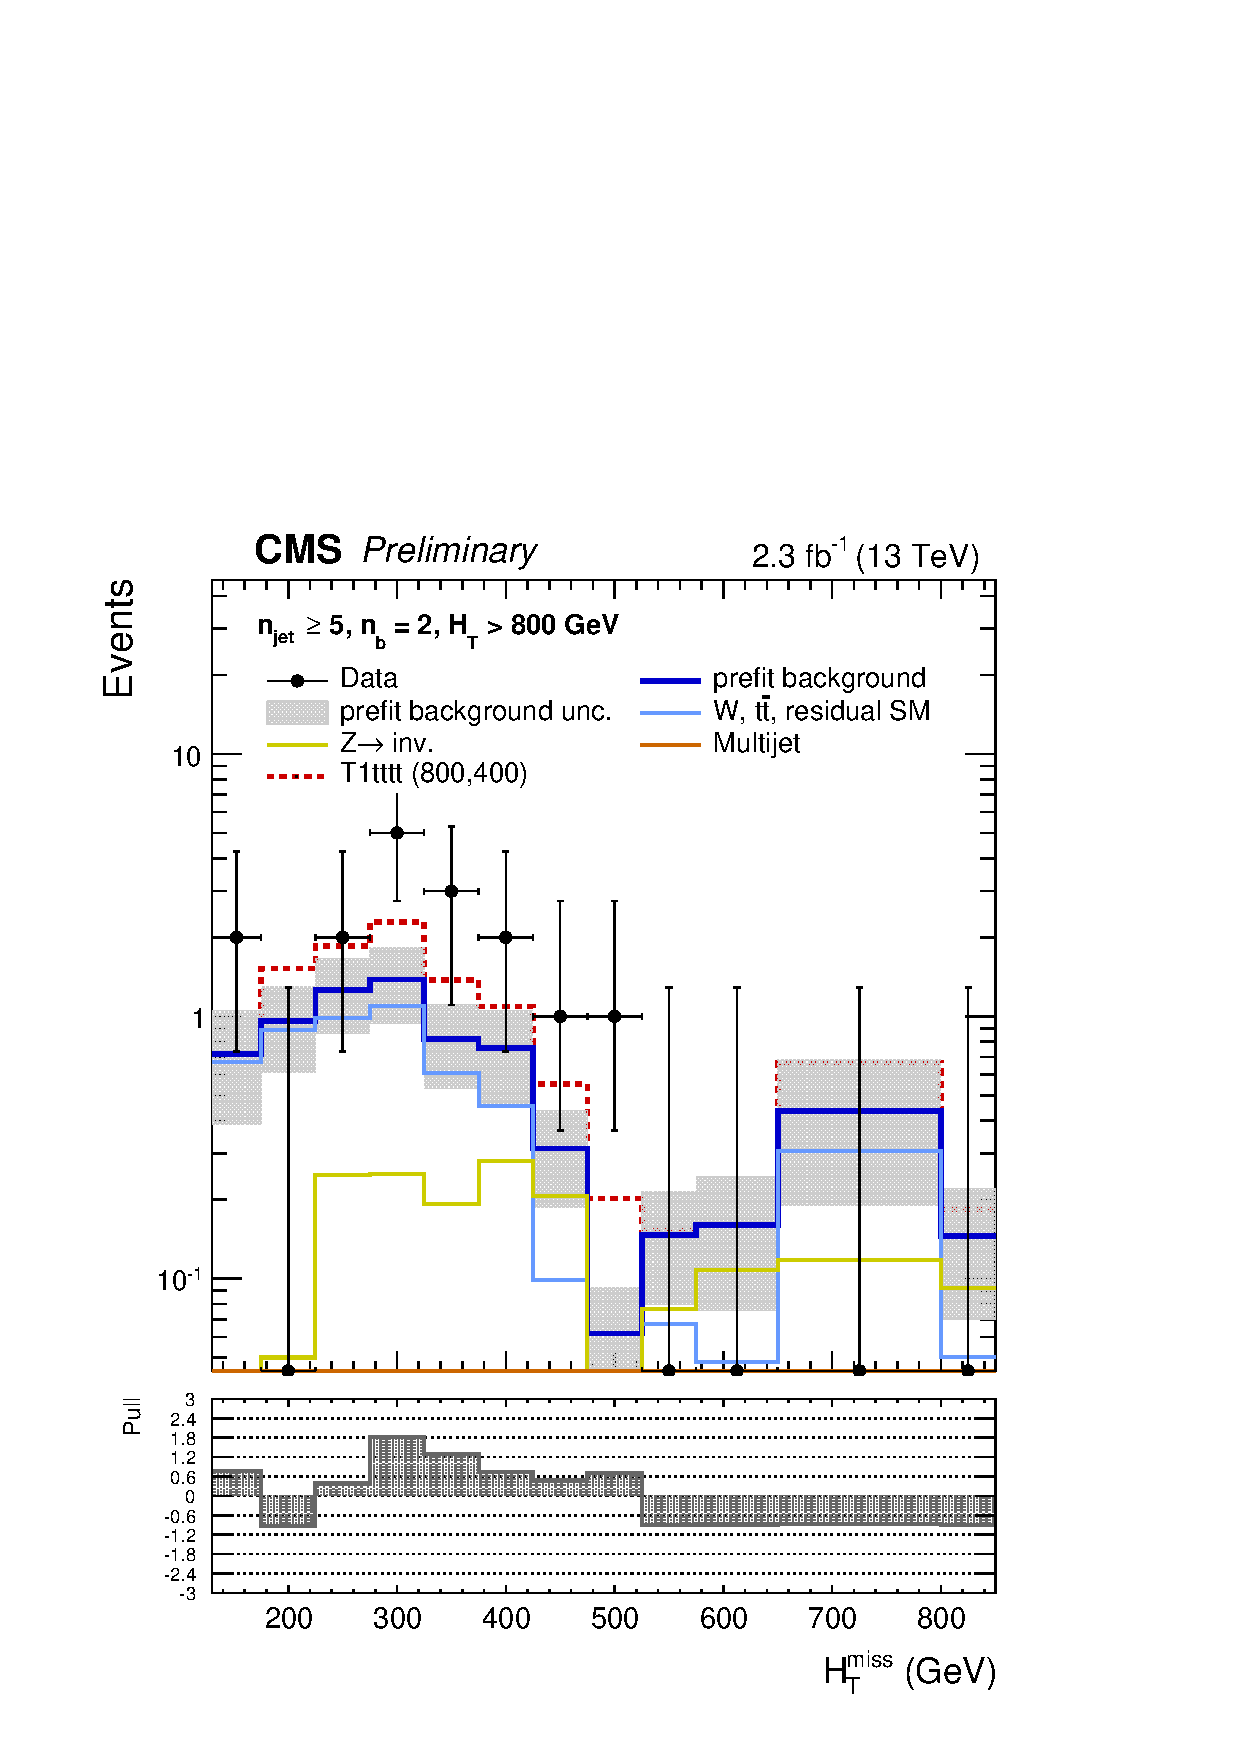
\includegraphics[width=0.49\textwidth]{figures/mht_shapes/v0/postFitShape_eq2b_ge5j_800_Inf_prefit_T1tttt_800_400} 
    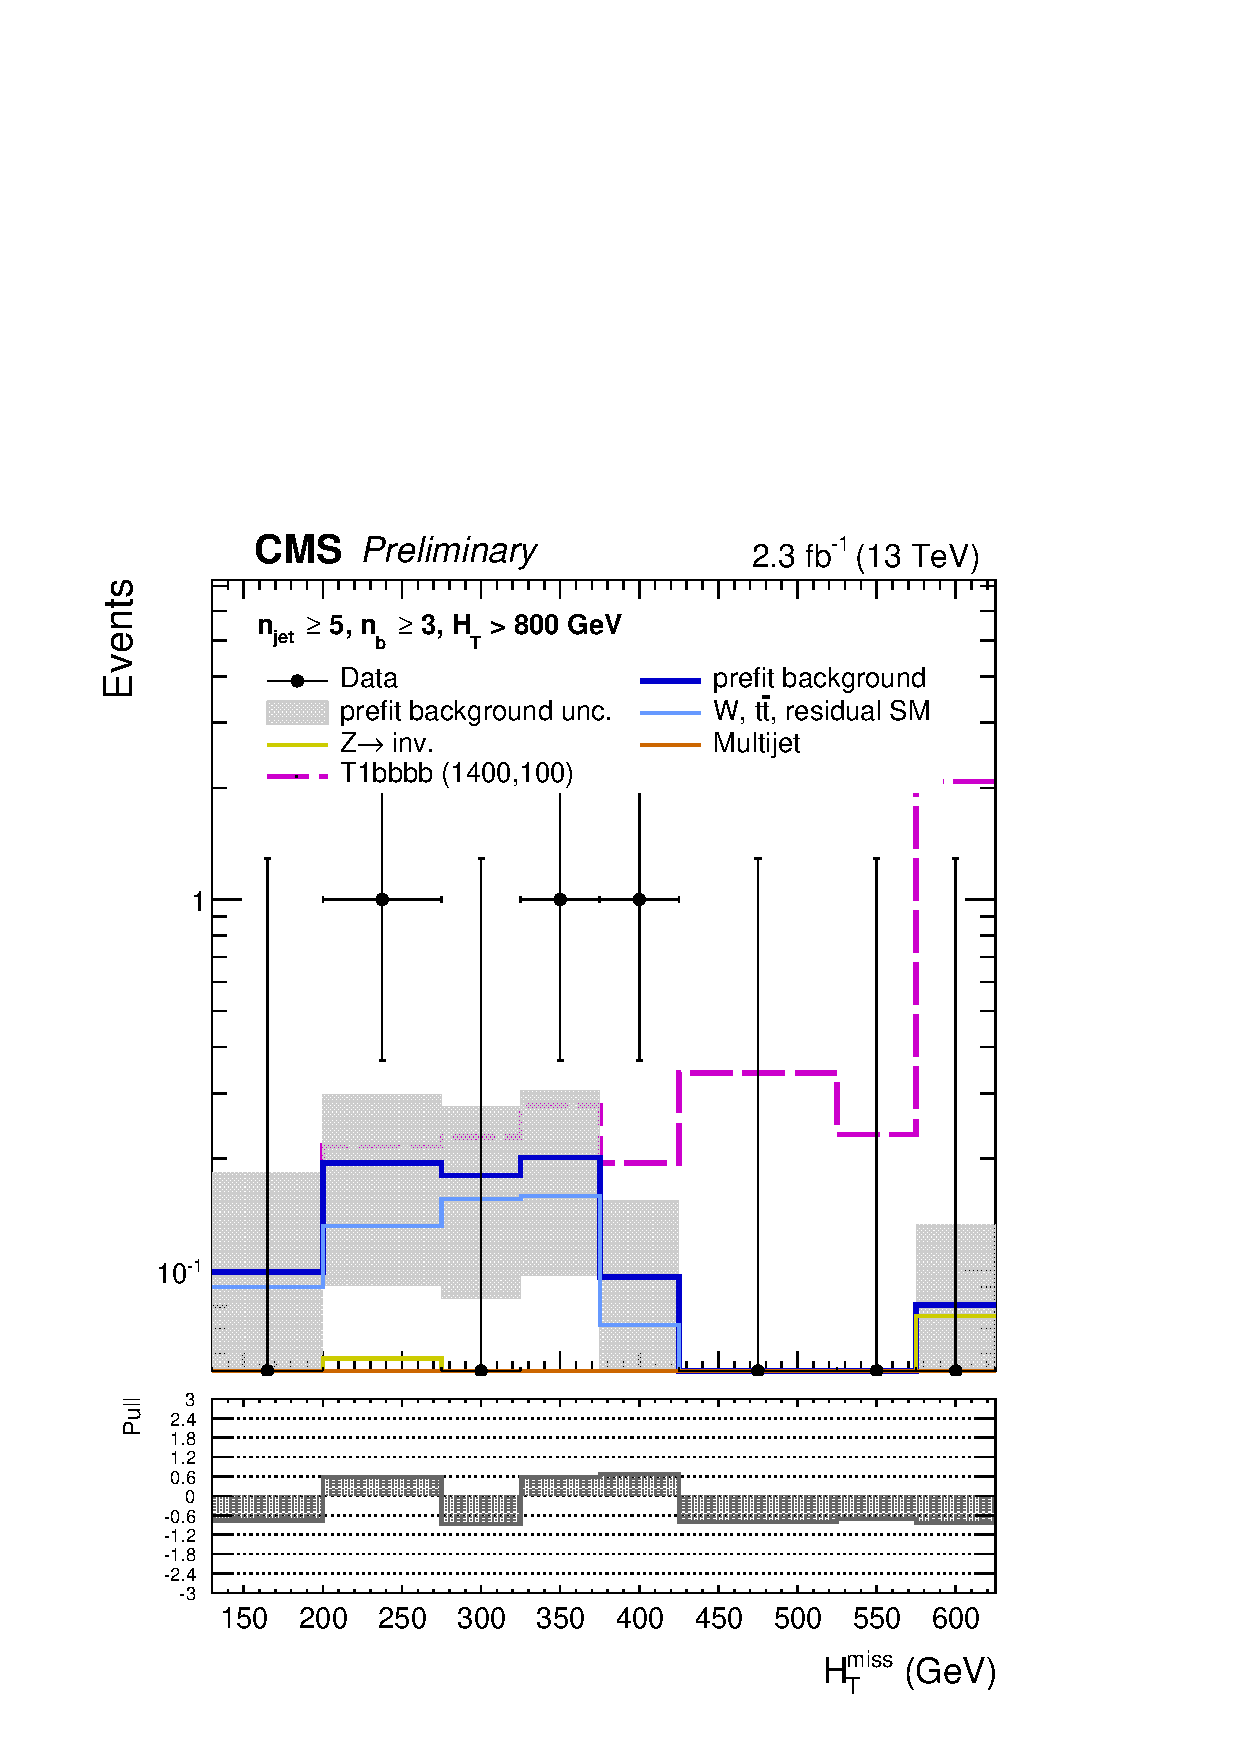
\includegraphics[width=0.49\textwidth]{figures/mht_shapes/v0/postFitShape_ge3b_ge5j_800_Inf_prefit_T1bbbb_1400_100} \\
  \end{center}
  \caption{ The \HTmiss distribution observed in data and the expected
    distribution for the sum of all SM background processes in three 
    representative event categories at high \scalht. The expected
    distributions for example benchmark models with different final state 
    particles and different mass splitting between the gluino and LSP 
    are also shown. \label{fig:mht-templates} }
\end{figure*}

\section{Interpretations} 

The results of the search are used to constrain simplified
supersymmetric models~\cite{Alwall:2008ag, Alwall:2008va, sms}. Each
model assumes the pair production of gluinos or squarks and their
subsequent prompt decays to SM particles and the LSP ($\chiz_1$) with
a 100\% branching ratio (unless indicated otherwise). The gluino
decays contain intermediate on-shell sparticle states (such as the top
squark, $\PSQt$, or the chargino, $\chipm_1$) for a subset of the
models. All other sparticles are assumed to be too heavy ($m_{\sGlu} /
m_{\PSQ} = 5\TeV$) to be produced directly. Three-body decays of
gluinos are assumed to occur via off-shell squarks of light or heavy
flavour. All SM particles with a finite lifetime, such as the W boson,
are assumed to decay naturally. 

\begin{table*}[tb]
  \topcaption{A summary of the simplified models used in this
    analysis. All on-shell sparticles in the decay are stated.}
  \label{tab:simplified-models}
  \centering
  \footnotesize
  \begin{tabular}{ llll }
    \hline
Topology               & Fig.
%                       & Production
                       & Decay
                       & Additional assumptions                                                         \\ [0.5ex]
\hline
\multicolumn{4}{l}{\it Gluino-mediated and direct production of light-flavour squarks}       \\ [0.5ex]
\texttt{T1qqqq}        %& \ref{fig:T1qqqq_feyn}                                                  
                       & $\text{pp}\ra\sGlu\sGlu$
                       & $\sGlu\ra\cPaq\cPq\chiz_1$
                       & --                                                                             \\ [0.5ex]
\texttt{T2qq\_8fold}   %& \ref{fig:T2qq_feyn}                     
                       & $\text{pp}\ra\PSQ\PASQ$        
                       & $\PSQ\ra\cPq\chiz_1$
                       & $m_{\PSQ} = m_{\PSQ_\cmsSymbolFace{L}} = m_{\PSQ_\cmsSymbolFace{R}}$,
                       $\PSQ = \{ \PSQu, \PSQd, \PSQs, \PSQc \}$                                        \\ [0.5ex]
\texttt{T2qq\_1fold}   %& \ref{fig:T2qq_feyn}                                                  
                       & $\text{pp}\ra\PSQ\PASQ$         
                       & $\PSQ\ra\cPq\chiz_1$
                       & $m_{\PSQ (\PSQ \neq \PSQu_\cmsSymbolFace{L})} \gg m_{\PSQu_\cmsSymbolFace{L}}$ \\ [0.5ex]
\multicolumn{4}{l}{\it Gluino-mediated production of off-shell third-generation squarks}               \\ [0.5ex]
\texttt{T1bbbb}        %& \ref{fig:T1bbbb_feyn}                                                   
                       & $\text{pp}\ra\sGlu\sGlu$       
                       & $\sGlu\ra\cPaqb\cPqb\chiz_1$
                       & --                                                                             \\ [0.5ex]
\texttt{T1tttt}        %& \ref{fig:T1tttt_feyn}
                       & $\text{pp}\ra\sGlu\sGlu$       
                       & $\sGlu\ra\cPaqt\PSQt^*\ra\cPaqt\cPqt\chiz_1$
                       & --                                                                             \\ [0.5ex]
\texttt{T1ttbb}        %& \ref{fig:T1ttbb_feyn} 
                       & $\text{pp}\ra\sGlu\sGlu$      
                       & $\sGlu\ra\cPaqt\cPqb\chipm_1\ra\cPaqt\cPqb\PW^*\chiz_1$
                       & $m_{\chipm_1} - m_{\chiz_1} = 5\GeV$                                           \\ [0.5ex]
\multicolumn{4}{l}{\it Natural gluino-mediated production of on-shell top squarks}                     \\ [0.5ex]
\texttt{T5tttt}        %& \ref{fig:T5tttt_feyn}
                       & $\text{pp}\ra\sGlu\sGlu$      
                       & $\sGlu\ra\cPaqt\PSQt\ra\cPaqt\cPqt\chiz_1$ 
                       & $m_{\,\PSQt} - m_{\chiz_1} = 175\GeV$                                          \\ [0.5ex]
\texttt{T5ttcc}        %& \ref{fig:T5ttcc_feyn}            
                       & $\text{pp}\ra\sGlu\sGlu$       
                       & $\sGlu\ra\cPaqt\PSQt\ra\cPaqt\cPqc\chiz_1$ 
                       & $m_{\,\PSQt} - m_{\chiz_1} = 20\GeV$                                           \\ [0.5ex]
\texttt{T5tttt\_degen} %& \ref{fig:T5tttt_degen_feyn}
                       & $\text{pp}\ra\sGlu\sGlu$      
                       & $\sGlu\ra\cPaqt\PSQt\ra\cPaqt\cPqb\PW^*\chiz_1$
                       & $m_{\,\PSQt} - m_{\chiz_1} = 20\GeV$                                           \\ [0.5ex]
\multicolumn{4}{l}{\it Direct production of on-shell third-generation squarks}                         \\ [0.5ex]
\texttt{T2bb}          %& \ref{fig:T2bb_feyn}
                       & $\text{pp}\ra\PSQb\PASQb$     
                       & $\PSQb\ra\cPqb\chiz_1$
                       & --                                                                             \\ [0.5ex]
\texttt{T2tb}          %& \ref{fig:T2tb_feyn}
                       & $\text{pp}\ra\PSQt\PASQt$     
                       & $\PSQt\ra\cPqt\chiz_1 \;\text{or}\; \cPqb\chipm_1\ra\cPqb\PW^*\chiz_1$
                       & $\mathcal{BR} = 50/50\%$, $m_{\chipm_1} - m_{\chiz_1} = 5\GeV$                 \\ [0.5ex]
\texttt{T2tt}          %& \ref{fig:T2tt_feyn}
                       & $\text{pp}\ra\PSQt\PASQt$
                       & $\PSQt\ra\cPqt\chiz_1$
                       & --                                                                             \\ [0.5ex]
\texttt{T2cc}          %& \ref{fig:T2cc_feyn}
                       & $\text{pp}\ra\PSQt\PASQt$      
                       & $\PSQt\ra\cPqc\chiz_1$
                       & $10 < m_{\,\PSQt} - m_{\chiz_1} < 80\GeV$                                      \\ [0.5ex]
\texttt{T2tt\_degen}   %& \ref{fig:T2tt_degen_feyn}
                       & $\text{pp}\ra\PSQt\PASQt$      
                       & $\PSQt\ra\cPqb\PW^*\chiz_1$
                       & $10 < m_{\,\PSQt} - m_{\chiz_1} < 80\GeV$                                      \\ [0.5ex]
\texttt{T2tt\_mixed}   %& \ref{fig:T2tt_mixed_feyn}
                       & $\text{pp}\ra\PSQt\PASQt$      
                       & $\PSQt\ra\cPqc\chiz_1 \;\text{or}\; \cPqb\PW^*\chiz_1$
                       & $\mathcal{BR} = 50/50\%$, $10 < m_{\,\PSQt} - m_{\chiz_1} < 80\GeV$            \\ [0.5ex]
    \hline
  \end{tabular}
\end{table*}

Fifteen unique production and decay modes are considered, which yield
a range of topologies and final states (with only the all-jet final
state considered in this search). Scans in the gluino or squark
($m_{\sGlu} / m_{\PSQ}$) and LSP ($m_{\chiz_1}$) mass parameter space
are performed for each model. Each class of simplified model is
identified by a label that indicates the topology and final state, and
the production and decay mode is indicated by the diagrams shown in
Fig.~\ref{fig:simplified-models}. Table~\ref{tab:simplified-models}
summarises the production and decay modes, as well as any additional
assumptions that define each simplified model. The models can be
categorised according to the following descriptions: the
gluino-mediated and direct production of light-flavour squarks; the
gluino-mediated production of off-shell third-generation squarks; the
``natural'' gluino-mediated production of on-shell top squarks; and
the direct production of on-shell third-generation squarks. In the
case of direct pair production of light-flavour squarks, two different
assumptions on the theory production cross section are made. For the
``eightfold'' scenario (\texttt{T2qq\_8fold}), the scalar partners to
left- and right-handed quarks of the u, d, s, and c flavours are
assumed to be light and degenerate in mass, with other squark states
decoupled to a high mass. For the ``onefold'' scenario
(\texttt{T2qq\_1fold}), only a single light squark is assumed to
particate in the interaction and all other squarks are decoupled to a
high mass. 

Under the background + signal hypothesis, and in the presence of a
non-zero signal contribution, a modified frequentist approach is used
to determine upper limits at 95\% confidence level (CL) on the cross
section, $\sigma_\text{UL}$ (pb), to produce pairs of supersymmetric
particles as a function of the parent sparticle and the LSP
masses. The potential contributions from a new-physics signal to each
of the signal and control regions are considered, even though the only
significant contribution occurs in the signal region and not the
control region (\ie signal contamination). The approach is based on
the one-sided (LHC-style) profile likelihood ratio as the test
statistic, the \cls criterion~\cite{junk, read}, and asymptotic
formulae~\cite{Cowan:2010js} are utilised to approximate the
distributions of the test statistics under the SM background-only and
signal + background hypotheses.
%The test statistic is $q_\mu = -2 \ln (\mathcal{L}_\mu /
%\mathcal{L}_\text{max})$, where $\mathcal{L}_\text{max}$ is the
%maximum likelihood determined by allowing all parameters including a
%multiplier $\mu$ on the production cross section (``signal strength'')
%to vary, and $\mathcal{L}_\mu$ is the maximum likelihood for a fixed
%signal strength. To set limits, we use asymptotic results for the test
%statistic [71] and the CLs method described in Refs. [72, 73]. More
%details are provided in Refs. [15, 74].

\begin{table*}[tb]
  \topcaption{Signal efficiency and list of the 4 most excluding jet
    multiplicity categories for compressed and uncompressed models
    used in the analysis. }
  \label{tab:signal-eff}
  \centering
  \begin{tabular}{ lllcrrrrrcc }
    \hline
    \multicolumn{2}{l}{Benchmark models} 
  & Most sensitive
  & $\mathcal{A}\times\varepsilon$
  & \multicolumn{4}{c}{Systematic uncertainties [\%]}
  & $\sigma_\text{theory}$
  & \multicolumn{2}{c}{$\mu$ (95\% CL)}                                                                         \\ [0.3ex]
    \cline{5-8}
    \multicolumn{2}{l}{$(m_{\text{SUSY}}, m_{\mathrm{LSP}})$ [GeV]} 
  & \njet categories
  & [\%]    
  & MC stat.
  & ISR 
  & JEC
  & $\text{SF}_\text{b-tag}$
  & \multicolumn{1}{c}{[fb]}
  & Exp.
  & Obs.                                                                                                        \\ [0.3ex] 
    \hline
    \multirow{2}{*}{\texttt{T1qqqq}} 
  & (1300, 100) & $\geq$5, 4, 3, 2         & \phantom{1}9.4 & 7-30  & 2-2   & 4-21  & 2-14 & 46.1 & 0.79 & 0.76 \\
  & (900, 700)  & $\geq$5, $\geq$5a, 4, 4a & \phantom{1}5.6 & 10-33 & 1-13  & 1-26  & 1-10 & 677  & 0.58 & 0.44 \\ [0.5ex]
    \multirow{2}{*}{\texttt{T2qq\_8fold}}
  & (1050, 100) & $\geq$5, 3, 2, 4         & 13.4           & 7-33  & 2-5   & 3-16  & 1-11 & 44.0 & 0.72 & 0.50 \\
  & (650, 550)  & $\geq$5, 4, $\geq$5a, 4a & \phantom{1}2.6 & 10-28 & 3-9   & 2-28  & 1-6  & 1080 & 0.74 & 0.64 \\ [0.5ex]
     \multirow{2}{*}{\texttt{T2qq\_1fold}}
  & (1050, 100) & $\geq$5, 3, 2, 4         & 17.9           & 7-33  & 2-5   & 3-16  & 1-11 & 44.0 & 0.72 & 0.50 \\
  & (650, 550)  & $\geq$5, 4, $\geq$5a, 4a & \phantom{1}2.6 & 10-28 & 3-9   & 2-28  & 1-6  & 1080 & 0.74 & 0.64 \\ [0.5ex]
    \multirow{2}{*}{\texttt{T1bbbb}}
  & (1500, 100) & $\geq$5, 4, 3, 2         & 10.1           & 5-17  & 1-2   & 1-12  & 2-22 & 14.2 & 0.81 & 0.79 \\
  & (1000, 800) & $\geq$5, 4, $\geq$5a, 4a & \phantom{1}4.9 & 8-31  & 1-17  & 1-40  & 1-14 & 325  & 0.33 & 0.32 \\ [0.5ex]
    \multirow{2}{*}{\texttt{T1tttt}}
  & (1300, 100) & $\geq$5, $\geq$5a, 4, 3  & \phantom{1}2.4 & 7-16  & 1-2   & 2-7   & 2-12 & 46.1 & 1.00 & 1.89 \\
  & (800, 400)  & $\geq$5, $\geq$5a, 4, 4a & \phantom{1}0.6 & 7-27  & 1-2   & 3-45  & 1-8  & 1490 & 0.56 & 1.03 \\ [0.5ex]
    \multirow{2}{*}{\texttt{T1ttbb}}
  & (1300, 100) & $\geq$5, 4, 3, $\geq$5a  & \phantom{1}3.8 & 9-32  & 1-2   & 3-16  & 2-19 & 46.1 & 0.60 & 0.91 \\
  & (1000, 700) & $\geq$5, $\geq$5a, 4, 3  & \phantom{1}3.4 & 9-30  & 1-9   & 3-65  & 1-14 & 325  & 0.51 & 0.70 \\ [0.5ex]
    \multirow{2}{*}{\texttt{T5tttt}}
  & (800, 100)  & $\geq$5, $\geq$5a, 3, 4  & \phantom{1}0.2 & 12-20 & 2-4   & 3-5   & 1-6  & 1490 & 0.69 & 1.19 \\
  & (700, 400)  & $\geq$5, $\geq$5a, 4, 4a & \phantom{1}0.2 & 20-29 & 2-10  & 8-10  & 1-2  & 3530 & 1.00 & 1.35 \\ [0.5ex]
% & (700, 400)  & $\geq$5, $\geq$5a, 4, 4a & \phantom{1}0.2 & 20-20 & 2-10  & 10-10 & 2-2  &      & 1.00 & 1.35 \\ [0.5ex]
% T5ttttDM175 (700,400)
%  Efficiency      0.2   0.3
%  isrSignalWeight 1.0   10.0
%  jecWeight       8.0   62.0
%  puWeight        1.0   22.0
%  bsfWeight       1.0   23.0
%  triggerWeight   6.0   19.0
%  mcStat          29.0  50.0
    \multirow{2}{*}{\texttt{T5ttcc}}  
  & (1200, 200) & $\geq$5, 4, 3, $\geq$5a  & \phantom{1}4.9 & 6-25  & 5-25  & 3-21  & 1-24 & 85.6 & 0.58 & 0.87 \\
  & (750, 600)  & $\geq$5, $\geq$5a, 4, 4a & \phantom{1}1.0 & 9-23  & 1-4   & 5-21  & 1-3  & 2270 & 0.89 & 0.72 \\ [0.5ex]
    \multirow{2}{*}{\texttt{T5tttt\_degen}} 
  & (1100, 100) & $\geq$5, 4, 3, 4a        & \phantom{1}1.3 & 15-21 & 12-16 & 6-11  & 4-15 & 16.3 & 0.89 & 2.55 \\
  & (800, 600)  & $\geq$5, $\geq$5a, 4a, 4 & \phantom{1}1.9 & 5-32  & 1-8   & 1-34  & 1-7  & 1490 & 0.66 & 0.70 \\ [0.5ex]
    \multirow{2}{*}{\texttt{T2bb}}
  & (800, 50)   & 2, 3, 4, $\geq$5         & \phantom{1}1.5 & 5-31  & 2-6   & 1-21  & 1-23 & 28.3 & 0.96 & 1.06 \\
  & (375, 300)  & $\geq$5, 4, 3a, 3        & \phantom{1}0.1 & 8-33  & 1-10  & 3-25  & 1-7  & 2610 & 0.67 & 0.87 \\ [0.5ex]
    \multirow{2}{*}{\texttt{T2tb}}
  & (600, 50)   & $\geq$5, 4, 3, 2         & \phantom{1}6.1 & 3-28  & 1-3   & 1-22  & 1-17 & 175  & 0.70 & 1.35 \\
  & (350, 225)  & $\geq$5, 4, 3, 3a        & \phantom{1}1.0 & 9-33  & 1-4   & 2-41  & 1-8  & 3790 & 0.79 & 0.88 \\ [0.5ex]
    \multirow{2}{*}{\texttt{T2tt}}
  & (700, 50)   & $\geq$5, 4, 3, $\geq$5a  & \phantom{1}8.1 & 8-33  & 1-4   & 2-22  & 1-21 & 67.0 & 0.90 & 1.19 \\
  & (350, 100)  & $\geq$5, $\geq$5a, 4a, 4 & \phantom{1}1.4 & 7-31  & 1-1   & 1-28  & 1-7  & 3790 & 0.44 & 0.50 \\ [0.5ex]
    \multirow{1}{*}{\texttt{T2cc}}
  & (325, 305)  & $\geq$5, 4, 3, 2         & \phantom{1}0.8 & 3-32  & 1-27  & 1-27  & 1-12 & 5600 & 0.92 & 0.68 \\ [0.5ex]
    \multirow{1}{*}{\texttt{T2\_degen}}
  & (300, 290)  & 3, 4, $\geq$5, 2         & \phantom{1}0.9 & 2-27  & 1-27  & 1-25  & 1-12 & 8520 & 0.56 & 0.41 \\ [0.5ex]
    \multirow{1}{*}{\texttt{T2tt\_mixed}}
  & (300, 250)  & $\geq$5, 4, $\geq$5a, 4a & \phantom{1}0.4 & 3-33  & 1-27  & 1-33  & 1-13 & 8520 & 0.99 & 0.58 \\ [0.5ex]
    \hline
  \end{tabular}
\end{table*}

Table~\ref{tab:signal-eff} summarises the experimental acceptance
times efficiency ($\mathcal{A}\times\varepsilon$) for a number of
benchmark models, each chosen to be near the limit of search
sensitivity. For each topology, typically two different pairs of
parent sparticle and LSP masses ($m_\text{SUSY}, m_\text{LSP}$) are
chosen that are characterised by a large and a smaller (\ie
``compressed'') difference in parent sparticle and LSP masses. The
four most sensitive event categories, defined in terms of \njet, are
used to determine $\sigma_\text{UL}$. The categories used per
benchmark model are listed in Table~\ref{tab:signal-eff}, along with
$\mathcal{A}\times\varepsilon$ determined for these four categories.

The uncertainty in $\mathcal{A}\times\varepsilon$ is evaluated
independently for each model, as a function of ($m_\text{SUSY},
m_\text{LSP}$), and contributions from several sources are
considered. Each source of uncertainty is included in the likelihood
function via alternative shapes to the nominal \HTmiss templates
evaluated from simulated signal events categorised according to \njet,
\nb, and \scalht. Correlations are taken into account where
appropriate, including those relevant to signal contamination in the
control regions. The morphing scheme that interpolates between the
nominal and alternative \HTmiss templates, described in Section~\ref{},
is also used for the simulated signal samples.

In addition to the uncertainty in the integrated luminosity of
4.6\%~\cite{lumi}, the following sources of uncertainty are dominant:
the statistical uncertainty arising from the finite size of simulated
signal samples, the modelling of initial-state radiation (ISR), the
corrections to jet energies (JEC) evaluated in simulation, and the
modelling of scale factors ($\text{SF}_\text{b-tag}$) applied to
simulated event samples that correct for differences in the efficiency
and misidentification probability of b quark jets. The magnitude of
each contribution depends on the model and the masses of the parent
sparticle and LSP. 

The $\mathcal{A}\times\varepsilon$ for models with small mass
splittings (\eg $m_{\PSQ} - m_{\chiz_1} \lesssim m_{\text t}$) is due
in large part to ISR, the modelling of which is evaluated by comparing
the simulated and measured \Pt spectra of the system recoiling against
the ISR jets in \ttbar events, using the technique described in
Ref.~\cite{single-lepton-stop}. The uncertainty can be as large as
$\sim$30\%, and is the dominant systematic uncertainty for systems
with a compressed mass spectrum. Uncertainties in the jet energy
scale, as large as $\sim$40\%, can also be dominant for models
characterised by high jet multiplicities in the final state. The
uncertainties in $\text{SF}_\text{b-tag}$ can be as large as
$\sim$25\%. Table~\ref{tab:signal-eff} summarises these dominant
contributions to the uncertainty in $\mathcal{A}\times\varepsilon$ for
a range of benchmark models. Characteristic values for each model are
expressed in terms of a range that is representative of the values
across all bins of the signal region. The upper bound for each range
may be subject to moderate statistical fluctuations. 

Further uncertainties with subdominant contributions are considered on
a similar footing. The uncertainties in the efficiency of identifying
well-reconstructed, isolated leptons are considered, with a typical
magnitude of $\sim$5\% and treated as anti-correlated between the
signal and control regions. A 5\% uncertainty in the minimum bias
cross section, $\sigma_\text{MB} = 69.0 \pm 3.5\unit{mb}$, is assumed
and propagated through to the reweighting procedure to account for
differences between the simulated and data-derived measurements of the
pileup distributions. Finally, uncertainties in the simulation
modelling of the efficiencies of the trigger strategy employed by the
search are typically $<$10\%. 

The choice of PDF set, or variations therein, predominantly affects
$\mathcal{A}\times\varepsilon$ through changes in the \Pt spectrum of
the system recoil, which is covered by the ISR uncertainty, hence no
additional uncertainty is adopted. Uncertainties in
$\mathcal{A}\times\varepsilon$ due to variations in the
renormalisation and factorisation scales are determined to be
relatively small. In both cases, contributions to the uncertainty in
the theory production cross section are considered.

The upper limits on the signal production cross section are evaluated
at a 95\% CL for each of the aforementioned benchmark models. The
limits are expressed in terms of the signal strength parameter, $\mu$,
which is determined relative to the theory cross section that is
calculated at NLO+NLL accuracy. The limits are summarised in
Table~\ref{tab:signal-eff}. Expected limits on $\mu$ are also listed,
which are determined using an asimov data set. All benchmark models
are disfavoured based on expectations. The observed limits fluctuate
around the expected $\mu$ values, with some models exhibiting a
moderately weaker-than-expected limit due to fluctuations in data, as
discussed below.

\begin{figure*}[!h]
  \begin{center}
    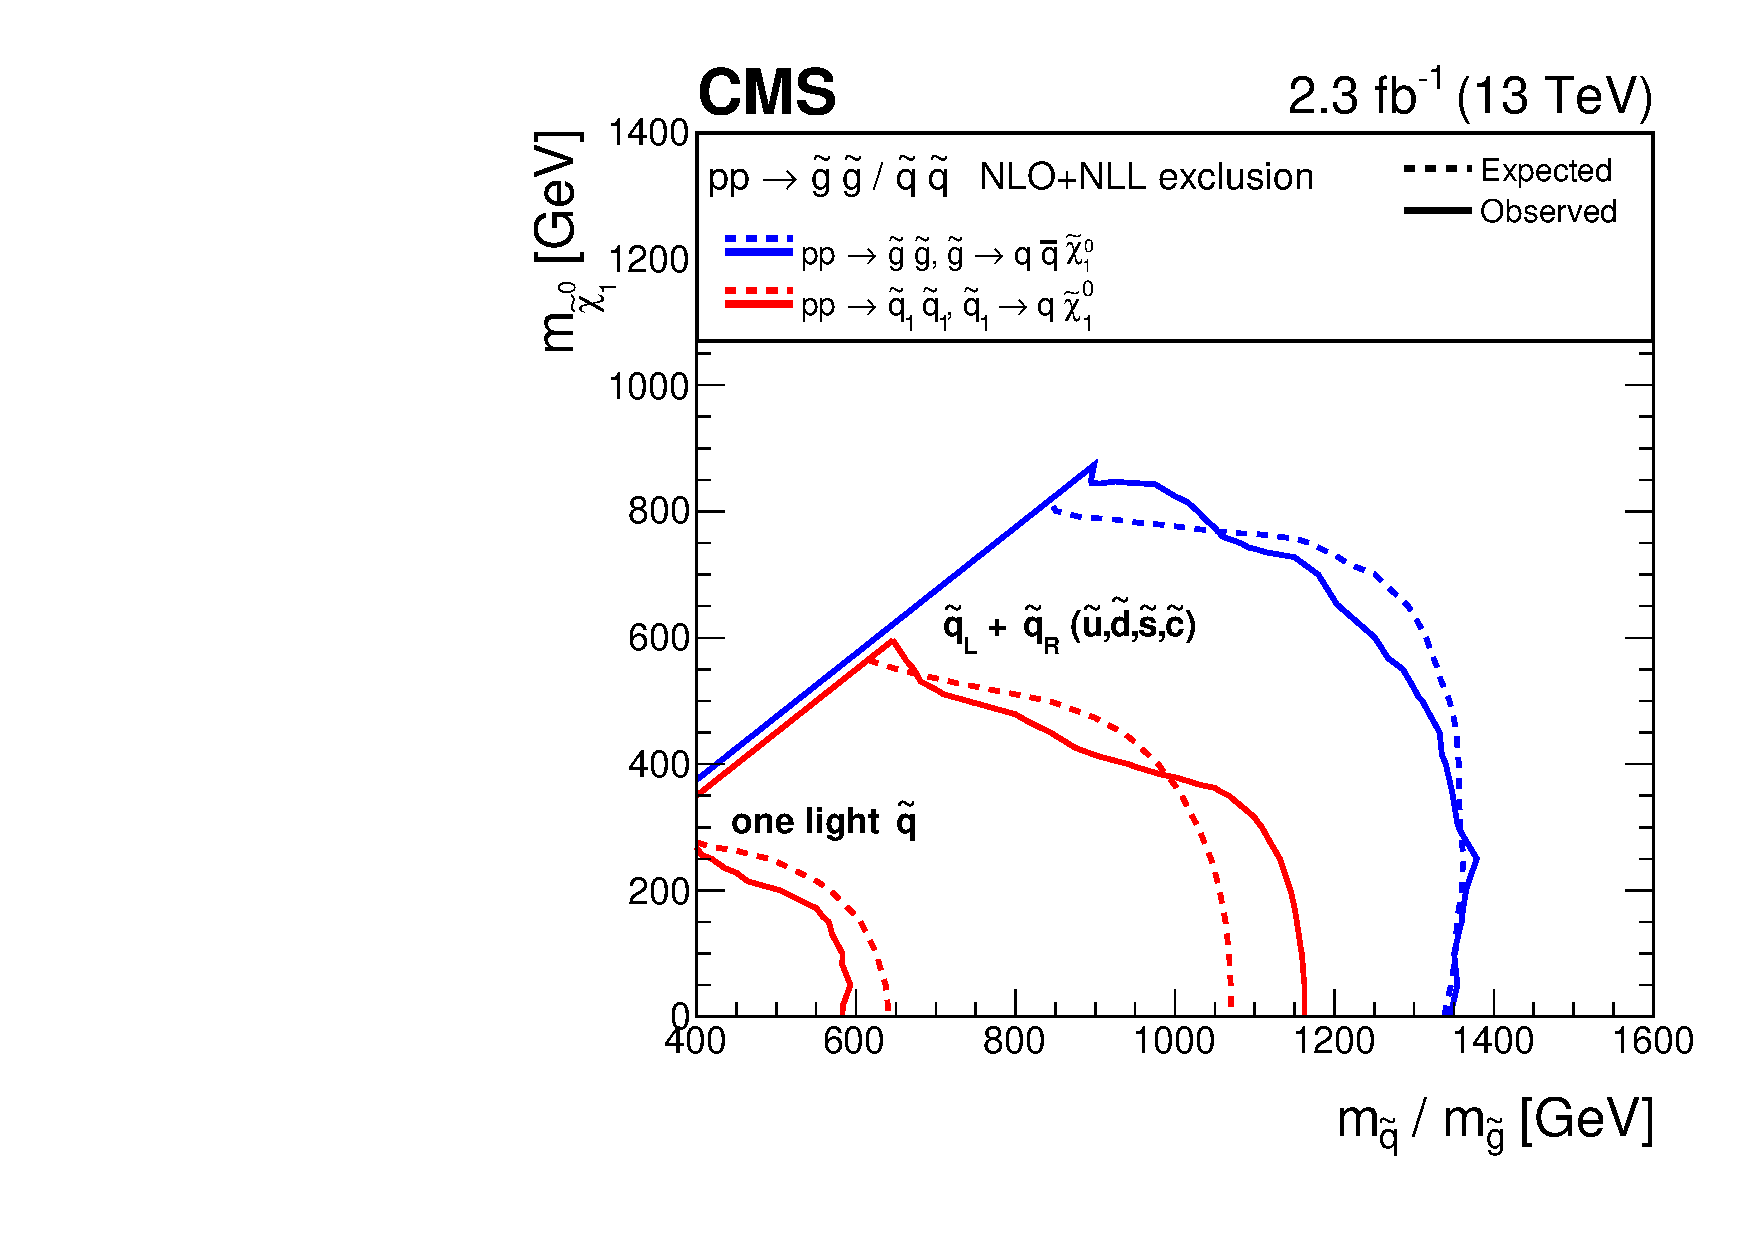
\includegraphics[width=0.6\textwidth]{figures/limits/v1/mixSUMMARY.pdf}
    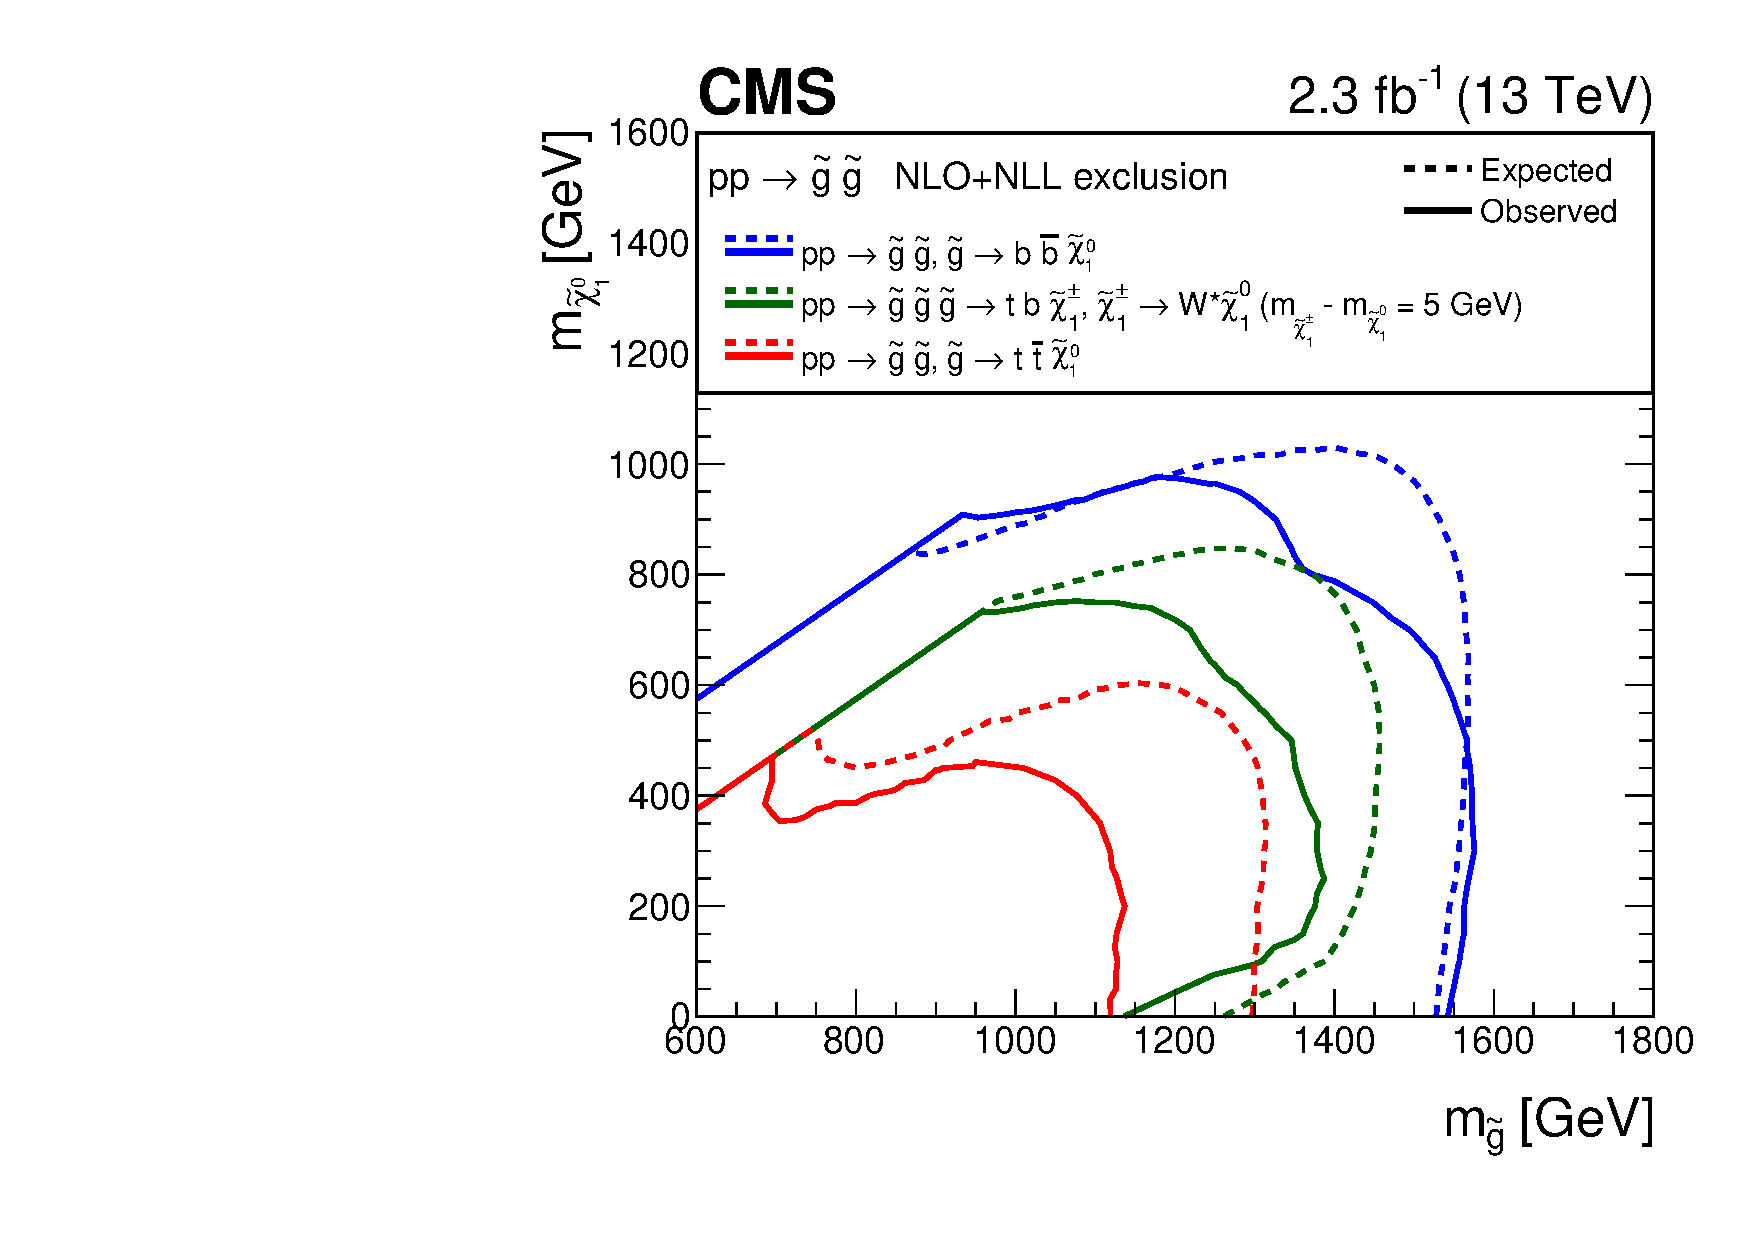
\includegraphics[width=0.6\textwidth]{figures/limits/v1/gluinoSUMMARY.pdf} 
    \caption{Observed upper limit in cross section at 95\% CL
      (indicated by the colour scale) for simplified models that
      assume the pair production of gluinos, as a function of the
      gluino and $\chiz_{1}$ masses for gluino three-body decays to
      $b\bar{b}\chiz_{1}$ (top left), $q\bar{q}\chiz_{1}$ (top right) and $t\bar{t}\chiz_{1}$ (bottom center). 
      The black solid thick (thin) line indicates the observed mass
      exclusion region assuming the nominal (${\pm}1 \sigma$ theory
      uncertainty) production cross section. The red dashed thick
      (thin) line indicates the median (${\pm}1 \sigma$ experimental
      uncertainty) expected exclusion.
    }
    \label{fig:limits-sms-1} 
  \end{center}
\end{figure*}

\begin{figure*}[!h]
  \begin{center}
    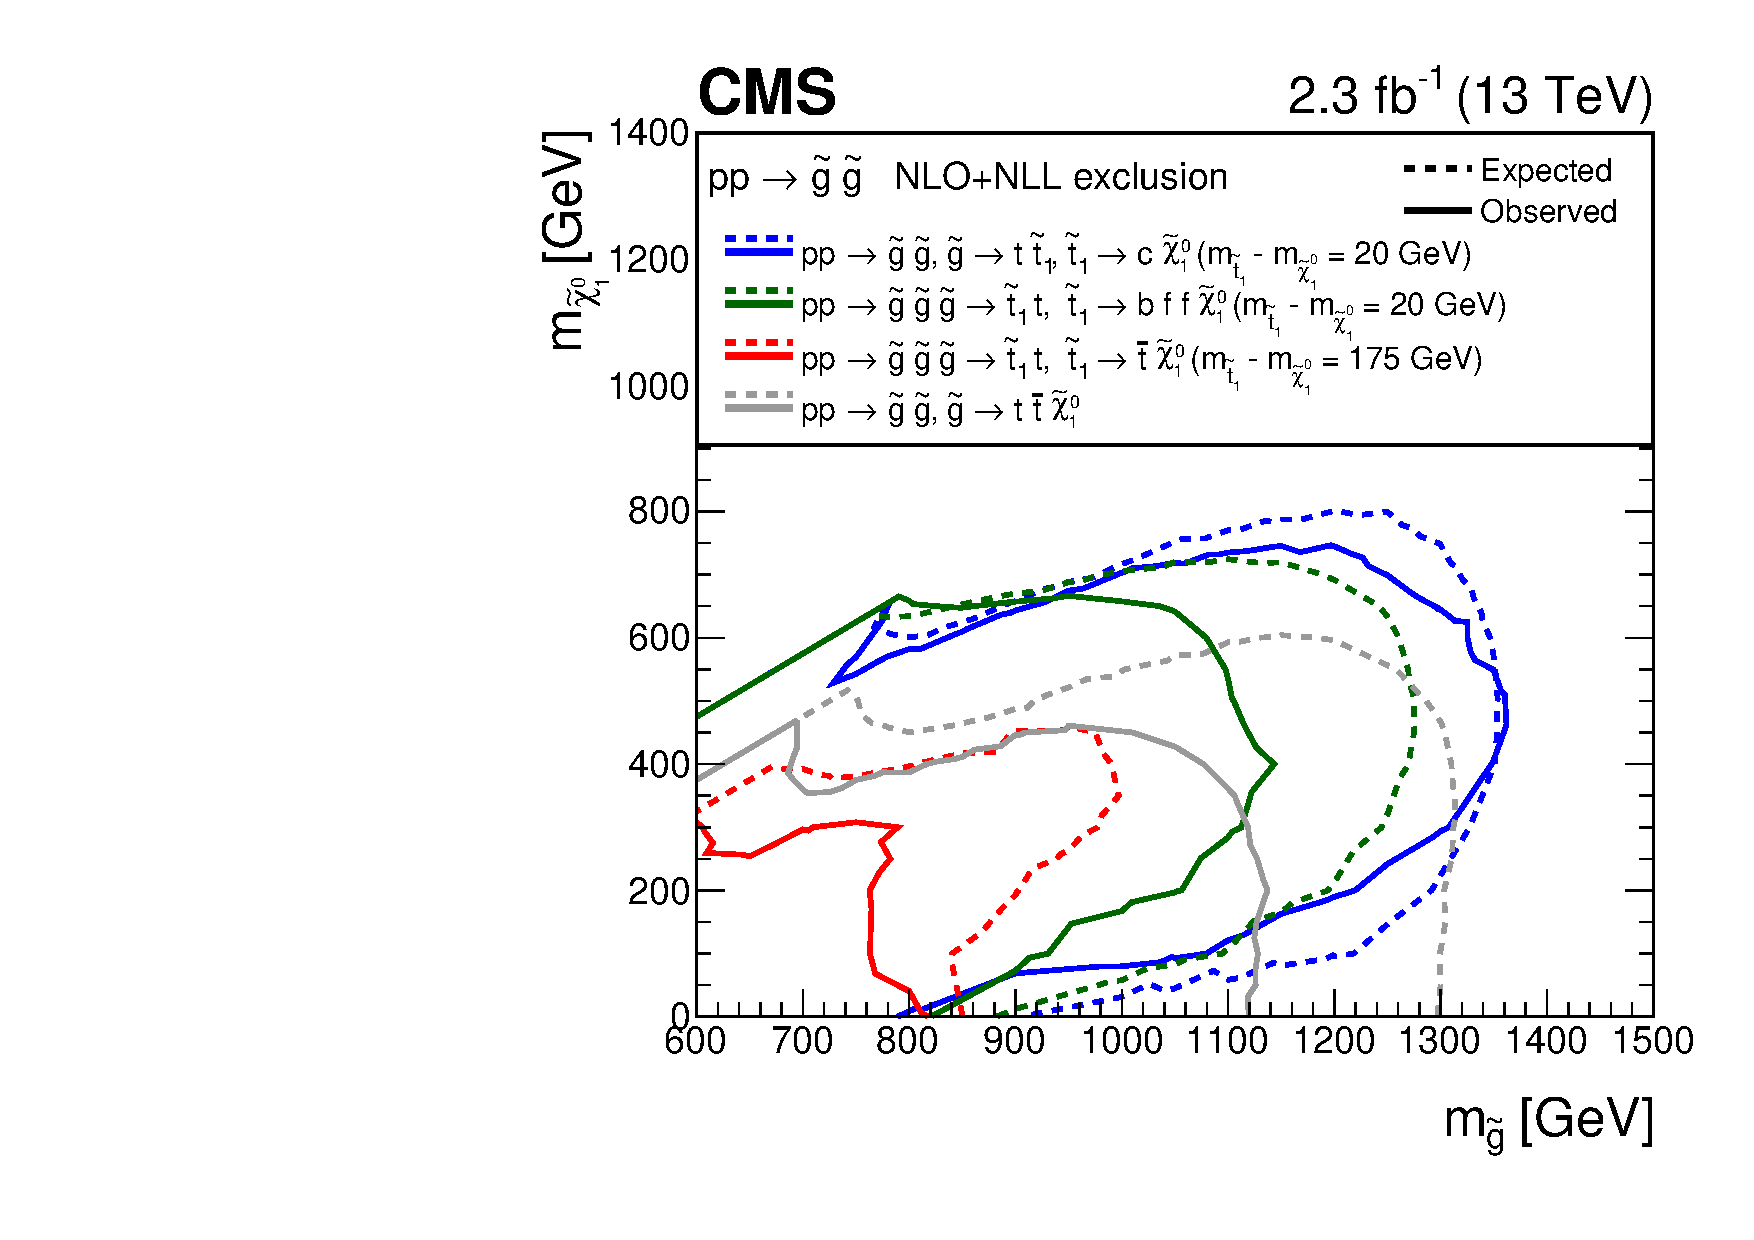
\includegraphics[width=0.6\textwidth]{figures/limits/v1/naturalWT1SUMMARY.pdf}
%    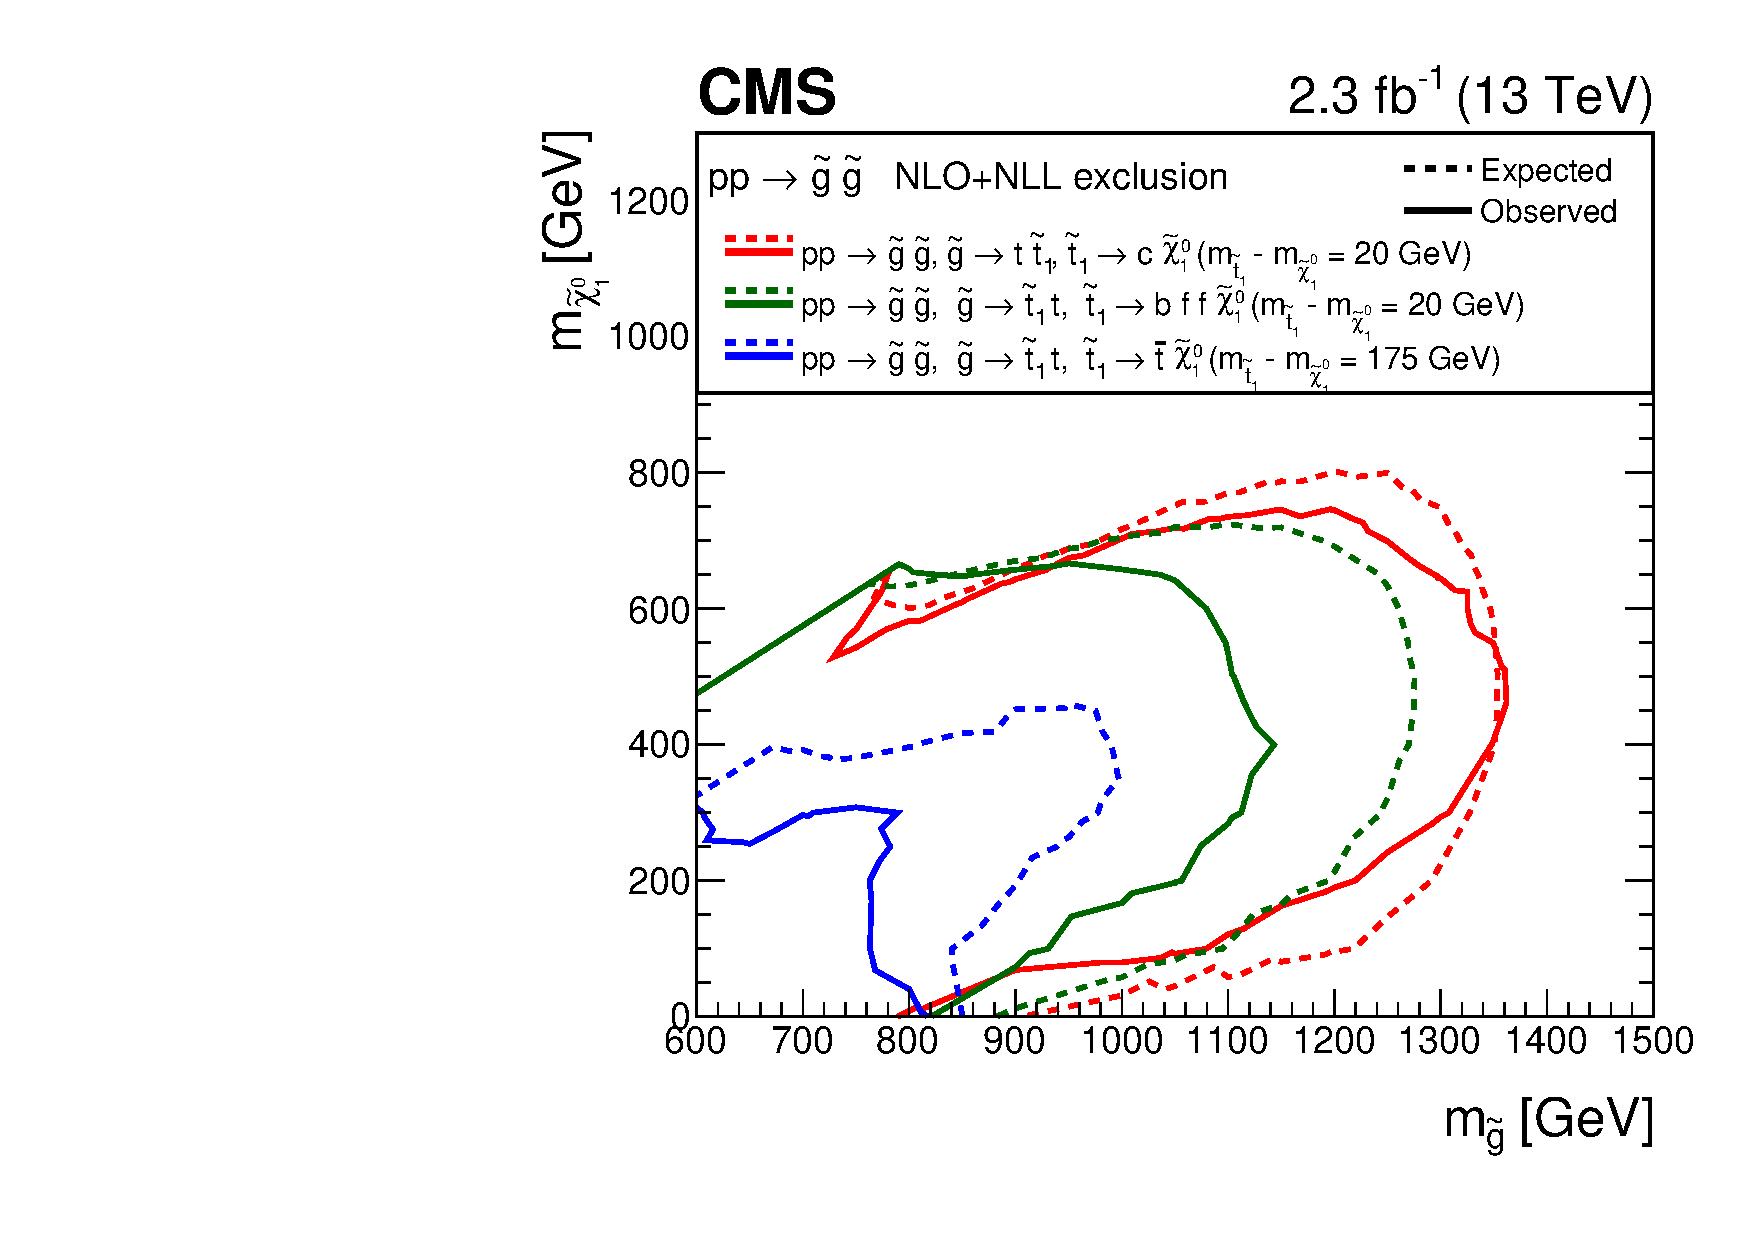
\includegraphics[width=0.6\textwidth]{figures/limits/v1/naturalSUMMARY.pdf}
    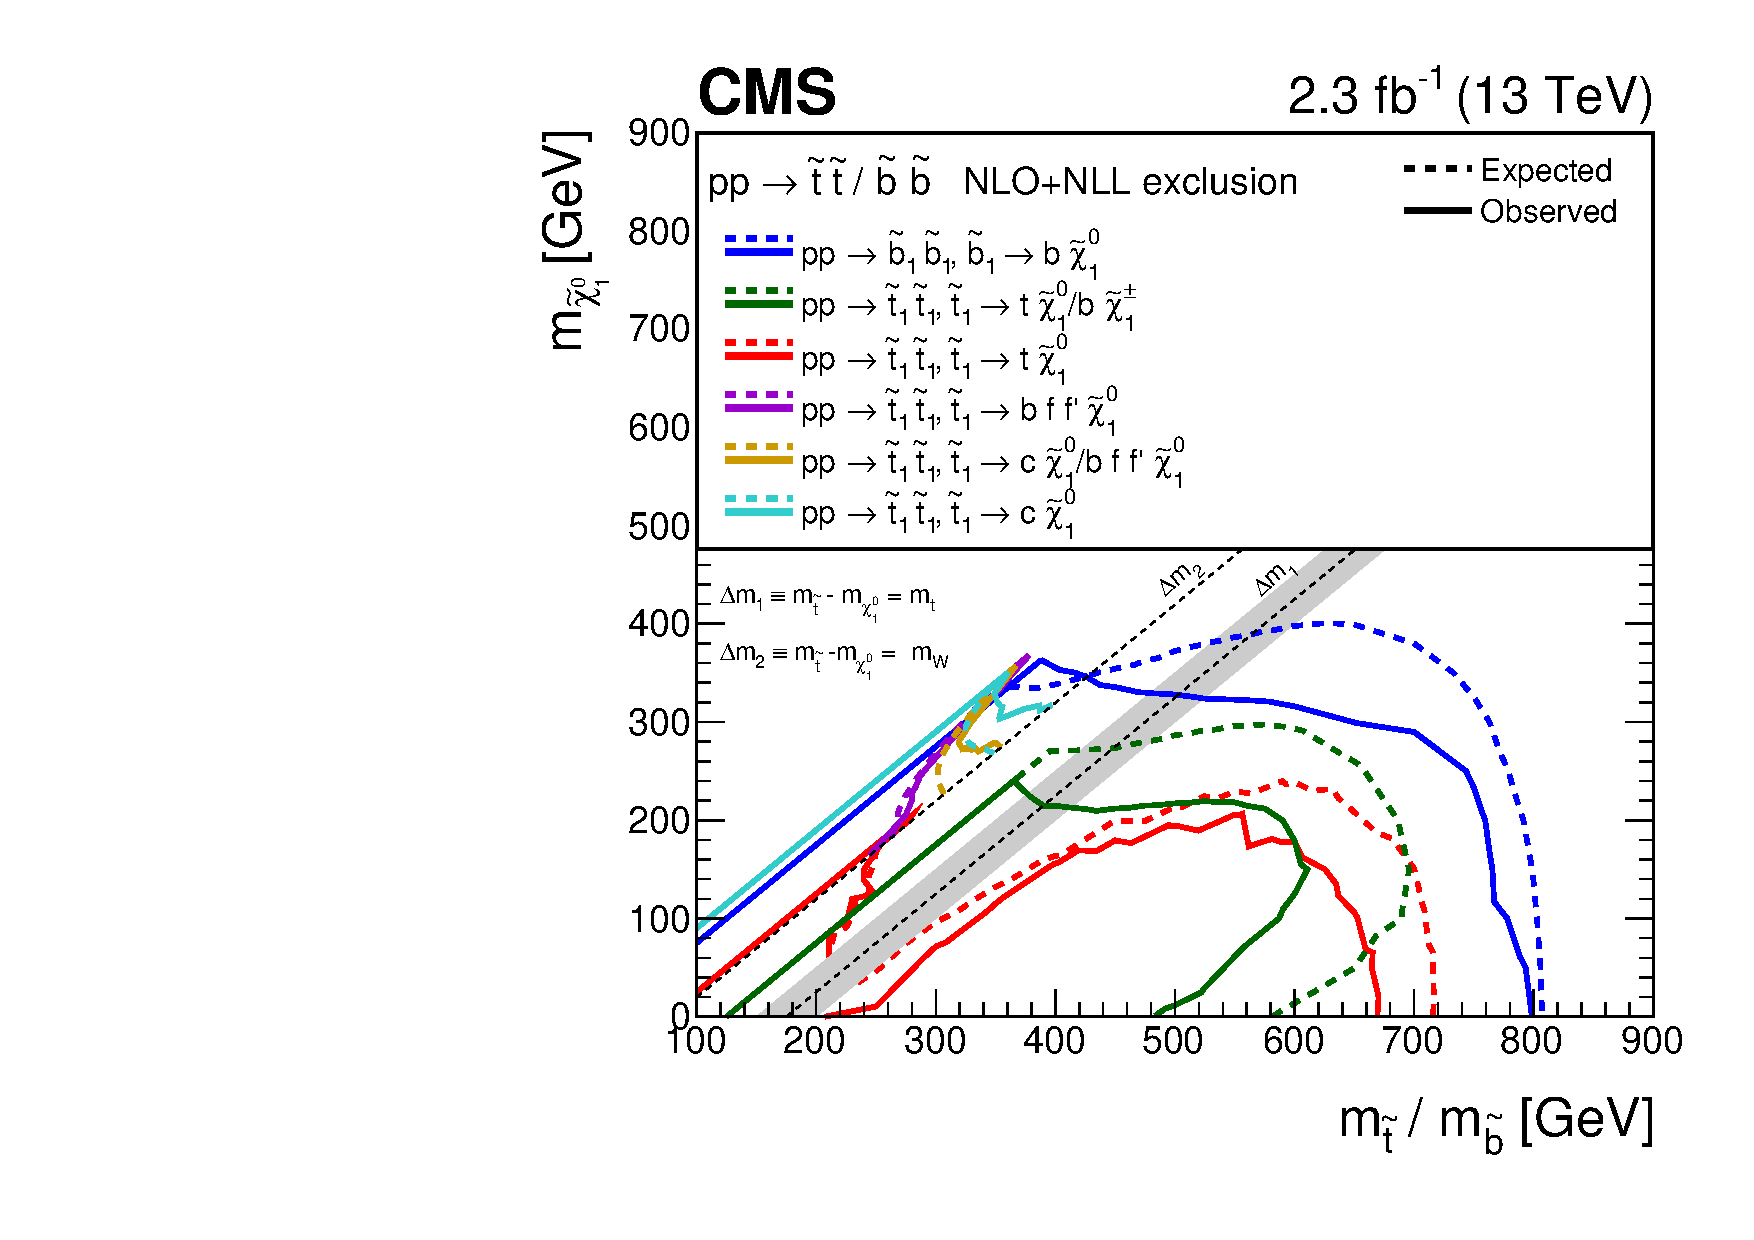
\includegraphics[width=0.6\textwidth]{figures/limits/v1/allThirdGenSUMMARY.pdf} 
    \caption{Observed upper limit in cross section at 95\% CL
      (indicated by the colour scale) for simplified models that
      assume the pair production of gluinos, as a function of the
      gluino and $\chiz_{1}$ masses for gluino three-body decays to
      $b\bar{b}\chiz_{1}$ (top left), $q\bar{q}\chiz_{1}$ (top right) and $t\bar{t}\chiz_{1}$ (bottom center). 
      The black solid thick (thin) line indicates the observed mass
      exclusion region assuming the nominal (${\pm}1 \sigma$ theory
      uncertainty) production cross section. The red dashed thick
      (thin) line indicates the median (${\pm}1 \sigma$ experimental
      uncertainty) expected exclusion.
    }
    \label{fig:limits-sms-2} 
  \end{center}
\end{figure*}

Figures~\ref{fig:limits-sms-1} and~\ref{fig:limits-sms-2} summarise
the disfavoured regions of the mass parameter space for fifteen
simplified models, which are derived by comparing the upper limits on
the measured fiducial cross section, corrected for the experimental
$\mathcal{A}\times\varepsilon$, with the theory cross sections
calculated at NLO+NLL accuracy in $\alpha_\text{s}$. The former cross
section value is determined as a function of $m_{\sGlu}$ or $m_{\PSQ}$
and $m_{\chiz_1}$, while the latter has a dependence solely on
$m_{\sGlu}$ or $m_{\PSQ}$. For each simplifed model, exclusion
contours in the mass plane are shown when evaluated with the observed
data counts in the signal region (solid contours) and the expected
counts based on an asimov data set (dashed
contours). 

Figure~\ref{fig:limits-sms-1} (top) shows exclusion contours for
models that assume the gluino-mediated or direct production of
light-flavour squarks. In the case of direct squark production, two
different assumptions on the production cross section are made. For
the ``eightfold'' scenario (\texttt{T2qq\_8fold}), the scalar partners
to left- and right-handed quarks of the u, d, s, and c flavours are
assumed to be light and degenerate in mass, with other squark states
decoupled to a high mass. For the scenario with no mass degeneracy
(\texttt{T2qq\_1fold}), only a single light squark is assumed to
particate in the interaction and all other squarks are decoupled to a
high mass. The excluded region extends to higher masses for the
gluino-mediated production of light-flavour squarks (\texttt{T1qqqq}),
with respect to the direct pair production (assuming an eightfold
mass-degeneracy), due to a combination of a higher gluino pair
production cross section and a final state characterised by higher jet
multiplicities, which can be exploited to provide better
signal-to-background seperation. The excluded mass region is smaller
still when assuming only a single light squark (\ie no mass
degeneracy), with limits weakening due to the lower production cross
section, compounded by the reduced signal-to-background ratios
achieved in the core of distributions in the discriminating variables.

Figure~\ref{fig:limits-sms-1} (bottom) shows exclusion contours for
models that assume the gluino-mediated pair production of off-shell
third-generation squarks. For the topologies \texttt{T1tttt} and
\texttt{T1bbbb}, each gluino is assumed to undergo a three-body decay
via, respectively, an off-shell top or bottom squark to a
quark-antiquark pair of the same flavour and the $\chiz_1$. In the
case of \texttt{T1ttbb}, each gluino is assumed to undergo a
three-body decay to an on-shell chargino, $\chipm_1$, a bottom quark,
and and antitop quark. The chargino mass is defined relative to the
neutralino mass via the expression $m_{\chipm_1} - m_{\chiz_1} =
5\GeV$. The chargino decays promptly to the $\chiz_1$ and an off-shell
W boson. The excluded mass regions differ significantly for these
topologies, primarily due to the different number of (on-shell) W
bosons in their final states, resulting in the highest $\mathcal{A}
\times \varepsilon$ for \texttt{T1bbbb} and lowest for
\texttt{T1tttt}. Further, $\mathcal{A} \times \varepsilon$ has a
strong dependence on jet multiplicity, which is highest for
\texttt{T1tttt}, due to the \bdphi variable. An additional feature for
\texttt{T1ttbb} is the weakening of the mass limit at low values of
$m_{\chiz_1}$, when $m_{\chipm_1} = m_{\chiz_1} + 5\GeV \lesssim
m_\text{t}$. In this scenario, the $\chipm_1$ (and hence $\chiz_1$) is
not highly Lorentz boosted relative to the top quark resulting from
the three-body decay of the gluino. Hence, two $\chiz_1$ sparticles do
not carry away significant \ETmiss, which is instead realised through
W boson decays to neutrinos and ``lost'' leptons or $\tau$ leptons
that decay to neutrinos and hadrons. The observed mass limits for
these topologies are up to $\sim$2 standard deviations weaker than the
expected limits. These differences are due to upward fluctuations in
data for two contiguous bins that satisfy the requirements $\njet \geq
5$, $\nb \geq 2$, and $\scalht > 800\GeV$. This region has the highest
sensitivity to models involving gluino production and decays to
third-generation quarks (via on- or off-shell squarks). The observed
counts are consistent with statistical fluctuations and the events do
not exhibit anomolous nonphysical behaviours. The events are
distributed in \HTmiss consistent with expectation, hence models
characterised by high values of \HTmiss, such as \texttt{T1bbbb} with
$m_{\sGlu} \gg m_{\chiz_1}$ or $m_{\sGlu} \approx m_{\chiz_1}$, are
less compatible with the data counts in this high-\njet, \nb, and
\scalht region.

Figure~\ref{fig:limits-sms-2} (top) shows exclusion contours for
models that assume gluino pair production, with each gluino decaying
to a top quark and an on-shell top squark, the latter of which decays
to SM particles and the LSP, $\chiz_1$. As discussed earlier, these
models can be considered as representations of a ``natural'' solution
to the little hierarchy problem. Three different scenarios are
considered for the decay of the top squarks. The \texttt{T5tttt} model
assumes a two-body decay to a top quark and the $\chiz_1$, with the
top squark mass defined relative to the $\chiz_1$ as $m_{\PSQt} -
m_{\chiz_1} = m_\text{t}$. The \texttt{T5ttcc} and
\texttt{T5tttt\_degen} models assume $m_{\PSQt} - m_{\chiz_1} =
20\GeV$ and two- and four-body decays to, respectively, a charm quark
and the $\chiz_1$, or to bf$\bar{\text{f}}'\chiz_1$ via an off-shell W
boson. These two decays are the only modes open to the top squark
under this near-mass-degenerate scenario.
%For comparison, the limit contours for \texttt{T1tttt}, which assumes
%an off-shell top squark that is decoupled to a high mass, are also
%shown in Fig.~\ref{fig:limits-sms-2} (top). 
The expected mass exclusion regions for \texttt{T1ttcc} and
\texttt{T5tttt\_degen} are comparable to that of \texttt{T1tttt}, but
do exhibit some different behaviour. BLAH

Finally, Fig.~\ref{fig:limits-sms-2} (bottom) shows exclusion contours
for models that assume the direct production of pairs of
third-generation squarks. For the model \texttt{T2bb}, bottom squarks
are pair produced and each decays to a bottom quark and the
$\chiz_1$. The model \texttt{T2tt} assumes top squarks are pair
produced and each is assumed to undergo a two- or three-body decay to,
respectively, a top quark and the $\chiz_1$ when $m_{\PSQt} -
m_{\chiz_1} > m_\text{t}$ is satisfied, or a b quark, an on-shell W
boson, and the $\chiz_1$ for the condition $m_{\PW} < m_{\PSQt} -
m_{\chiz_1} < m_\text{t}$. Models that satisfy $\abs{m_{\PSQt} -
  m_\text{t} - m_{\chiz_1}} < 25\GeV$ are not considered here. The
model \texttt{T2tb} also assumes the pair production of top squarks,
with each undergoing a two-body decay to either a top quark and the
$\chiz_1$, or a bottom quark and the $\chipm_1$, with equal branching
ratios $\mathcal{BR}(\PSQt \ra \text{t}\chiz_1) = \mathcal{BR}(\PSQt
\ra \text{b}\chipm_1) = 50\%$. As for the \texttt{T1ttbb} model, the
chargino mass is defined relative to the neutralino mass via the
expression $m_{\chipm_1} - m_{\chiz_1} = 5\GeV$, and the chargino
decays promptly to the $\chiz_1$ and an off-shell W boson. The
excluded mass regions differ significantly for the \texttt{T2bb},
\texttt{T2tb}, and \texttt{T2tt} topologies, in an analogous way to
the \texttt{T1bbbb}, \texttt{T1ttbb}, and \texttt{T1tttt} models
described above. The difference in the mass exclusions is due
primarily to the different number of (on-shell) W bosons in the final
states, which affects $\mathcal{A} \times \varepsilon$ through the
presence of leptons from the decay of the W boson. Further, an
additional feature for \texttt{T2tb} is the weakening of the mass
limit at low values of $m_{\chiz_1}$, when $m_{\chipm_1} = m_{\chiz_1}
+ 5\GeV \lesssim m_\text{t}$. Moderately weaker-than-expected mass
limits are observed for all models involving two-body decays, which is
traced to mild upward fluctuations in data for the region BLAH BLAH
BLAH.

Figure~\ref{fig:limits-sms-2} (bottom) also shows exclusion contours
for models that assume the pair production of top squarks but a
near-mass-degenerate system that satisfies $10\GeV < m_{\PSQt} -
m_{\chiz_1} < m_\PW$. Two decays of the top squark are
considered. Analogous to the \texttt{T1ttcc} and
\texttt{T1tttt\_degen} models (but without the gluino), the
\texttt{T2cc} and \texttt{T2tt\_degen} models assume two- and
four-body decays of the top squark to, respectively, a charm quark and
the $\chiz_1$, or to via an off-shell W boson. A third model,
\texttt{T2tt\_mixed}, assumes both these decay modes with an equal
branching ratio, $\mathcal{BR}(\PSQt \ra \text{c}\chiz_1) =
\mathcal{BR}(\PSQt \ra \text{bf}\bar{\text{f}}'\chiz_1) = 50\%$. For
\texttt{T2cc}, the excluded mass region is relatively stable as a
function of the mass splitting $\dm = m_{\PSQt} - m_{\chiz_1}$, with
$\PSQt$ masses excluded up to 400\GeV. For \texttt{T2tt\_degen}, the
excluded mass region is strongly dependent on \dm, weakening
considerably for increasing values of \dm due to the increased
momentum phase space available to leptons produced in the four-body
decay. The model \texttt{T2tt\_mixed} exhibits an intermediate
behaviour. Mass limits for all three models converge for the smallest
mass splitting considered, $\dm = 10\GeV$, when the SM particles from
the $\PQSt$ decay are extremely soft and outside the experimental
acceptance. An approximately contiguous mass exclusion limit is
observed across the transition from the \texttt{T2tt\_degen} four-body
to the \texttt{T2tt} three-body decay of the $\PSQt$, as the top quark
moves on-shell. The excluded mass region weakens further as $\dm \ra
m_\text{t}$.

Table~\ref{tab:limits-sms} summarises the strongest expected and
observed excluded $m_{\sGlu}$ or $m_{\PSQ}$ and $m_{\chiz_1}$ masses
for each simplified model.

\newcommand{\ph}{\ensuremath{\phantom{1}}}
\begin{table}[tb]
  \topcaption{Uncertainties of $\pm$25\GeV and $\pm$10\GeV.}
  \label{tab:simplified-models-limits}
  \centering
  \footnotesize
  \begin{tabular}{ lccc }
    \hline
    Topology               & Parent    & \multicolumn{2}{c}{Best mass limit [GeV]} \\
    \cline{3-4}
                           & sparticle & $\sGlu$ or $\PSQ$ & $\chiz_1$             \\ [0.5ex]
    \hline
%    \multicolumn{4}{l}{\it Gluinos and light-flavour squarks}                     \\ 
%    \multicolumn{4}{l}{\it Gluinos and off-shell stops and sbottoms}              \\ 
%    \multicolumn{4}{l}{\it Gluinos and on-shell stops}                            \\ 
%    \multicolumn{4}{l}{\it Direct top squark production}                          \\ 
    \texttt{T1qqqq}        & $\sGlu$   & 1375 (1350)       & 875 \ph(850)         \\ 
    \texttt{T2qq\_8fold}   & $\PSQ$    & 1150 (1075)       & 600 \ph(550)         \\ 
    \texttt{T2qq\_1fold}   & $\PSQ$    & \ph575  \ph(650)  & 275 \ph(275)         \\ 
    \texttt{T1bbbb}        & $\sGlu$   & 1575 (1575)       & 975 (1025)           \\ 
    \texttt{T1tttt}        & $\sGlu$   & 1125 (1325)       & 475 \ph(600)         \\ 
    \texttt{T1ttbb}        & $\sGlu$   & 1375 (1450)       & 750 \ph(850)         \\ 
    \texttt{T5tttt}        & $\sGlu$   & \ph800  (1000)    & 300 \ph(450)         \\ 
    \texttt{T5ttcc}        & $\sGlu$   & 1350 (1350)       & 700 \ph(800)         \\ 
    \texttt{T5tttt\_degen} & $\sGlu$   & 1150 (1275)       & 650 \ph(725)         \\ 
    \texttt{T2bb}          & $\PSQb$   & \ph800 \ph(800)   & 360 \ph(400)         \\ 
    \texttt{T2tb}          & $\PSQt$   & \ph610 \ph(690)   & 240 \ph(300)         \\ 
    \texttt{T2tt} (3-body) & $\PSQt$   & \ph670 \ph(720)   & 210 \ph(240)         \\
    \texttt{T2tt} (2-body) & $\PSQt$   & \ph280 \ph(280)   & 200 \ph(200)         \\ 
    \texttt{T2cc}          & $\PSQt$   & \ph400 \ph(350)   & 310 \ph(340)         \\ 
    \texttt{T2tt\_degen}   & $\PSQt$   & \ph370 \ph(360)   & 360 \ph(350)         \\ 
    \texttt{T2tt\_mixed}   & $\PSQt$   & \ph360 \ph(350)   & 350 \ph(340)         \\ [0.5ex]
    \hline
  \end{tabular}
\end{table}



%%%%%%%%%%%%%%%%%%%%%%%%%%%%%%%%%%%%%%%%%%%%%%%%%%%%%%%%%%%%%%%%%%%%%%%%%%%%%%%%
%%%%%%%%%%%%%%%%%%%%%%%%%%%%%%%%%%%%%%%%%%%%%%%%%%%%%%%%%%%%%%%%%%%%%%%%%%%%%%%%
%%%%%%%%%%%%%%%%%%%%%%%%%%%%%%%%%%%%%%%%%%%%%%%%%%%%%%%%%%%%%%%%%%%%%%%%%%%%%%%%
%%%%%%%%%%%%%%%%%%%%%%%%%%%%%%%%%%%%%%%%%%%%%%%%%%%%%%%%%%%%%%%%%%%%%%%%%%%%%%%%

%\clearpage
%\begin{figure*}[tb]
%  \begin{center}
%    \subfigure[\texttt{T1qqqq}]{
%      
\includegraphics[height=0.15\textwidth]{figures/CMS_logo}%diagrams/misc/T1qqqq_feyn}
%      \label{fig:T1qqqq_feyn}
%    } ~~
%    \subfigure[\texttt{T2qq}]{
%      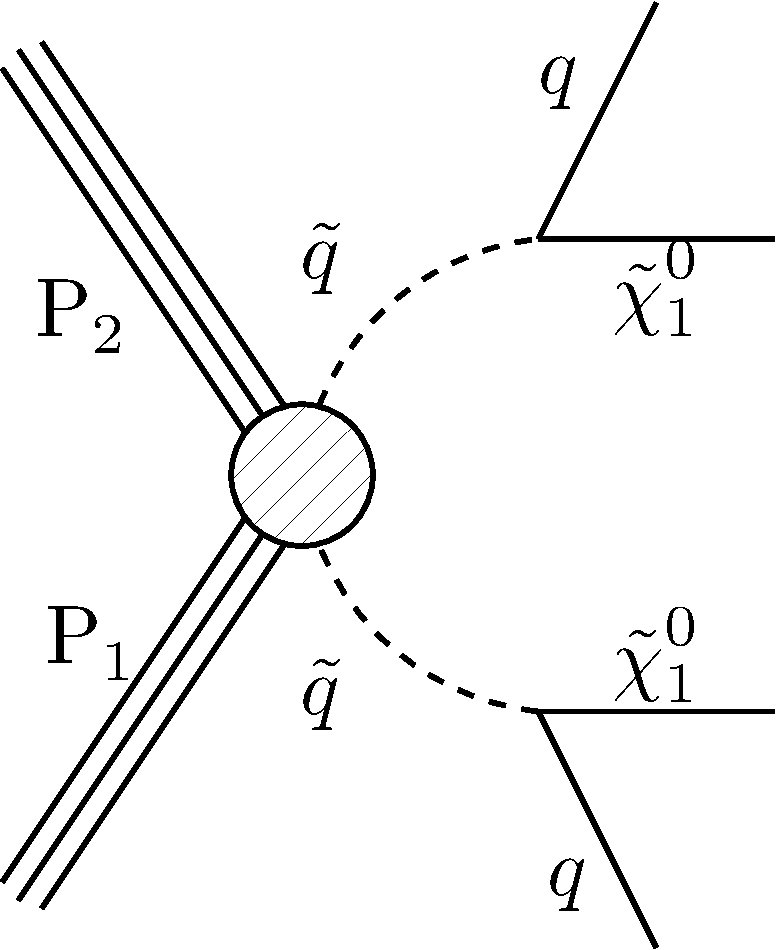
\includegraphics[height=0.15\textwidth]{figures/diagrams/alexis/feyn/T2qq_feyn}
%      \label{fig:T2qq_feyn}
%    } ~~
%    \subfigure[\texttt{T1bbbb}]{
%      
\includegraphics[height=0.15\textwidth]{figures/CMS_logo}%diagrams/misc/T1bbbb_feyn}
%      \label{fig:T1bbbb_feyn}
%    } ~~
%    \subfigure[\texttt{T1tttt}]{
%      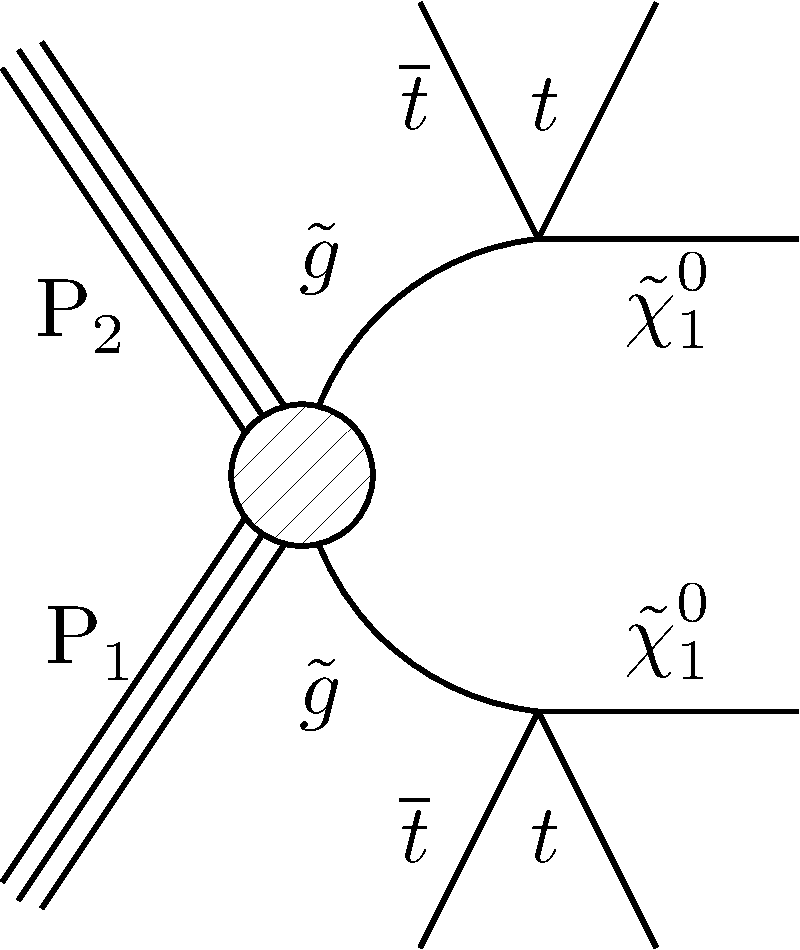
\includegraphics[height=0.15\textwidth]{figures/diagrams/alexis/feyn/T1tttt_feyn}
%      \label{fig:T1tttt_feyn}
%    } ~~
%    \subfigure[\texttt{T1ttbb}]{
%      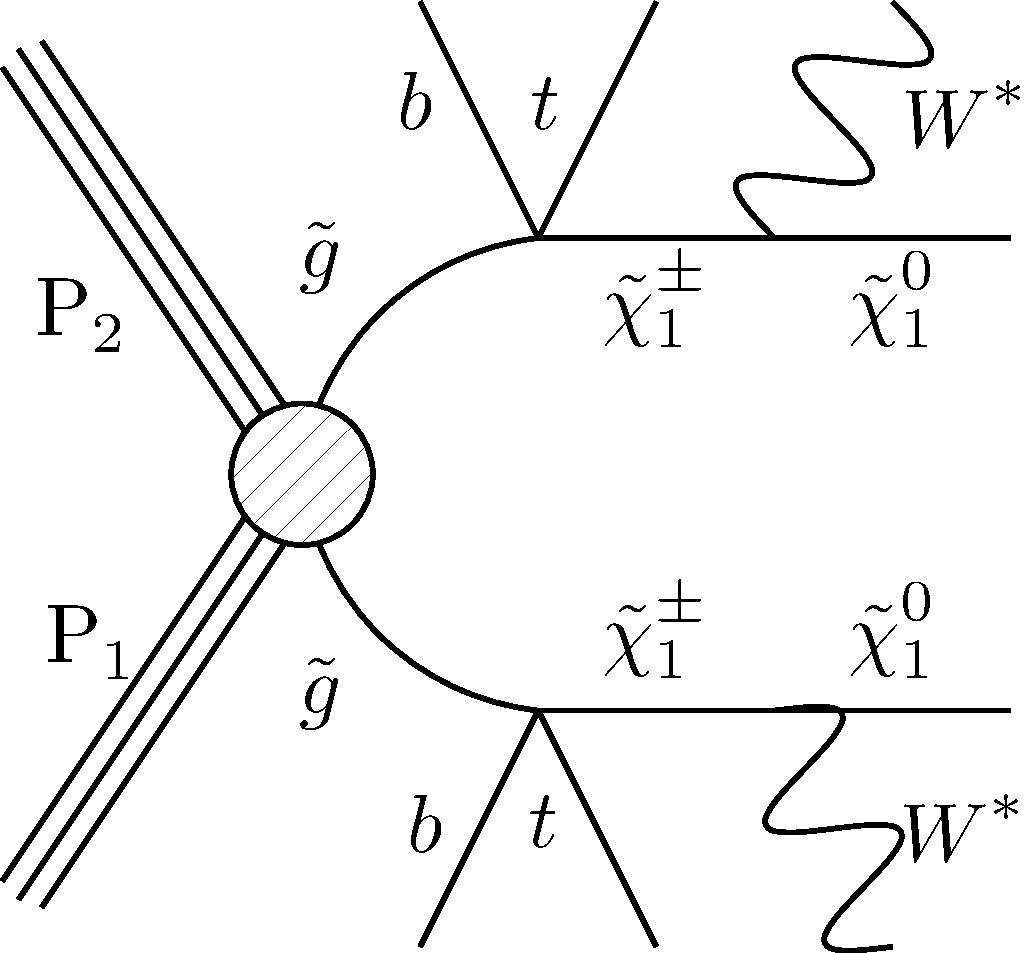
\includegraphics[height=0.15\textwidth]{figures/diagrams/alexis/feyn/T5ttbb_feyn}
%      \label{fig:T1ttbb_feyn}
%    } \\
%    \subfigure[\texttt{T5tttt}]{
%      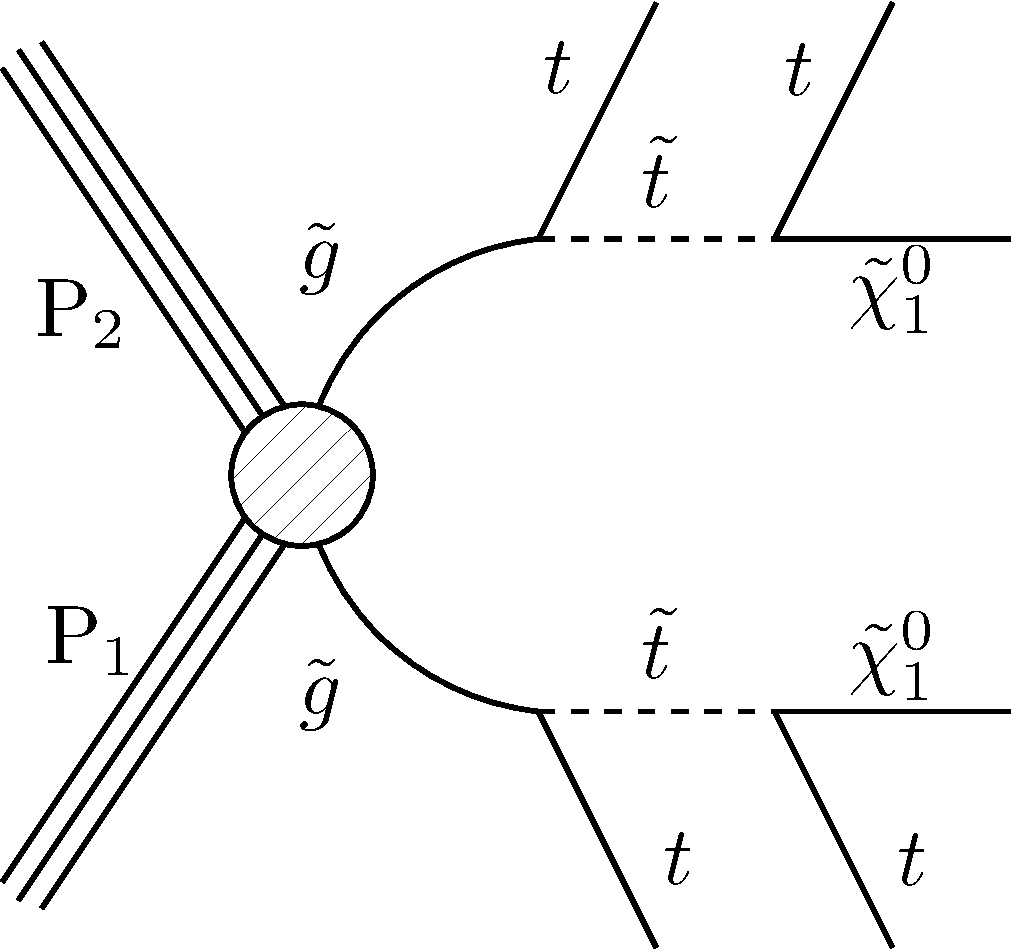
\includegraphics[height=0.15\textwidth]{figures/diagrams/alexis/feyn/T5tttt_feyn}
%      \label{fig:T5tttt_feyn}
%    } ~~
%    \subfigure[\texttt{T5ttcc}]{
%      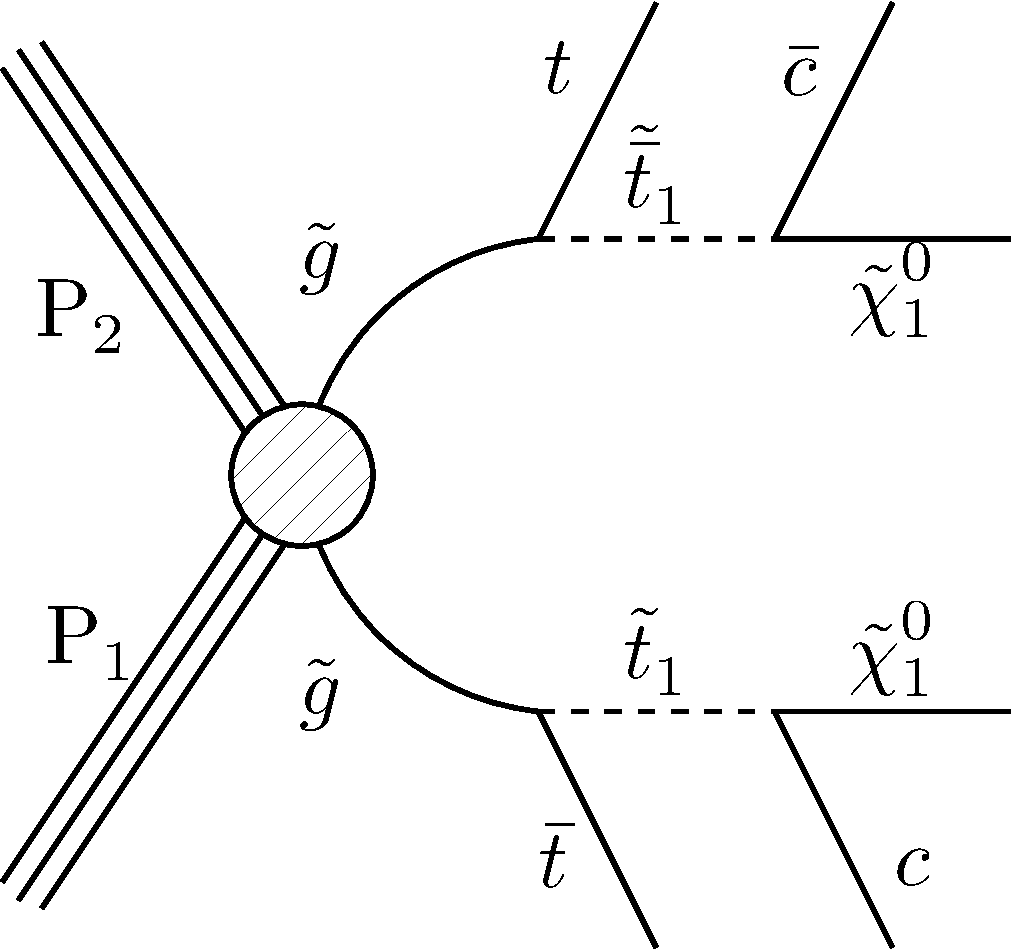
\includegraphics[height=0.15\textwidth]{figures/diagrams/misc/T5ttcc_feyn}
%      \label{fig:T5ttcc_feyn}
%    } ~~
%    \subfigure[\texttt{T5tttt\_degen}]{
%      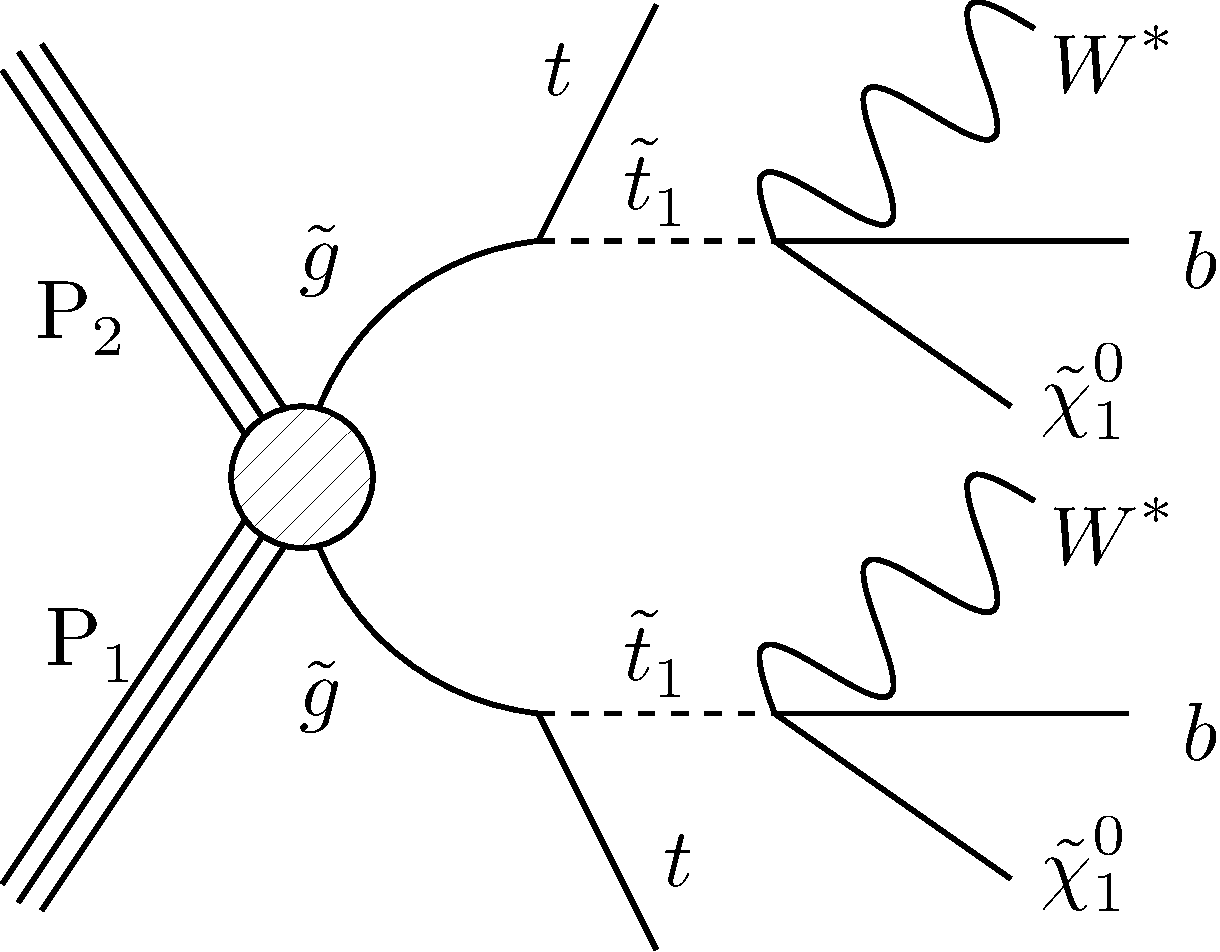
\includegraphics[height=0.15\textwidth]{figures/diagrams/misc/T5tttt_degen_feyn}
%      \label{fig:T5tttt_degen_feyn}
%    } ~~
%    \subfigure[\texttt{T2bb}]{
%      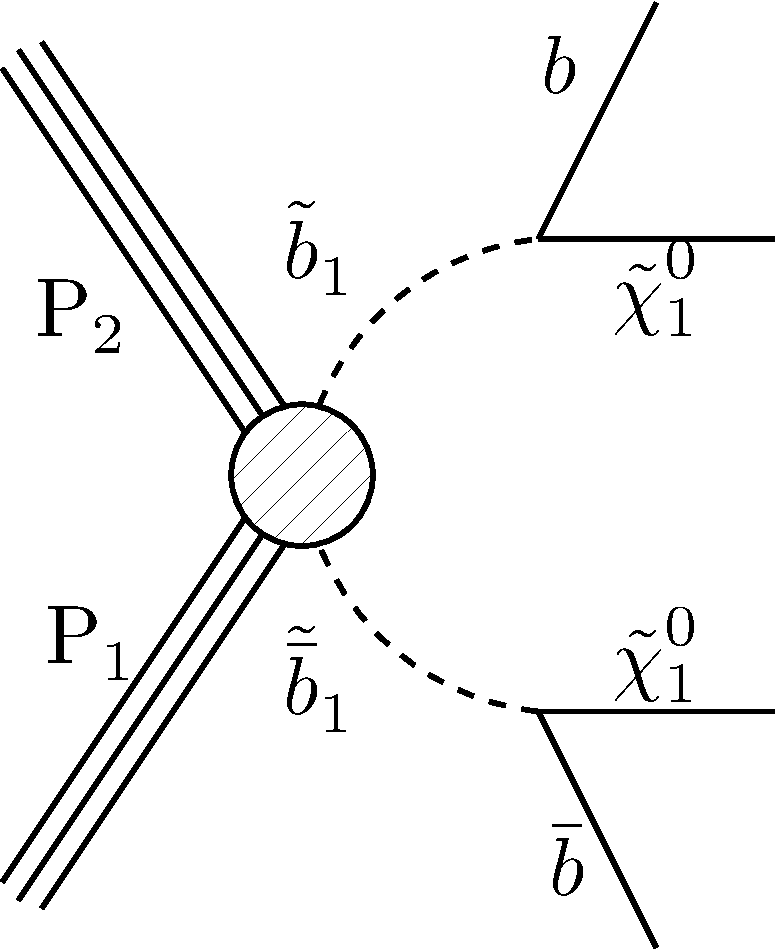
\includegraphics[height=0.15\textwidth]{figures/diagrams/alexis/feyn/T2bb_feyn}
%      \label{fig:T2bb_feyn}
%    } ~~
%    \subfigure[\texttt{T2tb}]{
%      
\includegraphics[height=0.15\textwidth]{figures/CMS_logo}%diagrams/misc/T2tb_feyn}
%      \label{fig:T2tb_feyn}
%    } \\
%    \subfigure[\texttt{T2tt}]{
%      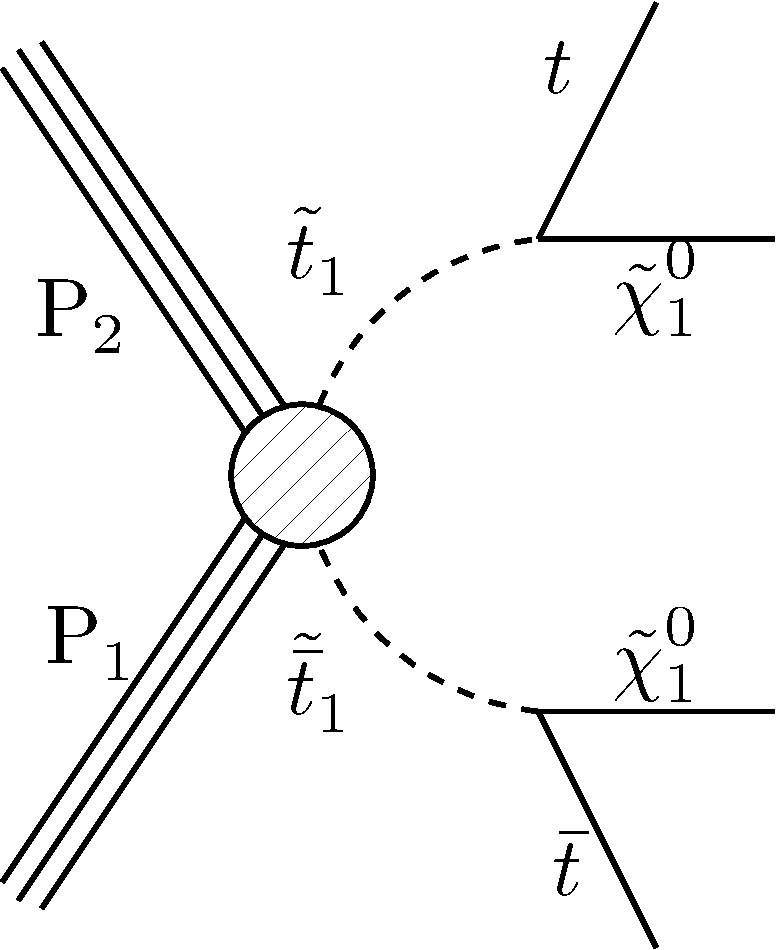
\includegraphics[height=0.15\textwidth]{figures/diagrams/alexis/feyn/T2tt_feyn}
%      \label{fig:T2tt_feyn}
%    } ~~
%    \subfigure[\texttt{T2cc}]{
%      
\includegraphics[height=0.15\textwidth]{figures/CMS_logo}%diagrams/misc/T2cc_feyn}
%      \label{fig:T2cc_feyn}
%    } ~~
%    \subfigure[\texttt{T2tt\_degen}]{
%      
\includegraphics[height=0.15\textwidth]{figures/CMS_logo}
%      \label{fig:T2tt_degen_feyn}
%    } ~~
%    \subfigure[\texttt{T2tt\_mixed}]{
%      
\includegraphics[height=0.15\textwidth]{figures/CMS_logo}
%      \label{fig:T2tt_mixed_feyn}
%    } ~~
%    \caption{ Simplified model diagrams that represent unique
%      production and decay modes of supersymmetric
%      particles. Three-body decays of gluinos are assumed to proceed
%      through off-shell squarks. Additional assumptions concerning the
%      mass relations and branching ratios are specified in
%      Table~\ref{tab:simplified-models}. The diagrams labelled
%      \texttt{T1qqqq} and \texttt{T2qq} depict, respectively, the
%      gluino-mediated and direct production of light-flavour
%      squarks. The diagrams labelled \texttt{T1bbbb}, \texttt{T1tttt},
%      and \texttt{T1ttbb} depict models involving the gluino-mediated
%      production of off-shell third-generation squarks. The diagrams
%      labelled \texttt{T5tttt}, \texttt{T5ttcc}, and
%      \texttt{T5tttt\_degen} depict ``natural'' models comprising
%      gluino-mediated production of on-shell top squarks. Finally, the
%      remaining six diagrams depict the direct production of on-shell
%      third-generation squarks, decaying via a range of channels.  }
%    \label{fig:simplified-models}
%  \end{center}
%\end{figure*}




%& PU & Trigger & XS [pb] & XS [fb] (3sf)
%& 1-5  & 1-3  & 0.0460525 & 46.1             
%& 1-9  & 5-13 & 0.677478  & 677\phantom{.0}  
%                                             
%& 1-10 & 1-6  & 0.0439731 & 44.0             
%& 1-15 & 3-12 & 1.08047   & 1080\phantom{.0} 
%                                             
%& 1-4  & 1-3  & 0.0141903 & 14.2             
%& 1-20 & 1-15 & 0.325388  & 325\phantom{.0}  
%                                             
%& 1-4  & 1-3  & 0.0460525 & 46.1             
%& 1-13 & 1-10 & 1.4891    & 1490\phantom{.0} 
%                                             
%& 1-18 & 1-4  & 0.0460525 & 46.1             
%& 1-12 & 1-14 & 0.325388  & 325\phantom{.0}  
%                                             
%& 2-6  & 3-6  & 1.4891    & 1490\phantom{.0} 
%& 4-4  & 3-10 & 3.5251    & 3530\phantom{.0} 
%                                             
%& 1-9  & 2-6  & 0.0856418 & 85.6             
%& 1-8  & 4-7  & 2.26585   & 2270\phantom{.0} 
%                                             
%& 3-5  & 3-4  & 0.163491  & 16.3             
%& 1-20 & 1-11 & 1.4891    & 1490\phantom{.0} 
%                                             
%& 1-16 & 2-12 & 0.0283338 & 28.3             
%& 1-11 & 3-3  & 2.61162   & 2610\phantom{.0} 
%                                             
%& 1-8  & 1-12 & 0.174599  & 175\phantom{.0}  
%& 1-12 & 5-7  & 3.78661   & 3790\phantom{.0} 
%                                             
%& 1-13 & 2-11 & 0.0670476 & 67.0             
%& 1-10 & 5-9  & 3.78661   & 3790\phantom{.0} 
%                                             
%& 1-26 & 5-16 & 5.60471   & 5600\phantom{.0} 
%                                             
%& 1-11 & 2-18 & 8.51615   & 8520\phantom{.0} 
%                                             
%& 1-22 & 2-16 & 8.51615   & 8520\phantom{.0} 

%\clearpage
%\begin{figure*}[thp!]
%  \begin{center}
%    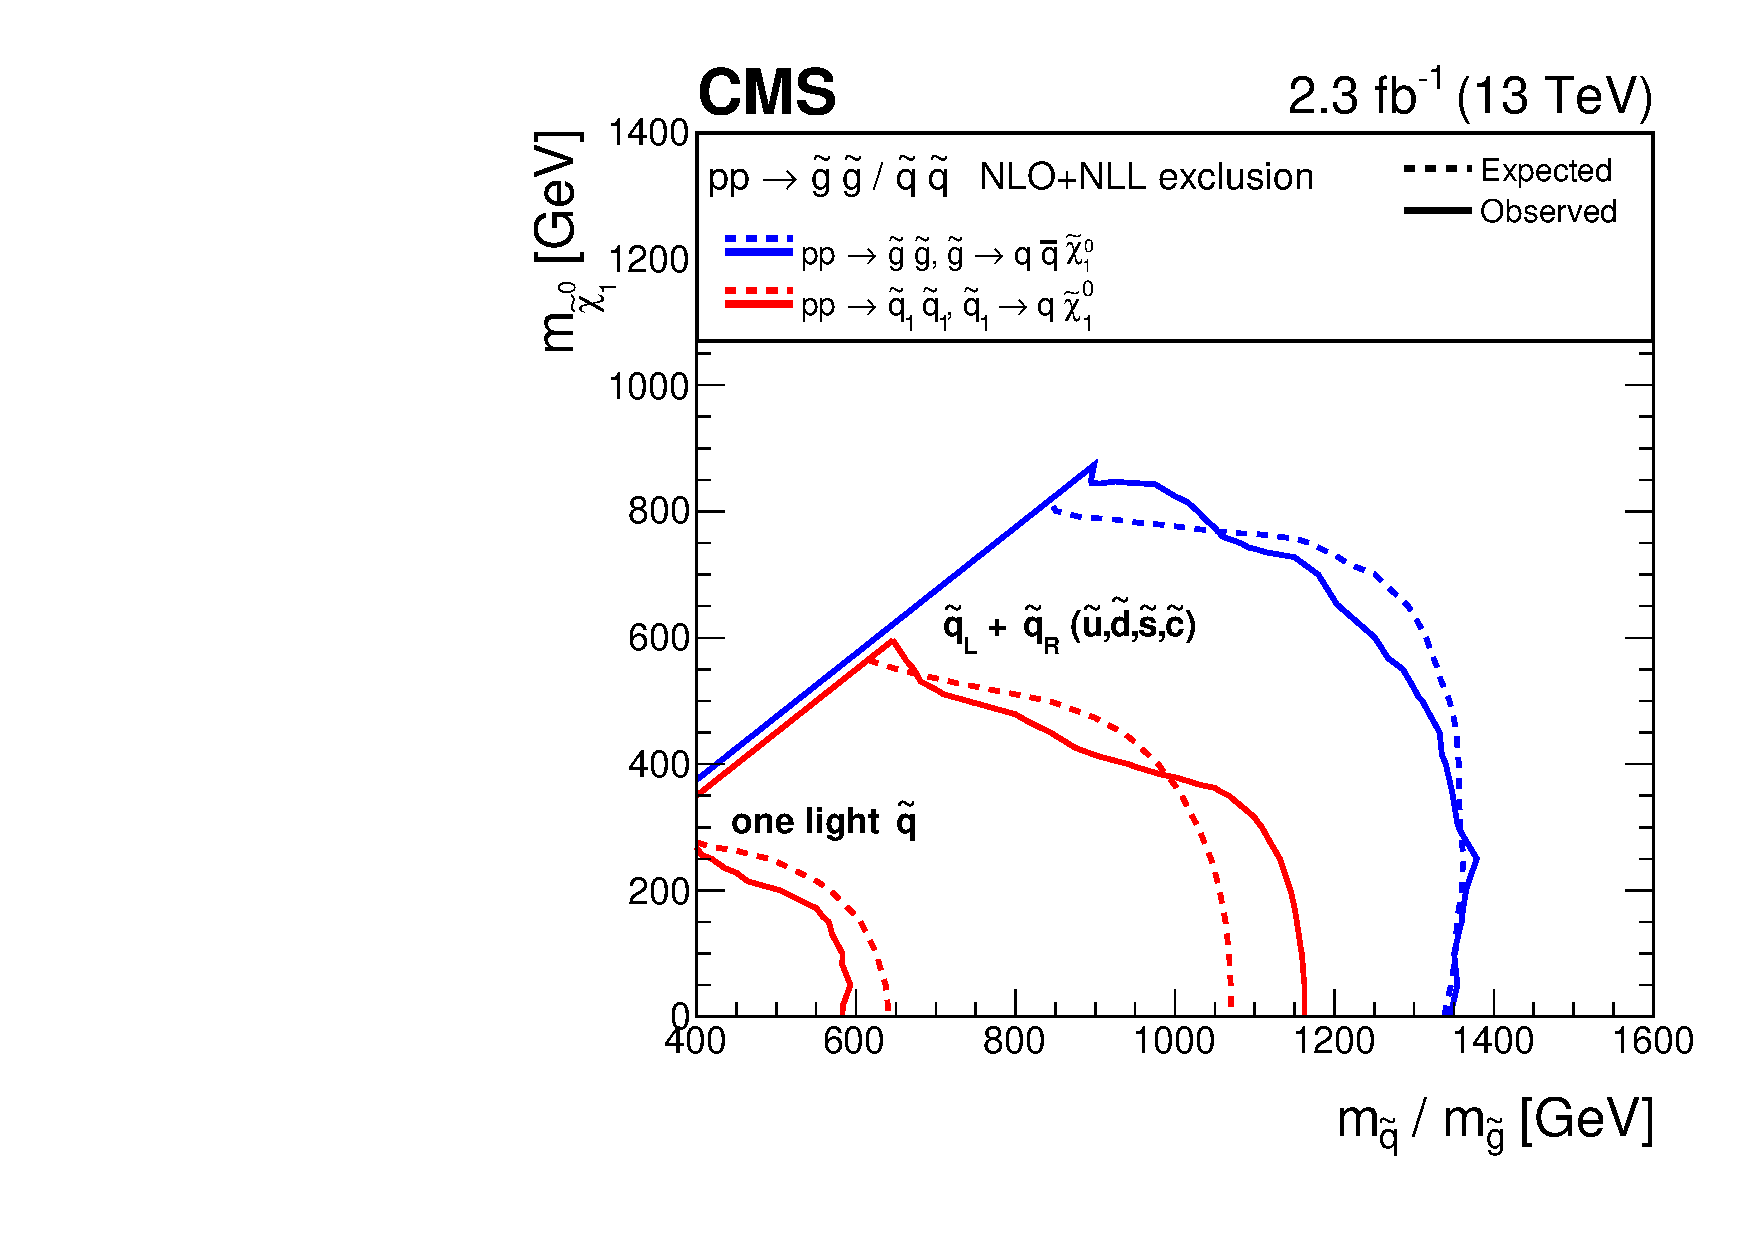
\includegraphics[width=0.49\textwidth]{figures/limits/v1/mixSUMMARY.pdf}
%    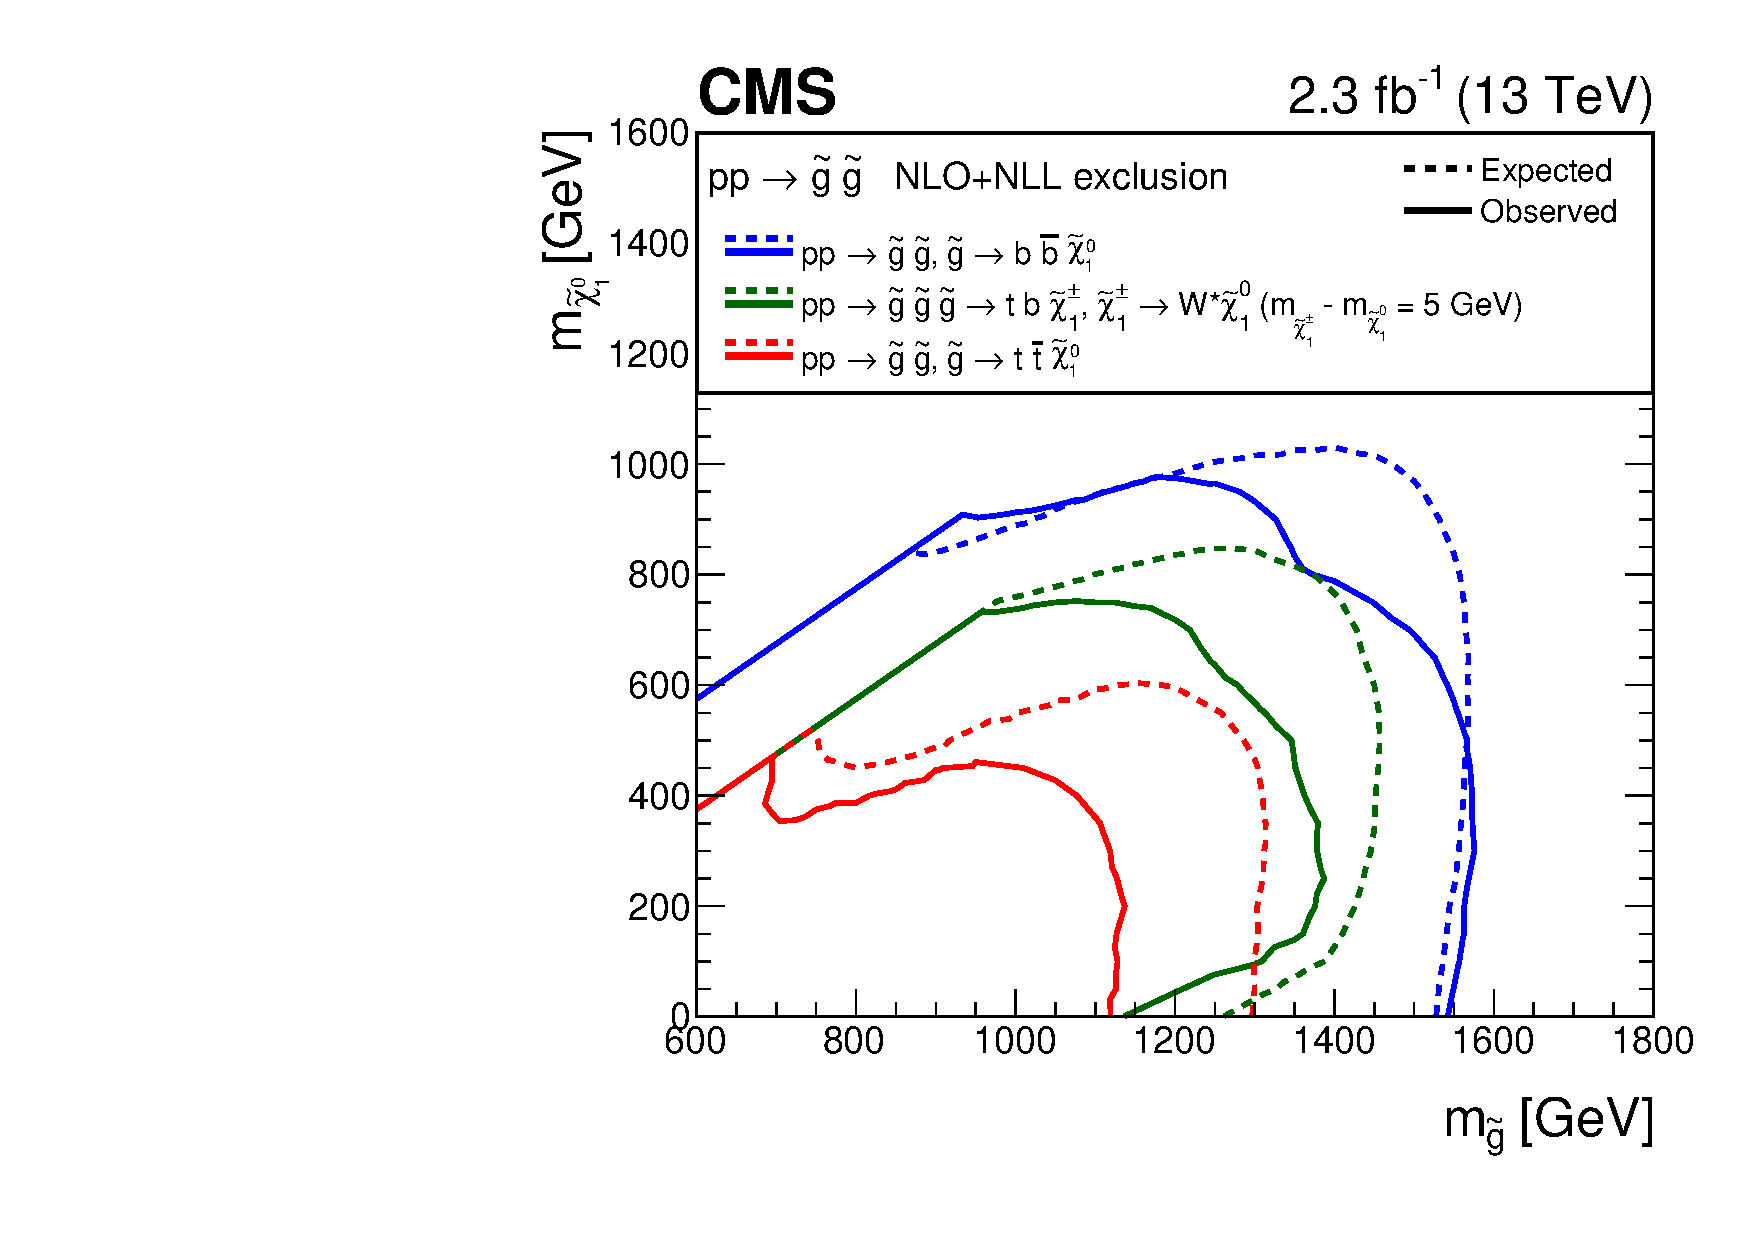
\includegraphics[width=0.49\textwidth]{figures/limits/v1/gluinoSUMMARY.pdf} \\
%    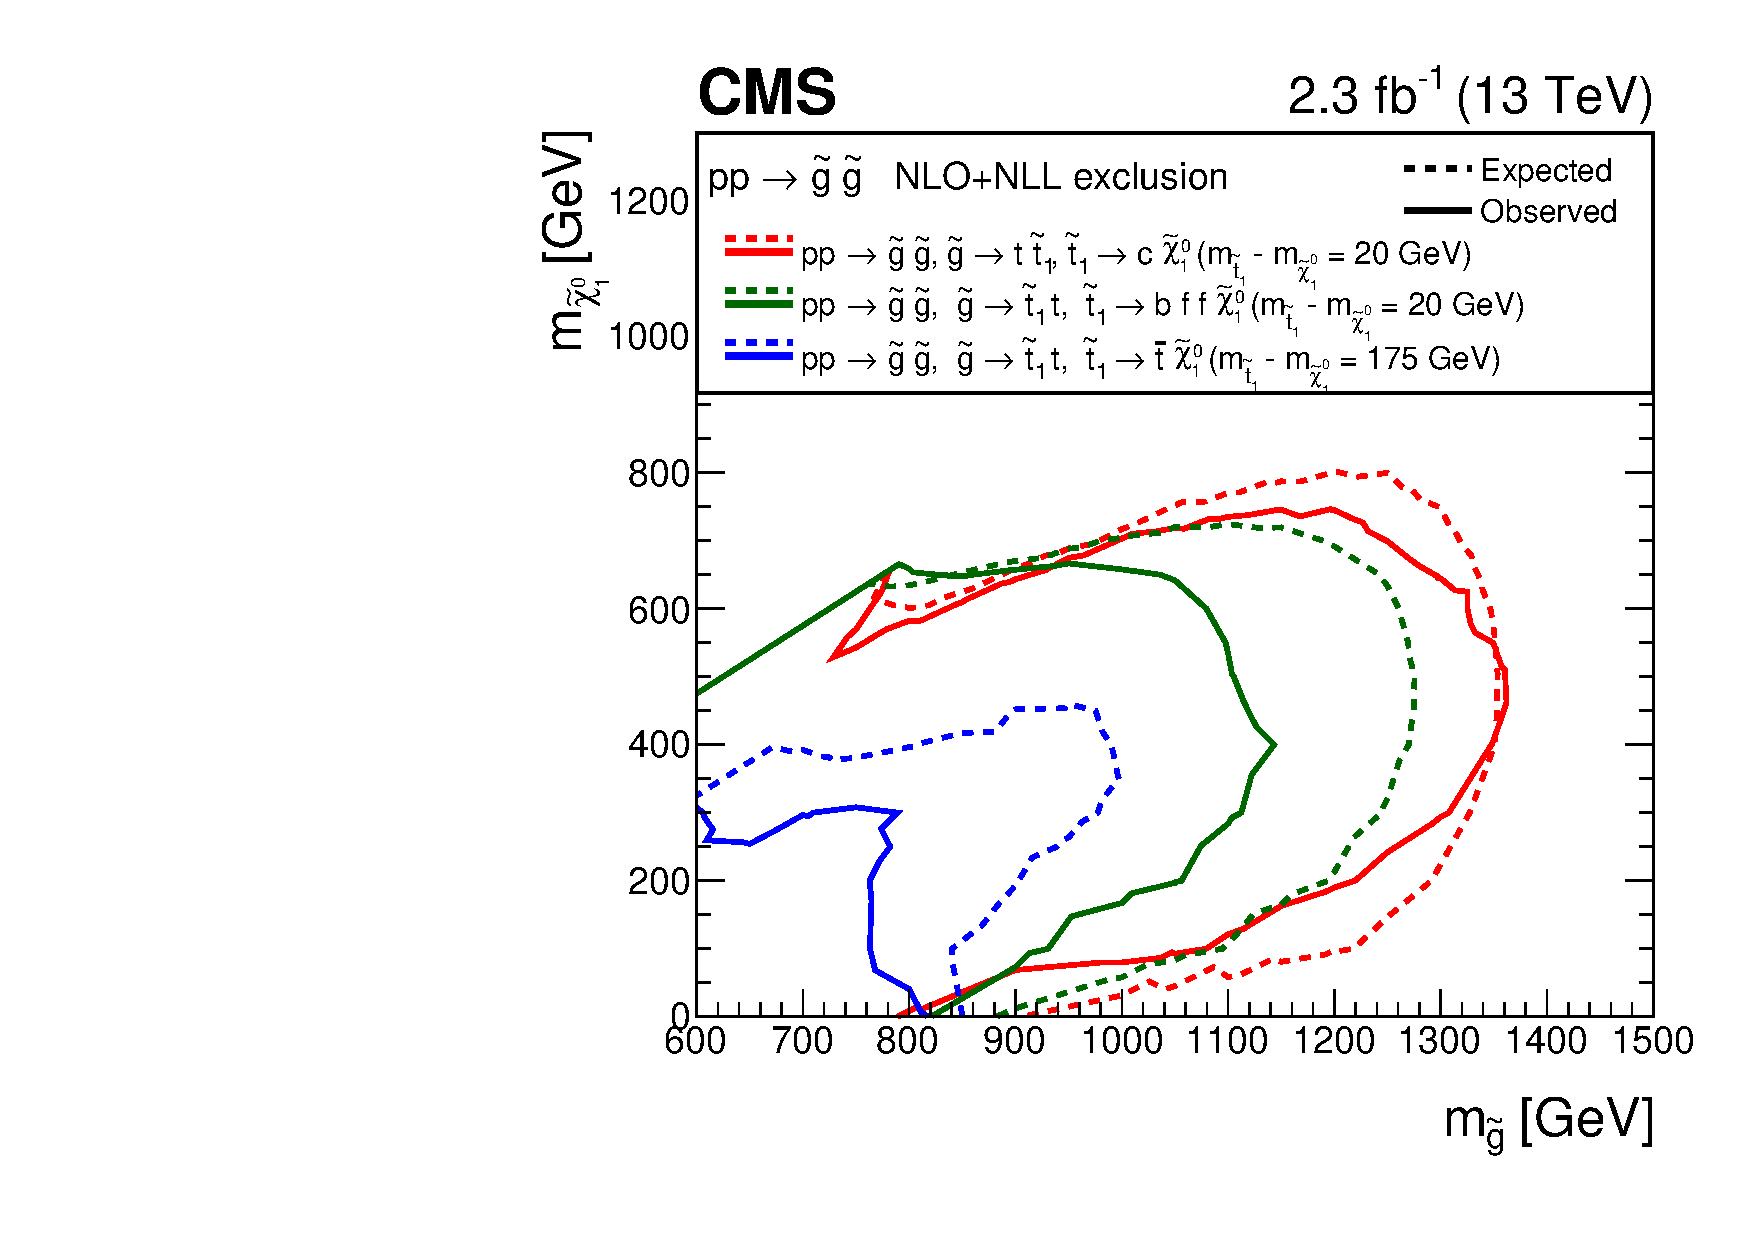
\includegraphics[width=0.49\textwidth]{figures/limits/v1/naturalSUMMARY.pdf}
%    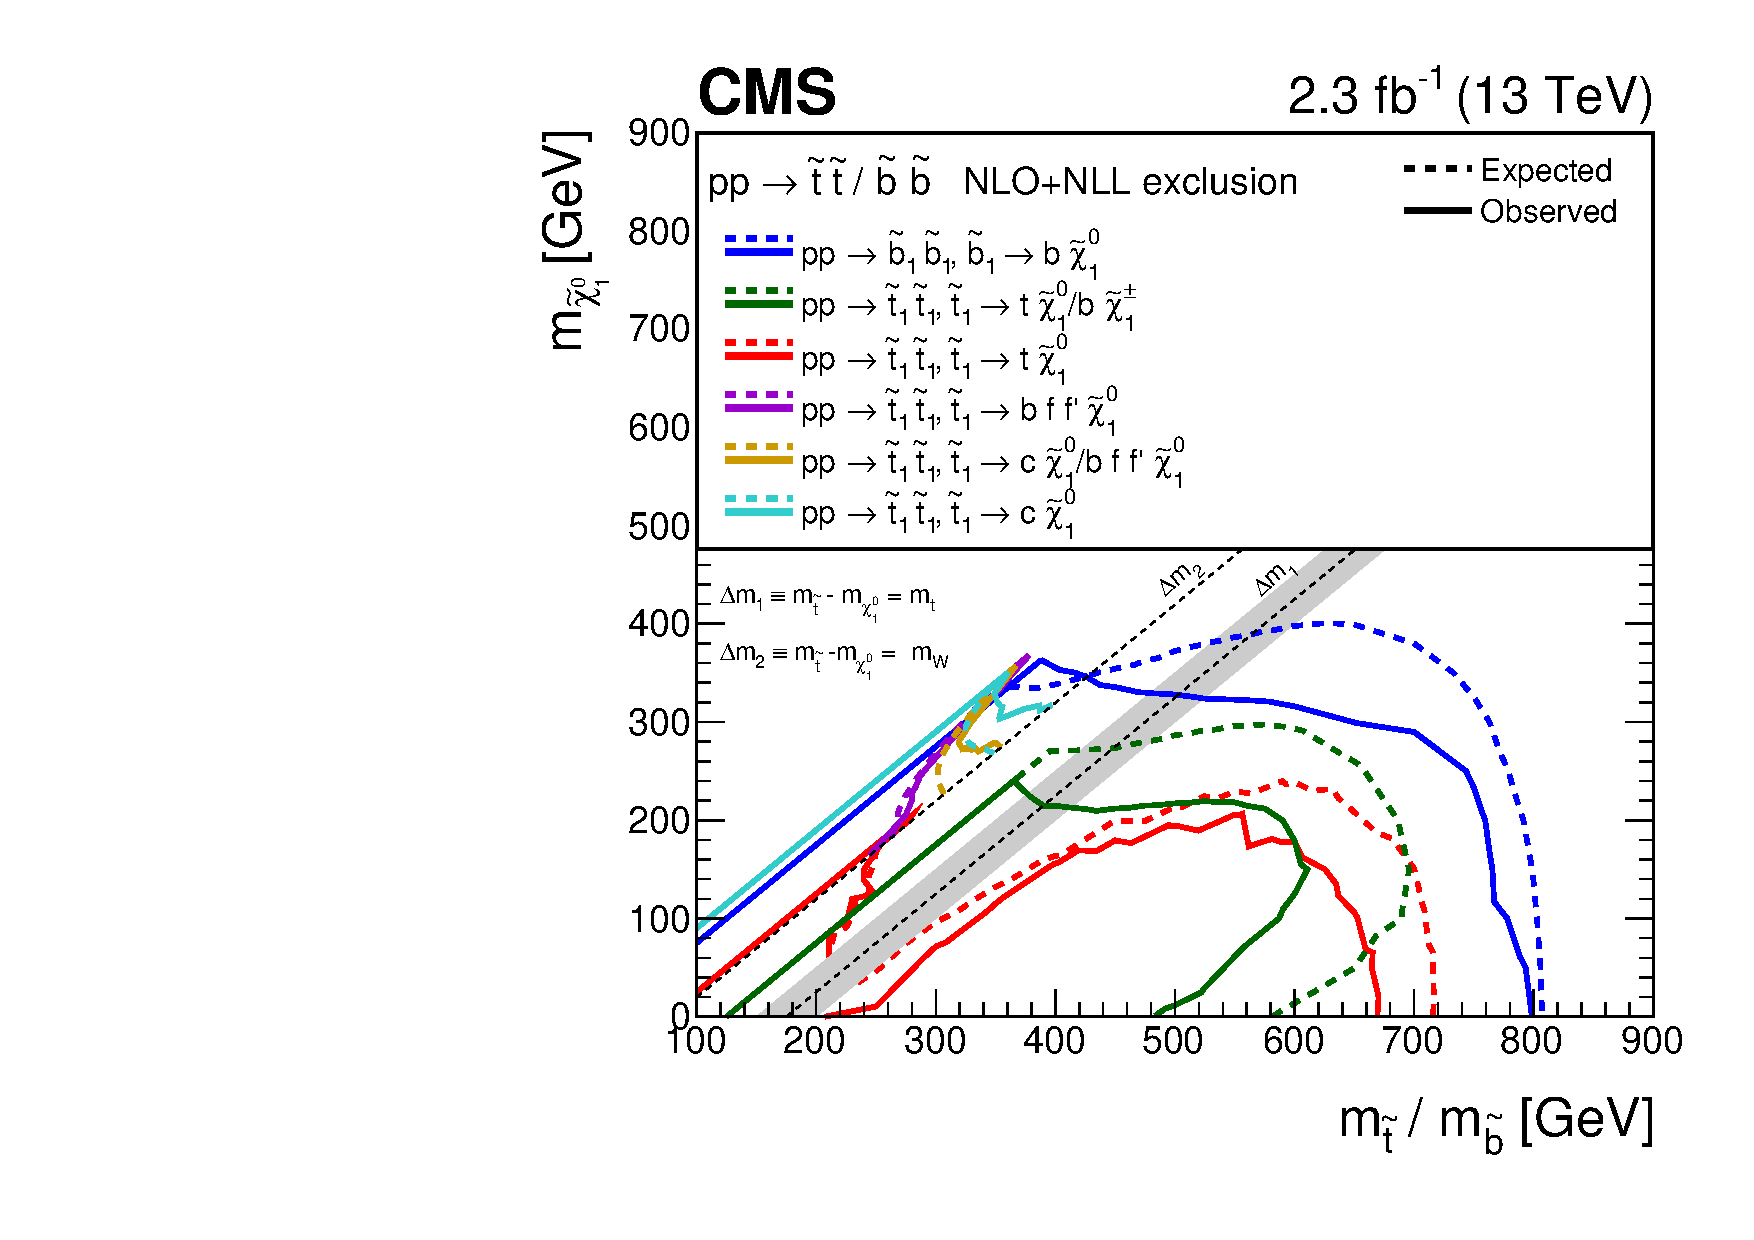
\includegraphics[width=0.49\textwidth]{figures/limits/v1/allThirdGenSUMMARY.pdf} \\
%    \caption{Observed upper limit in cross section at 95\% CL
%      (indicated by the colour scale) for simplified models that
%      assume the pair production of gluinos, as a function of the
%      gluino and $\chiz_{1}$ masses for gluino three-body decays to
%      $b\bar{b}\chiz_{1}$ (top left), $q\bar{q}\chiz_{1}$ (top right) and $t\bar{t}\chiz_{1}$ (bottom center). 
%      The black solid thick (thin) line indicates the observed mass
%      exclusion region assuming the nominal (${\pm}1 \sigma$ theory
%      uncertainty) production cross section. The red dashed thick
%      (thin) line indicates the median (${\pm}1 \sigma$ experimental
%      uncertainty) expected exclusion.
%    }
%    \label{fig:limits-sms} 
%  \end{center}
%\end{figure*}


